%********************************************************************************
%   BracU Thesis Template (Ayesha Abed Library, Brac University)*****************
%   Filled in for: InsightLens (CSE400, Fall 2026)*******************************
%  ******************************************************************************
%   Chapter file mapping (kept from the original template):**********************
%     chapters/chapter_1.tex -> Chapter 1  Introduction**************************
%     chapters/chapter_2.tex -> Chapter 2  Literature Review*********************
%     chapters/chapter_3.tex -> Chapter 3  Requirements, Impacts and Constraints*
%     chapters/chapter_5.tex -> Chapter 4  Proposed Methodology******************
%     chapters/chapter_6.tex -> Chapter 5  Result Analysis***********************
%     chapters/chapter_9.tex -> Chapter 6  Conclusion****************************
\documentclass[Times,12pt,oneside,openany,print,index]{report}
\usepackage[a4paper,width=150mm,top=25mm,bottom=25mm]{geometry}
\usepackage[english]{babel}
\usepackage[utf8]{inputenc}
\usepackage{csquotes}
\usepackage{amsmath}
\pagestyle{plain}

\usepackage{graphicx}
\graphicspath{{images/}}
\usepackage{caption}
\usepackage{array}
\usepackage{booktabs}     % better rules in tables
\usepackage{longtable}    % tables that break across pages
\usepackage{float}
\usepackage[section]{placeins}   % keep floats inside the section that introduces them
% This document is table-heavy. With the default fractions LaTeX refuses to put a large
% table on a page that also carries text, which left several pages nearly empty.
% textfraction is the least text a page carrying floats must still show, and
% floatpagefraction is how full a page of nothing but floats has to be. Left too low,
% the first lets a page end up as two figures and one stray line, and the second hands
% a whole page to a table that does not fill it. Raised until neither happened.
\renewcommand{\topfraction}{0.9}
\renewcommand{\bottomfraction}{0.8}
\renewcommand{\textfraction}{0.12}
\renewcommand{\floatpagefraction}{0.85}
\usepackage{xcolor}
\usepackage{multirow}
\setlength{\tabcolsep}{4pt}   % the results tables are wide; 6pt each side does not fit

\usepackage[nottoc]{tocbibind}
\usepackage[normalem]{ulem}

\usepackage{hyperref}
\hypersetup{
    colorlinks=true,
    linkcolor=black,
    filecolor=magenta,
    urlcolor=black,
    citecolor=black,
    % Document properties. Without these the submitted file carries an empty
    % title and author, which is what a repository and a reader's PDF viewer
    % show in place of the real ones.
    pdftitle={A Vision-Language Based Framework for Extracting and Understanding
              Classroom Content in Dual Languages},
    pdfauthor={Syed Ar Rafi, Adiba Islam Khan, Ahsan Habib},
    pdfsubject={B.Sc. in Computer Science and Engineering, Brac University},
    pdfkeywords={Banglish, code-mixed speech recognition, Whisper, LoRA,
                 vision-language models, whiteboard reconstruction, lecture notes},
}
\urlstyle{same}

\setlength{\parindent}{0em}
\setlength{\parskip}{0.45em}
% Bibliography entries carry unbreakable identifiers (arXiv:1904.00784 and the
% like). Without this TeX cannot avoid pushing them into the margin.
\setlength{\emergencystretch}{3em}

\usepackage{nomencl}
\renewcommand{\nompreamble}{The next list describes several symbols \& abbreviations that are used later within the body of the document}
\makenomenclature

\usepackage[backend=biber,style=ieee,sorting=none]{biblatex}
\addbibresource{bibliography/references.bib}

\let\cleardoublepage=\clearpage

%******************************************************************************
% Placeholder for a figure that still has to be drawn by hand\\\\\\\\\\\\\\\\\\\
% (Canva / draw.io / Figma). Usage:\\\\\\\\\\\\\\\\\\\\\\\\\\\\\\\\\\\\\\\\\\\\\\
%   \figplaceholder{file_stem}{Caption text.}{What the drawing must show.}{7cm}\\\
% To finish it, replace the whole command with:\\\\\\\\\\\\\\\\\\\\\\\\\\\\\\\\\\\\
%   \begin{figure}[H]\centering\\\\\\\\\\\\\\\\\\\\\\\\\\\\\\\\\\\\\\\\\\\\\\\\\\\\\
%     \includegraphics[width=0.9\textwidth]{file_stem}\\\\\\\\\\\\\\\\\\\\\\\\\\\\\\\
%     \caption{Caption text.}\label{fig:file_stem}\\\\\\\\\\\\\\\\\\\\\\\\\\\\\\\\\\\\
%   \end{figure} \\\\\\\\\\\\\\\\\\\\\\\\\\\\\\\\\\\\\\\\\\\\\\\\\\\\\\\\\\\\\\\\\\\\\\
%***************************************************************************************
\newcommand{\figplaceholder}[4]{%
  \begin{figure}[H]
  \centering
  \setlength{\fboxsep}{10pt}%
  \fcolorbox{black!40}{black!5}{%
    \parbox[c][#4][c]{0.86\textwidth}{%
      \centering\small
      \textbf{[ FIGURE TO BE DRAWN: \texttt{images/#1} ]}\\[8pt]
      \itshape #3\par\vspace{8pt}
      \upshape\scriptsize
      Replace this box with\\
      \texttt{\textbackslash includegraphics[width=0.9\textbackslash textwidth]\{#1\}}%
    }%
  }
  \caption{#2}
  \label{fig:#1}
  \end{figure}%
}

\begin{document}

\thispagestyle{empty}
% ============================================================================
% TITLE PAGE
%
% Title as set by the author, 2026-09-24. If it changes, change it here and in
% core/approval.tex, which repeats it.
% ============================================================================

\begin{titlepage}
\renewcommand*{\thepage}{Title}

    \begin{center}
        \vspace*{3cm}

        {\fontsize{16pt}{22pt}\selectfont{A Vision-Language Based Framework for
        Extracting and Understanding Classroom Content in Dual Languages}
        }

        \vspace{1.5cm}

        \text{by}

        \vspace{0.5cm}

            Syed Ar Rafi\\
            {24141215}\\
            Adiba Islam Khan\\
            {24141216}\\
            Ahsan Habib\\
            {22201027}

        \vspace{1.5cm}

            A thesis submitted to the Department of Computer Science and Engineering\\
            in partial fulfillment of the requirements for the degree of\\
            B.Sc. in Computer Science and Engineering

        \vspace{2.5cm}

            Department of Computer Science and Engineering\\
            Brac University\\
            September 2026.

        \vspace{3cm}

            \copyright\ 2026. Brac University\\
            All rights reserved.

    \end{center}

\end{titlepage}

\cleardoublepage

\pagenumbering{roman}

\phantomsection
\addcontentsline{toc}{chapter}{Declaration}
% Grouped signature lines for the authors. The optional argument is the box width.
% \sigskip is the blank left above each rule for the handwritten signature. The
% approval page sets it smaller, because it carries four committee signatures and
% at this value the fourth one is pushed onto a page of its own.
\newlength\sigskip
\setlength\sigskip{1.6cm}

% Signatures. scripts/trim_signatures.py crops each scan to the writing itself
% and computes one height per file, which this reads. The heights differ because
% the signatures are different shapes: a common height would print the squarer
% ones a third narrower than the wide ones. The script equalises the size a
% reader actually judges by instead. Nothing here is typed by hand; rerun the
% script after changing a scan.
% Generated by scripts/trim_signatures.py. Do not edit by hand.
% One height per cropped signature, set so that sqrt(width*height)
% is the same for all of them and no signature exceeds 1.35cm.
\expandafter\def\csname esignh@adiba\endcsname{0.986cm}
\expandafter\def\csname esignh@ahsan\endcsname{1.048cm}
\expandafter\def\csname esignh@co-supervisor-sign\endcsname{0.939cm}
\expandafter\def\csname esignh@rafi\endcsname{1.309cm}
\expandafter\def\csname esignh@supervisor-sign\endcsname{1.119cm}


% Drops a signature into the blank gap that already sits above a rule.
% \makebox[0pt] and a \raisebox with zero height and zero depth give it no width
% and no height at all, so the rule still spans the full measure and the block
% keeps exactly the size it had unsigned. Nothing on the page moves.
\newcommand*\esignhere[1]{%
  \makebox[0pt][l]{\makebox[\linewidth][c]{%
    \raisebox{2pt}[0pt][0pt]{%
      \includegraphics[height=\csname esignh@#1\endcsname]{esign/trimmed/#1.png}}}}}

% #2 is the signature overlay, empty for an unsigned line.
\newcommand*\wildcard[3][6cm]{%
  \vspace{\sigskip}\parbox[t]{#1}{\setlength{\parskip}{0pt}#2\hrulefill\par#3}}

\section*{Declaration}

It is hereby declared that

\begin{enumerate}
  \item The thesis submitted is my/our own original work while completing my/our degree at Brac University.
  \item The thesis does not contain material previously published or written by a third party, except where this is appropriately cited through full and accurate referencing.
  \item The thesis does not contain material which has been accepted, or submitted, for any other degree or diploma at a university or other institution.
  \item We have acknowledged all main sources of help.
\end{enumerate}

\vspace{1cm}
\textbf{Student's Full Name \& Signature:}

% The university's grid, two signatures to a row. With three authors the third sits
% alone and centred on the second row, which the center environment does by itself.
% \idgap puts the id a clear space under the name instead of on the next line: the
% template does that with a ~\ spacer, which has no effect here because \wildcard
% zeroes \parskip inside the box, so the space is set explicitly.
\newcommand*\idgap{\vspace{0.38cm}}
\begingroup

    \begin{center}
        % The trailing %% matter: without them the line breaks in this source become
        % interword spaces, the row measures over the 15cm text width and the second
        % signature wraps onto a line of its own underneath the first.
        \wildcard[6.2cm]{\esignhere{rafi}}%
          {\centerline{Syed Ar Rafi}\idgap\centerline{24141215}}%
        \hspace{2.2cm}%
        \wildcard[6.2cm]{\esignhere{adiba}}%
          {\centerline{Adiba Islam Khan}\idgap\centerline{24141216}}

        \wildcard[6.2cm]{\esignhere{ahsan}}%
          {\centerline{Ahsan Habib}\idgap\centerline{22201027}}
    \end{center}

\endgroup

\pagebreak


\phantomsection
\addcontentsline{toc}{chapter}{Approval}
\section*{Approval}

The thesis titled ``InsightLens: A Vision-Language Framework for Generating Lecture Notes from Code-Mixed Banglish Classroom Videos'' submitted by
\begin{enumerate}
  \item Syed Ar Rafi ([Student ID])
  \item Adiba Islam Khan ([Student ID])
  \item Ahsan Habib ([Student ID])
\end{enumerate}

of Fall, 2026 has been accepted as satisfactory in partial fulfillment of the requirement for the degree of B.Sc. in Computer Science and Engineering in Fall 2026.

\vspace{0.5cm}
\textbf{Examining Committee:}

\vspace{1cm}

Supervisor:\
(Member)
\begin{center}
    \hspace{7cm} \wildcard{\centerline{Dr. Md. Golam Rabiul Alam} ~\ \centerline{Professor}~\ \centerline{Department of Computer Science and Engineering}~\ \centerline{Brac University} } \hspace{1cm}
\end{center}

Co-Supervisor:\
(Member)
\begin{center}
    \hspace{7cm} \wildcard{\centerline{Md. Tanzim Reza} ~\ \centerline{Lecturer}~\ \centerline{Department of Computer Science and Engineering}~\ \centerline{Brac University} } \hspace{1cm}
\end{center}

Thesis Coordinator:\
(Member)
\begin{center}
    \hspace{7cm} \wildcard{\centerline{Name of Thesis Coordinator} ~\ \centerline{Designation}~\ \centerline{Department of Computer Science and Engineering}~\ \centerline{Brac University} } \hspace{1cm}
\end{center}

Head of Department:\
(Chair)
\begin{center}
    \hspace{7cm} \wildcard{\centerline{Name of Head of Department} ~\ \centerline{Designation}~\ \centerline{Department of Computer Science and Engineering }~\ \centerline{Brac University} } \hspace{1cm}
\end{center}

\pagebreak


\phantomsection
\addcontentsline{toc}{chapter}{Ethics Statement}
\section*{Ethics Statement}

The lecture recordings used in this research are recordings of the authors themselves.
Three people appear as lecturers across the corpus, and all three are the members of
this team. Nobody outside the team was recorded, asked to teach, or asked to take part,
so the dataset contains no third-party participant and no consent was sought from anyone
other than ourselves. The recordings were made in classrooms of Brac University and in
other classrooms available to us.

No student was present as a subject of the recording. The camera faces the whiteboard
and the person writing on it, and no other person's face, name or voice forms part of
the dataset used for training or testing. No personal information about any student was
collected at any point.

The recordings, the transcripts and the reconstructed whiteboard images are kept in a
private repository and are not published. The board images show the lecturer only as an
occluding region that the pipeline removes, and the figures printed in this report were
checked so that no person other than an author is identifiable in them. No lecture
content is sent to an external service, because every model runs on our own machines.

Every transcript used as ground truth was produced and checked by members of the team,
word by word against the audio. No number in this report was written down before the
command that produces it was run, and the command for every number is recorded with the
project so that any result can be reproduced. Results that did not support our
expectations are reported in the same detail as the ones that did.


\pagebreak


\phantomsection
\addcontentsline{toc}{chapter}{Abstract}
\section*{Abstract}

University teaching in Bangladesh is usually delivered in a mixture of Bengali and
English, and students write that mixture in the Roman alphabet, a form commonly
called Banglish. Existing speech recognition does not serve it. Given a recording of
such a lecture, a multilingual model produces an English translation of what was
said, and a Bengali model writes the Bengali script that no student in the class
uses. The whiteboard, which carries most of the worked examples in a class taught
without slides, is lost entirely.

This thesis presents InsightLens, a system that takes a recorded Banglish whiteboard
lecture and produces a lecture note containing both the speech and the board. It
works in four stages. A Whisper large-v3-turbo model adapted with Low-Rank Adaptation
writes a timestamped transcript in romanized Banglish. Each whiteboard is
reconstructed from the video by tiling the frame and taking every tile from a moment
when the lecturer was not in front of it, so that every pixel of the result is
unmodified camera output. Numbered coloured boxes are drawn around each block of
writing and a vision-language model names and transcribes each box. A language model
then writes one section of notes per board, pointing the reader at the boxes, with
every quotation checked word for word against the transcript.

A corpus of 44 lecture recordings from three lecturers was collected, of which 28
lectures covering 5.15 hours were transcribed by hand against a written transcription
standard. On six whole lectures held out at random, fine-tuning cuts the median
per-clip character error rate from 67.7 to 15.8 and 16.0 per cent in two random seeds
and the word error rate from 93.9 to 42.5 and 41.7 per cent, better on 164 and 167 of
177 clips. Holding out an entire lecturer, the harder design, gives 72.8 to 50.3 per
cent character error in all six runs. Against hand-verified answer keys covering 45
boards and 436 items, changing the board-reading prompt from keywords to full
transcription raises recall from 31.2 to 88.8 per cent, while changing the model from
3 to 7 billion parameters is worth 5.3 points, so the prompt matters far more than the
model size. The generated notes carry 89.1 per cent of the board content against 37.2
per cent for a conventional summarisation prompt.

Results that did not support the design are reported in the same detail. Dual
recogniser fusion, biasing the decoder towards board words and using occlusion as a
pointer all failed. One training seed at the pre-registered learning rate diverged
completely. Measures assembled out of English strings were found, twice and
independently, to reward a model that translates code-mixed speech and to penalise one
that transcribes it, which is offered as a methodological finding for anyone
evaluating systems of this kind. The notes have not been evaluated with readers, and
that is the first item of future work.

\vspace{1cm}
\textbf{Keywords:} Code-mixed speech recognition; Banglish; Bengali-English;
Low-Rank Adaptation; Whisper; vision-language models; whiteboard reconstruction;
lecture note generation; Set-of-Mark prompting; low-resource speech
\pagebreak


\phantomsection
\addcontentsline{toc}{chapter}{Acknowledgement}
\section*{Acknowledgement}

We thank our supervisor, Dr. Md. Golam Rabiul Alam, and our co-supervisor,
Md. Tanzim Reza, for their guidance throughout this work and for the time they
gave to reviewing our results.

We thank the three lecturers who allowed their classes to be recorded. Without
those recordings there would have been no dataset, and without a dataset there
would have been no thesis.

We also thank the Department of Computer Science and Engineering of Brac
University for the support provided during the project.

\pagebreak


\renewcommand{\contentsname}{Table of Contents}
\cleardoublepage
\phantomsection
\addcontentsline{toc}{chapter}{Table of Contents}
% The document sets \parskip to 0.45em for readable body text, but the contents
% lists inherit it and gain that much between every entry. Over 91 + 19 + 23
% entries that is several pages of padding, and it left the last table entry
% stranded alone on a page of its own. Standard LaTeX sets no skip between these
% entries; the group below restores that for the three lists only.
\begingroup
\setlength{\parskip}{0pt}
\tableofcontents

\listoffigures
\listoftables
\endgroup

\printnomenclature
\addcontentsline{toc}{chapter}{Nomenclature}
\cleardoublepage

\pagenumbering{arabic}

\chapter{Introduction}
% ============================================================================
% CHAPTER 1 - INTRODUCTION
% Rubric mapping: CO1 (5 marks) is assessed from 1.1, 1.2, 1.3, 1.4, 1.5, 1.6.
% ============================================================================

\nomenclature{ASR}{Automatic Speech Recognition}
\nomenclature{WER}{Word Error Rate}
\nomenclature{CER}{Character Error Rate}
\nomenclature{LoRA}{Low-Rank Adaptation}
\nomenclature{LLM}{Large Language Model}
\nomenclature{VLM}{Vision-Language Model}
\nomenclature{SoM}{Set-of-Mark prompting}
\nomenclature{LOSO}{Leave-One-Speaker-Out}
\nomenclature{Banglish}{Bengali-English code-mixed speech written in the Roman alphabet}
\nomenclature{GPU}{Graphics Processing Unit}
\nomenclature{OCR}{Optical Character Recognition}

\section{Background}

Teaching in Bangladeshi universities rarely happens in a single language. In a
typical computer science class the lecturer explains an idea in Bangla, names it
in English, writes the English term on the whiteboard, and then returns to Bangla
for the worked example. A single sentence can carry both languages, as in
\textit{``erpor e ami ki korbo? not korbo''}, where the grammar is Bengali and the
technical word is English. When students write this mixture down they almost never
use the Bengali script. They type it in Roman letters, and the result is commonly
called Banglish. Students take notes in Banglish, message each other in Banglish
and search in Banglish, so Banglish is the written form that matches how the class
actually sounds.

Automatic speech recognition has become very good at the languages it was built
for. Large multilingual models such as Whisper are trained on hundreds of
thousands of hours of audio and reach usable accuracy on many languages, including
Bengali \cite{radford2023whisper}. These models, however, assume that an utterance
belongs to one language. Whisper is given a language token and a task token, and
for Bengali audio that contains English words it usually produces a fluent English
translation rather than a transcript of what was said. A Bengali speech model of
the other kind, trained only on clean Bengali, writes everything in Bengali script
and turns the English technical terms into Bengali spellings. Neither output is
the lecturer's own words, and neither can be searched by a student who writes in
Banglish.

Speech is also only half of a whiteboard lecture. In the classrooms recorded for
this work the lecturer does not use slides. Definitions, truth tables, SQL
queries, IP address calculations and diagrams appear on the board and are then
talked about. A note taken from the audio alone loses all of it. Reading the board
from the video is not a simple screenshot problem either, because the lecturer
stands in front of what he has just written, the room lights leave glare on the
surface, and the board is wiped and reused several times in one class.

Three developments make a system that handles both sides practical on ordinary
hardware. Parameter efficient fine-tuning, in particular Low-Rank Adaptation
\cite{hu2022lora}, allows a large speech model to be adapted on a few hours of new
speech by training a small number of extra weights, which fits in the memory of a
single desktop graphics card. Open vision-language models such as Qwen2.5-VL read
text inside an image and answer questions about it without any dedicated OCR stage
\cite{bai2025qwen25vl}. Instruction tuned language models such as Qwen2.5-7B can
take the transcript and the board content together and write a structured
document from them \cite{qwen2025qwen25}.

This thesis brings the three together into one system, called InsightLens. A
lecture video goes in. What comes out is a lecture note that a student can read,
containing the board redrawn without the lecturer in front of it, numbered
coloured boxes around each part of the board, an explanation written from the
lecturer's own words, and quotations of the lecturer that have been checked
against the transcript. The note is produced in two versions, one in Banglish and
one in English, so that both an English-medium reader and a student who is more
comfortable in the mixed language can use it.

\figplaceholder{fig-1-1-overview}{The InsightLens idea in one picture. A recorded
Banglish lecture is turned into a readable lecture note that contains both the
speech and the whiteboard.}{A simple left to right drawing. On the left, a camera
icon and the words ``Banglish lecture video''. In the middle, three boxes stacked
or in a row: ``Speech to Banglish text'', ``Whiteboard reconstructed and read'',
``Notes written''. On the right, a picture of the finished note page with a
coloured board image and numbered boxes. Keep it non-technical, this is the
opening figure.}{6.5cm}

\section{Rational of the Study or Motivation}

The direct motivation is that a student who misses a class, or who cannot follow
the English terms at the speed they are spoken, currently has nothing useful to
fall back on. A recording of the class exists, but three hours of video is not a
study aid. Running that video through any available transcription service returns
either English prose that was never spoken or Bengali script that no one in the
class writes. Neither helps the student revise, and neither contains the
whiteboard, which is where most of the examples live.

The second motivation is cost. Producing a correct Banglish transcript by hand is
slow work. In this project it took about one hour of human effort for every ten
minutes of video, because existing tools give the transcriber almost nothing
usable to start from. At that rate a single semester of one course is weeks of
work. If a model can be brought close enough to the lecturer's words that a human
only has to fix small errors, the cost of making lecture material accessible drops
sharply. That is a realistic goal, and it is measurable, which is why the error
rate of the speech model is treated in this thesis as a result in its own right
rather than as an internal detail.

The third motivation is that the research gap is specific and checkable. Code
switched speech recognition has been studied for Hindi-English and for several
other language pairs, and Bengali speech recognition has its own literature. What
is missing is the combination that a Bangladeshi classroom actually needs, which
is recognition of Bengali-English code-mixed speech written back in the Roman
alphabet, evaluated on real lectures rather than on read or synthetic speech.
Chapter 2 reviews the systems that come closest, including recent Bengali-English
code-switched models, and states exactly which part of this work is new and which
part is not.

Finally, the whiteboard side of the problem has a practical value beyond note
taking. A clean picture of every board a lecturer wrote, with the person removed
and the content read out as text, is useful on its own. It can be searched, it can
be pasted into a study guide, and it gives a student a record of a class that was
never written down anywhere else.

\section{Problem Statement}

The problem this thesis addresses is the following. Given an ordinary recording of
a university lecture delivered in Bengali-English code-mixed speech, in a room
with a whiteboard and no slides, produce a lecture note that is faithful to what
the lecturer said and to what the lecturer wrote.

This breaks into four smaller problems, each of which was confirmed by measurement
on our own recordings before any solution was attempted.

\textbf{The speech is not transcribed by existing systems.} On the six lectures
held out for testing in this work, off-the-shelf Whisper large-v3-turbo makes a
median character error rate of 67.7 per cent and a median word error rate of 93.9
per cent against human references. The failure is not random noise. The model
translates the speech into English and, on thirteen of the one hundred and
seventy-seven test clips, falls into a repetition loop and repeats the same phrase
until it hits the token limit. Table \ref{tab:motivating_example} shows one
segment of a digital logic class in three versions.

\begin{table}[H]
\centering
\caption{One segment of lecture BanglaASR7, as spoken and as produced by two
models. The reference is the human transcript. The off-the-shelf model translates
and then loops. The fine-tuned model writes what was said.}
\label{tab:motivating_example}
\begin{tabular}{p{2.6cm}p{10.5cm}}
\toprule
\textbf{Source} & \textbf{Text} \\
\midrule
Human reference &
\textit{done. so x-or jodi amra bujhe jai tahole last je exclusive gate sheitao
kintu amader bujha easier hoye jabe.} \\
\addlinespace
Off-the-shelf Whisper &
\textit{so, x or gate and x or gate and x or gate and x or gate and \dots}
(repeats until the token limit) \\
\addlinespace
Fine-tuned Whisper &
\textit{done. so, x or jodi amra bujhe jai, tahole last je exclusive gate, sheta o
kintu amader bujha easier hoye chabe.} \\
\bottomrule
\end{tabular}
\end{table}

\textbf{The board is hidden by the person who wrote on it.} The lecturer is never
absent from the frame. Measured over seventy-nine frames of one lecture, the
lecturer covers 23.5 per cent of the writing surface in the median frame and 7.0
per cent in the best one, and no single frame is under 5 per cent. There is
therefore no moment in the video at which a clean photograph of the board can
simply be taken.

\textbf{A summarising model writes from memory instead of from the lecture.} The
first version of this pipeline asked a language model for clear notes on the
lecture. The model produced confident textbook material, including a definition of
a NAND gate that the lecturer never gave and that was wrong. Measured against
hand-checked answer keys of what was actually written on the board, those notes
contained only 37.2 per cent of the board items across thirty-five boards. The
numbers written on the board, which a model cannot guess, were the worst category
at six items found out of sixty-seven.

\textbf{The obvious ways of scoring the system are misleading.} The measure
inherited from the earlier phase of this project, a term based F1 over a fixed
list of eighty-two English words, moves by 8.1 percentage points between two
training runs on identical data, and it moves in the wrong direction. A model that
transcribes the mixed speech correctly emits fewer English words than a model that
translates it, so the better transcript scores worse. Any evaluation built out of
English strings has this property, and it affects the note metric as well. Part of
the contribution of this thesis is to state this clearly and to measure around it.

\section{Objective}

The aim of this study is to build and evaluate an end to end system that turns a
recorded Banglish whiteboard lecture into a usable lecture note, and to report
honestly how well each part of it works. The specific objectives are listed
below.

\begin{enumerate}
  \item To build a hand-checked corpus of Bengali-English code-mixed classroom
        speech, transcribed in the Roman alphabet according to a written
        transcription standard, large enough to fine-tune and test a speech
        model.
  \item To adapt a large pretrained speech recognition model to this speech with
        Low-Rank Adaptation, and to measure the change in word and character
        error rate against the same model without adaptation, on lectures that
        were never used for training.
  \item To choose the training settings by a procedure that is written down before
        any result is seen, scored on a separate validation set, so that the
        reported test result is not the product of repeated tuning on the test
        data.
  \item To reconstruct each whiteboard from the video without the lecturer in
        front of it, without inventing any pixel, and to measure how much of the
        writing survives.
  \item To have a vision-language model read each reconstructed board, and to
        measure how much of the board's content it recovers against answer keys
        checked by hand.
  \item To generate a lecture note in both Banglish and English that is grounded
        in the board and the transcript, that points the reader at numbered
        regions of the board image, and that only quotes the lecturer using words
        that appear in the transcript.
  \item To evaluate each stage separately with paired statistical tests, to run
        ablations that show which design choices matter, and to report the results
        that did not work as clearly as the ones that did.
\end{enumerate}

\section{Methodology in Brief}

The system runs as four stages, and each stage writes a file that the next stage
reads, so any stage can be re-run or replaced on its own.

The first stage handles the speech. The audio is extracted from the video and
split into segments at the boundaries given by the transcription standard. A
pretrained Whisper large-v3-turbo model is adapted with LoRA adapters on the
training lectures, and the adapted model writes a timestamped Banglish transcript
for a lecture it has never seen.

The second stage handles the board. Frames are taken from the video at a fixed
interval. Points at which the board is wiped are detected, which splits the
lecture into eras, one board per era. Within an era the frame is cut into
overlapping tiles, and each tile is taken from a moment when the lecturer was not
standing in front of that particular tile. The lecturer is located by a pretrained
person segmentation network together with a shadow mask. The tiles are blended
back into one image, so every pixel of the result is unmodified camera output.

The third stage reads the board. Our own code finds the blocks of writing on the
clean board, draws a numbered coloured box around each one, and a vision-language
model is asked to name and transcribe each numbered box. This is the Set-of-Mark
style of prompting \cite{yang2023som}, where the marks are drawn on the image and
the model answers per mark.

The fourth stage writes the note. For each board, a language model is given that
board's boxes, the board text, and the part of the transcript that belongs to that
board, and is asked for one section of notes that refers to the boxes by number
and colour. A checker then deletes any quotation that does not appear word for
word in the transcript, and any reference to a box number that does not exist. The
sections are assembled into a page in Markdown and in HTML with the board image
embedded.

Evaluation is done per stage and never by eye alone. Speech is scored by per-clip
median word and character error rate against human transcripts, with paired
Wilcoxon signed-rank tests and sign tests. The board reconstruction is scored by
the fraction of tiles that found a clear view and by a human check of whether any
writing was lost. Board reading and note quality are scored by recall of items
from hand-verified answer keys of what each board contained. Chapter 4 gives the
full detail of each stage and Chapter 5 gives the results.

\section{Scopes and Challenges}

\textbf{Scope.} The dataset is forty-four lecture recordings from three lecturers
at one university, 8.33 hours of video in total, of which twenty-eight lectures
covering 5.15 hours of speech carry hand-checked transcripts. The subjects are
introductory programming, digital logic, databases and computer networking. Every
recording is of a whiteboard class with no slides, taken with a fixed camera. The
notes are produced in Banglish and in English. Notes in the Bengali script were
considered and dropped, because they would be produced by translation alone and
would add nothing that the system itself contributes. The system is built for
recorded lectures, not for live captioning.

\textbf{What this thesis does not claim.} It does not claim that the speech model
is accurate enough to be used without a human check, and Chapter 5 states the
remaining error rate plainly. It does not claim that the generated notes are good
to read, because that has not been tested with readers. The measure used for the
notes counts whether board content reached the page, which is a real and checkable
property, but it says nothing about whether the surrounding explanation is well
written or even correct. A reader study is described in Chapter 6 as the next
step.

\textbf{Challenges.} Five difficulties shaped the work.

\begin{enumerate}
  \item \textbf{No standard spelling.} Banglish has no agreed orthography, so the
        same word can be written \textit{ami}, \textit{aami} or \textit{amee}. A
        written transcription guide was produced and enforced by a validator, and
        a spelling-tolerant version of the error rate was computed to show how
        much of the error is spelling and how much is genuine.
  \item \textbf{No dataset existed.} There is no public corpus of Bengali-English
        code-mixed classroom speech in Roman script. The corpus had to be
        recorded and transcribed by hand, and this was the single largest cost in
        the project.
  \item \textbf{Limited hardware.} All training was done on one desktop with a
        12 GB graphics card and all vision-language work on a second desktop with
        a 32 GB card. This ruled out the largest vision-language models, and the
        thesis says so rather than pretending the comparison was a free choice.
  \item \textbf{Unstable training.} The configuration chosen by the tuning
        procedure diverged on one of its two random seeds and produced a model
        worse than doing nothing. This is reported in full in Chapter 5, together
        with the settings that were stable.
  \item \textbf{Metrics that mislead.} As described in the problem statement,
        measures built out of English strings reward a model that translates. Two
        separate results in this thesis are affected by it, and both are reported
        with the explanation beside them.
\end{enumerate}

\section{Team Overview}

This thesis was carried out by a team of three students of the Department of
Computer Science and Engineering, Brac University, under the supervision of
Dr. Md. Golam Rabiul Alam and the co-supervision of Md. Tanzim Reza.

% TODO (Rafi): confirm or correct the division of work in the paragraph below
% before submission. Student IDs go on the title page and the declaration page.
The work was divided into three areas. Data collection and transcription was the
largest shared task, since every transcript in the corpus was checked word by word
against the audio by a member of the team. Model training and evaluation covered
the speech recognition experiments, the tuning procedure and the statistical
testing. The vision and note generation side covered board reconstruction, the
vision-language prompting and the note builder. All three members took part in the
verification of the board answer keys, which had to be done by a person looking at
the board image without seeing any model output, and in the writing of this
report.


\chapter{Literature Review}
% ============================================================================
% CHAPTER 2 - LITERATURE REVIEW
% Rubric mapping: CO9 (5 marks) is assessed from 2.1, 2.2, 2.3.
% Works cited here were checked against their sources in September 2026. Where a
% system is a public model or repository rather than a peer-reviewed paper, the
% text says so.
% ============================================================================

\section{Preliminaries}

\subsection{Code-mixing and Banglish}

Code-switching is the use of more than one language by the same speaker in the same
conversation. Two cases are usually distinguished. Inter-sentential switching means the
speaker finishes a sentence in one language and begins the next in another.
Intra-sentential switching, also called code-mixing, means the switch occurs inside a
single sentence. The second case is harder for speech systems, because the utterance
cannot be assigned to one language and handed to one monolingual model
\cite{agro2025cssurvey}.

Bangladeshi classroom speech is strongly intra-sentential. In the recordings used here a
single clause regularly carries a Bengali verb, an English noun phrase and an English
technical term, so the speech is Bengali in grammar and often English in content words.

The written form matters as much as the spoken one. Bengali has its own script, but it is
also widely written in the Roman alphabet in informal digital text, a form usually called
Banglish. There is no spelling standard, so the same word appears as \textit{ami},
\textit{aami} or \textit{amee} depending on the writer. Romanised Bangla is now an object
of study in natural language processing in its own right. BanglaTLit, for example, is a
benchmark of 42,700 romanised Bangla samples with a pre-training corpus of 245,700 more,
built for converting romanised Bangla back into the Bengali script
\cite{fahim2024banglatlit}. Work of this kind establishes romanised Bengali as a real
written form with real users, which is the reason it was chosen here as the output of the
speech model rather than the Bengali script.

\subsection{Speech recognition, error rates and the models used}

Automatic speech recognition takes an audio signal and returns text. Its usual measure is
the word error rate, the number of word substitutions, insertions and deletions needed to
turn the output into the reference divided by the number of reference words. Character
error rate is the same calculation over characters. Both can exceed 100 per cent when the
system produces more text than was spoken.

Two properties of these measures shaped how results are reported in this research. A single
long wrong output for one short clip pushes a mean error rate above 100 per cent and
hides everything else, so medians over clips are reported and systems are compared clip
by clip. Word error rate is also unkind to a language with no spelling standard, because
two acceptable spellings of the same word count as an error; Section \ref{sec:cs-metrics} reviews what
the code-switching literature does about this.

Modern recognisers are built in one of two ways, and the difference matters later in this
research because the two write their output differently. The first is connectionist temporal
classification, which scores an alignment between audio frames and a fixed set of output
symbols \cite{graves2006ctc}. A model of this kind can only ever emit characters that are
in its output alphabet, which is decided before training. The second is the encoder-decoder
transformer \cite{vaswani2017attention}, which generates text one token at a time and can
in principle produce any string its tokeniser can represent. Conformer models add
convolution to the transformer encoder and are a common choice for speech
\cite{gulati2020conformer}.

Most recent recognisers for languages with little transcribed audio start from a model
pretrained on unlabelled speech. wav2vec 2.0 learns from masked audio with a contrastive
objective \cite{baevski2020wav2vec2}, HuBERT predicts hidden units discovered by
clustering \cite{hsu2021hubert}, and WavLM extends the idea to a wider set of speech tasks
\cite{chen2022wavlm}; a review covers the family and how the approaches relate
\cite{mohamed2022sslreview}. The same recipe has been scaled across many languages at once,
first with XLSR \cite{conneau2021xlsr} and then with XLS-R \cite{babu2022xlsr2}, which is
where most published Bengali recognisers begin. WavLM is used directly in this research, not
as a recogniser but to produce a voice embedding for each recording, which is how the
lecturer of every video was confirmed. Where labelled audio is scarce, SpecAugment masks
bands of time and frequency during training and is close to standard practice
\cite{park2019specaugment}.

Whisper is a family of encoder-decoder transformer models trained on about 680,000 hours
of weakly supervised multilingual audio \cite{radford2023whisper}. Its decoder receives
special tokens stating the language and the task, where the task is either transcribe or
translate, which explains two behaviours central to this work. Because the model is told
which single language it is hearing, mixed language audio is pushed towards one of them,
and for Bengali audio containing English words the output is usually English. Because the
decoder is autoregressive with a strong internal language model, it can enter a repetition
loop in which the same phrase is emitted until the token limit is reached. The Whisper
paper proposes a fallback rule for this, in which a hypothesis whose gzip compression
ratio exceeds a threshold is decoded again with sampling \cite{radford2023whisper}, and
WhisperX avoids the problem by segmenting audio with an external voice activity detector
instead of relying on the model's own timestamps \cite{bain2023whisperx}. Loops are
reported in this research as a counted quantity.

A vision-language model takes an image and a text instruction and returns text. Open
models such as Qwen2.5-VL read text inside an image well enough that a separate optical
character recognition stage is often unnecessary \cite{bai2025qwen25vl}. Directing such a
model at a specific part of an image is a separate problem, which Set-of-Mark prompting
solves by drawing marks such as numbered boxes onto the image and asking the model to
answer per mark \cite{yang2023som}. The board reader in this research uses the same idea,
with the boxes found by our own image processing and the numbers carried through into the
generated notes.

An instruction tuned language model such as Qwen2.5-7B-Instruct can be given a transcript
and asked for structured notes \cite{qwen2025qwen25}. The risk is known from the
summarisation literature. Models produce fluent text that the input does not support, and
a study of state of the art abstractive summarisers found that a large share of generated
summaries contain hallucinated content \cite{maynez2020faithfulness}. Faithfulness asks
whether the output follows the input given to the model; factuality asks whether it is
true of the world. A lecture note must be faithful, because a statement that is true in
general but was not part of the lecture is still the wrong note.

\subsection{Fine-tuning, validation, ablation and statistical testing}

Fine-tuning means continuing to train a pretrained model on new data so that it fits a
new domain. Training all weights of a model with hundreds of millions of parameters
requires a large amount of memory, because the optimiser keeps extra state for every
parameter, and it risks destroying what the model already knows when the new dataset is
small.

A family of methods answers this by training a small number of new parameters and leaving
the pretrained weights alone. Adapters insert small trainable layers between the frozen
ones \cite{houlsby2019adapters}, and prefix tuning learns a short sequence of vectors that
is prepended to the input instead of changing any weight \cite{li2021prefix}. Low-Rank
Adaptation is the member of that family used here. A later variant, QLoRA, quantises the
frozen model to four bits so that a much larger model fits on one card
\cite{dettmers2023qlora}; this research did not need it for the recogniser, but the same
idea is what makes the note-writing model practical on a single consumer card.

Low-Rank Adaptation avoids both problems \cite{hu2022lora}. The original weight matrix is
frozen, and beside it two small matrices are trained whose product has the same shape as
the original, so the layer output becomes the sum of the frozen path and the small
trained path. If the original matrix is $d \times k$ and the two small matrices have inner
dimension $r$, the number of trained parameters falls from $d \times k$ to $r(d + k)$, and
$r$ is typically 8, 16 or 32. The frozen model is untouched, so the adapter can be removed
or swapped. In speech work the adapters are usually placed on the attention projections,
most often the query and value projections \cite{yang2025spt}. The rank $r$ controls how
much the adapter can change the model and the learning rate controls the size of each
training step; both are hyperparameters, chosen by the person training the model rather
than learned from the data.

Four further terms recur in Chapters 4 and 5. The training set is what the model learns
from, the validation set is used to choose settings such as the learning rate, and the
test set is used once at the end to report the result. Choosing settings by looking at the
test set makes the reported number optimistic, because the choice has been fitted to data
that is supposed to be unseen. Hyperparameter tuning is the search over settings, and it
is defensible only when scored on validation data, with the order of the search and the
rule for accepting a winner written down in advance. An ablation removes or changes one
component and measures the effect, which is how a claim that a particular part is
responsible for a result can be supported. Finally, in speech work it matters greatly
whether the test speaker was heard during training, so this research reports both an unseen
speaker design and an unseen recording design and labels each one.

Training in this research uses AdamW, which decouples weight decay from the gradient update
and is the usual optimiser for transformer fine-tuning \cite{loshchilov2019adamw}, through
the Hugging Face Transformers library \cite{wolf2020transformers}.

Comparisons here are paired, because both systems are run on the same clips or boards. The
Wilcoxon signed-rank test ranks the differences by size and asks whether positive and
negative differences are balanced \cite{wilcoxon1945}, while the sign test counts only how
many items improved and how many got worse. Both are used, and the direction of the
difference is reported beside every p-value.

\section{Review of Existing Research}

The work this research builds on falls into four areas. The first is speech recognition
for Bengali and for code-switched speech, which supplies both the models and the
evidence that code-switching is where they fail. The second is the small set of systems
that target Bengali-English speech directly, which is where this research has to state
what is new. The third is how code-switched recognition is measured, which matters here
because two of the results in Chapter 5 are about a metric misleading rather than about
a model improving. The fourth is reading a whiteboard and generating lecture notes,
which is the vision half of the pipeline. Each is reviewed in turn, and the section ends
with the gap the four leave open.

\subsection{Bengali and code-switched speech recognition}

Bengali speech recognition is an active area with substantial resources behind it.
OOD-Speech is the largest public Bengali corpus of its kind, with 1177.94 hours of
crowdsourced training audio from 22,645 native speakers and a 23.03 hour test set
annotated by hand from seventeen sources, including television drama, audiobooks, talk
shows and online classes \cite{rakib2023oodspeech}. Its purpose is to measure how badly
models degrade when the test domain differs from the training domain, which is exactly
the failure this research would meet by training on read speech and testing on a classroom.
Two other resources sit behind most published Bengali systems. Common Voice is a
crowdsourced multilingual corpus whose Bengali portion is the training set for a large
share of the public models \cite{ardila2020commonvoice}, and Multilingual LibriSpeech
supplies read speech for the same purpose in other languages \cite{pratap2020mls}. For
Indian languages specifically, IndicSUPERB provides the Kathbath corpus and a benchmark
across twelve languages, which is the closest thing the region has to a standard
evaluation \cite{javed2023indicsuperb}.

On the modelling side, applying wav2vec 2.0 to the Bengali Common Voice dataset gives a
word error rate of 0.2524 on a validation split of 7,747 samples
\cite{shahgir2022wav2vec2bengali}, and several Whisper models fine-tuned on Bengali
Common Voice are publicly available. The Bengali branch of the earlier phase of this
project used one of them, a Whisper-small model fine-tuned on Bengali Common Voice.

All of these write Bengali script. For a classroom whose technical vocabulary is English
that is a problem, not a solution, because the output turns \textit{NAND gate}
into a Bengali spelling of the English sound, which a search for the English term cannot
match and which no longer records the word the lecturer actually used. This is not left as an argument: Section
\ref{sec:baselines} reports what five of these published models actually produce when they
are run on the test clips of this research.

Writing a South Asian language in the Latin alphabet is itself a studied problem. The
Dakshina dataset pairs native-script and romanised text for twelve South Asian languages
and documents how unstandardised the romanised side is \cite{roark2020dakshina}, and
Aksharantar is a large transliteration corpus built to train models that move between the
two \cite{madhani2023aksharantar}. For Bengali specifically, BanglaTLit addresses the
reverse direction, turning romanised Bangla back into Bengali script
\cite{fahim2024banglatlit}. What none of this work does is treat the romanised form as the
transcription target for speech, which is the position taken here. The reason is not that
the romanised form is preferred for reading, but that it is the only target that records a
code-mixed utterance without committing it to one language or the other.

Code-switched recognition has its own literature, surveyed in general terms by Sitaram et
al. \cite{sitaram2019survey} and, for end-to-end systems, in a recent systematic review
that catalogues the languages, datasets, metrics and model choices used across the field
\cite{agro2025cssurvey}. Two observations from that review apply here: intra-sentential
switching is the hard case, and the field is short of natural, spontaneous, in-domain
speech data, because most corpora are read or scripted. The best known exception is SEAME,
about 192 hours of spontaneous Mandarin-English conversation, which has served as the
standard benchmark for the field for over a decade \cite{lyu2010seame}. Nothing of that
kind exists for Bengali-English. Winata et al. also show that a multilingual model is not
automatically a code-switching model, since handling two languages separately is not the
same as handling them in one sentence \cite{winata2021multilingual}.

For South Asian languages, Chadha et al. built code-switched recognition for Indic
languages using wav2vec 2.0 with language identification, reporting word error rates of
21.77 for Hindi-English and 28.27 for Bengali-English \cite{chadha2022indic}. Those
figures are much lower than the ones reported here, but not because their system is
better at this task. Their transcription target is the native script for the Bengali
parts, their audio comes from a different and generally cleaner domain, and their test
split is not made of whole unseen lectures. Error rates across different datasets and
transcription targets are not comparable, and are not presented as such in this research.

On the efficiency side, Yang et al. study parameter efficient adaptation of Whisper for
code-switching, comparing soft prompt tuning variants against LoRA on the SEAME and
ASRU2019 Mandarin-English datasets, and find deep prompt tuning competitive with LoRA
while preserving performance on the original languages \cite{yang2025spt}. Their
conclusion supports the design used here, in which a small adapter on a frozen
multilingual model adds a code-switched variety without retraining everything.

\subsection{The nearest Bengali-English systems}

Four efforts are close enough to this research to be named explicitly, and Table
\ref{tab:neighbours} compares them.

\begin{table}[htbp]
\centering
\caption[Systems that recognise Bengali-English code-switched speech]{Systems that recognise Bengali-English code-switched speech, with the system
built in this research. The error rates come from different datasets with different
transcription targets and are not comparable with one another.}
\label{tab:neighbours}
\small
\begin{tabular}{p{2.8cm}p{2.3cm}p{3.1cm}p{2.0cm}p{2.5cm}}
\toprule
System & Model & Data & Output & Reported error \\
\midrule
MediBeng Whisper Tiny \cite{ghosh2025medibeng} &
Whisper-tiny, full fine-tune &
Synthetic clinical dialogue &
English translation &
WER 0.01, BLEU 0.98 \\
\addlinespace
BEHE-CMDisfl \cite{mitra2026behe} &
Kaldi GMM-HMM baseline &
Synthetic speech from LLM text and TTS, 1.3 h subset &
Not stated &
WER 37.74\% \\
\addlinespace
Indic code-switched ASR \cite{chadha2022indic} &
wav2vec 2.0 with language ID &
Indic code-switched corpora &
Native script &
WER 28.27 (Bengali-English) \\
\addlinespace
Whisper-small-\newline benglish (public
model, no paper) &
Whisper-small fine-tune &
194 clips of about 30 s, roughly 1.6 h &
Not documented &
WER 0.4123 on a random 10 per cent split \\
\addlinespace
This research &
Whisper-large-v3-turbo with LoRA &
5.15 h of hand-checked classroom speech, 28 lectures, 3 lecturers &
Romanised Banglish &
CER 67.7 to 15.8, WER 93.9 to 41.7, six whole unseen lectures \\
\bottomrule
\end{tabular}
\end{table}

MediBeng is a translation system, not a transcription system, and its training
data is synthetic \cite{ghosh2025medibeng}; a word error rate of 0.01 with a BLEU score
of 0.98 is what synthetic data produces and should not be read as accuracy on real
clinical speech. BEHE-CMDisfl is likewise synthetic, generated by prompting a language
model for code-mixed text with disfluencies and rendering it with text-to-speech
\cite{mitra2026behe}; it is a useful resource and makes the same point about missing
spontaneous data, but it is not spontaneous speech. The Indic work uses real speech but
targets the native script \cite{chadha2022indic}. The community model
Whisper-small-benglish is closest in intent, since its card names lecture notes
among its uses, but it is a model card and not a study. It is trained on about 1.6
hours and evaluated on a random ten per cent of the same clips, so the same speakers and
very likely the same recordings appear on both sides of the split, and no example output
is given, so its orthography cannot be confirmed. A public repository by Asrarul applies
LoRA to Whisper-large-v3 for Bengali-English meeting speech and is the closest match in
method, but reports no results.

The conclusion is narrower than a claim of the first Banglish speech recogniser.
Bengali-English code-switched recognition exists. What could not be found is a system
that transcribes spontaneous Bengali-English classroom speech into romanised Banglish,
evaluated on whole lectures held out from training against hand-checked references, with
the whiteboard read alongside it. Every claim of novelty in this research is written in
that form.

\subsection{What the published models produce on our data}
\label{sec:baselines}

The error rates in Table \ref{tab:neighbours} come from different datasets with different
transcription targets, so they cannot be compared with one another or with this work. An
argument of that kind is weaker than a measurement, so five published models were run on
the 177 held-out clips of this research, with the same references, the same normaliser and
the same metric code that produced the result in Chapter 5. Table \ref{tab:baselines}
gives the outcome.

Two decisions keep the comparison fair. Each model decodes under its own generation
settings, with no language or task token imposed on it, because a Bengali model was
trained to emit Bengali and forcing it into another mode would break it for reasons that
would be our fault. And because our references are romanised, a model that answers in
Bengali script scores badly no matter how well it heard the speech, so the alphabet each
model wrote in is counted and reported beside its error rate.

\begin{table}[htbp]
\centering
\caption[Published Bengali models run on the 177 held-out clips]{Published Bengali and Bengali-English models run on the 177 held-out clips of
this research. Median per-clip rates. The transliterated column romanises each model's
Bengali output before scoring and keeps the better of two schemes per clip, so it is an
upper bound on what the model could score if orthography were free.}
\label{tab:baselines}
\small
\begin{tabular}{p{4.3cm}p{1.5cm}p{1.9cm}p{1.4cm}p{3.3cm}}
\toprule
Model & CER & CER after translit. & WER & What it wrote \\
\midrule
tugstugi Bengali Whisper-medium & 100.0 & 47.1 & 100.0 & Bengali script, all 177 clips \\
\addlinespace
Whisper-small-benglish & 89.9 & 66.0 & 95.8 & Bengali script 124, mixed 53 \\
\addlinespace
bangla-ASR-v5 & 98.6 & 73.0 & 100.0 & Bengali script, all 177 clips \\
\addlinespace
BanglaASR & 98.6 & 73.8 & 100.0 & Bengali script, all 177 clips \\
\addlinespace
MediBeng Whisper-tiny & 109.2 & n/a & 146.5 & English translation, 70 runaways \\
\addlinespace
Whisper-large-v3-turbo, off the shelf & 67.7 & n/a & 93.9 & English translation \\
\addlinespace
This research & \textbf{15.8} & n/a & \textbf{42.5} & Romanised Banglish \\
\bottomrule
\end{tabular}
\end{table}

Not one of the five produced romanised Banglish on a single clip. Four write Bengali
script and the fifth translates into English. The clearest case is the model whose card
advertises Benglish, which does switch between languages but writes the Bengali half in
Bengali letters: where the lecturer said \textit{hello everyone, welcome to the second
class of digital logic design}, it returned \textit{Hello} followed by the English word
\textit{everyone} spelled out in Bengali script, then the English clause, then Bengali
script again. The strongest Bengali model in the table writes Bengali script so
consistently that none of its output survives conversion to plain ASCII at all, which is
why both of its error rates are exactly 100.

The obvious objection is that this punishes a model for its alphabet rather than for its
hearing, so the Bengali output was transliterated to Roman and scored again. That closes
much of the gap and it must be reported honestly. The strongest model improves from 100.0
to 47.1, which is better than off-the-shelf Whisper, so it would be wrong to say these
models are no better than an untuned system. It does not close the comparison: 47.1
against 15.8 is still three times the error, and word error rate barely moves at all,
from 100.0 to 90.2, because transliteration can fix an alphabet but cannot invent the
spelling of a language that has no spelling standard.

The conclusion is therefore narrow and measured. These are capable models being asked for
something they were not built to produce. No published system was found that outputs
romanised Banglish, and the transcripts they do produce cannot be read by the student this
research is written for. One candidate, a wav2vec 2.0 Bengali model, was not run; its output
alphabet was inspected instead and is dominated by Bengali characters, but it is not
claimed here as measured.

\subsection{Measuring code-switched recognition}
\label{sec:cs-metrics}

Evaluation is a recognised research topic in this area, and it bears directly on two
results reported in Chapter 5. Hamed et al. benchmarked evaluation metrics for
code-switching recognition against human judgements and found that transliteration
followed by text normalisation agrees most closely with human acceptance
\cite{hamed2022benchmarking}. Emond et al. proposed a transliteration based word error
rate for the same reason, mapping mixed script output into a single script before scoring
\cite{emond2018transliteration}. PolyWER accepts several valid forms of a reference,
including transliterations and translations, on the grounds that plain word error rate is
too strict for speech that can be correctly written in more than one way
\cite{kadaoui2024polywer}.

The common thread is that a measure built around one script or one vocabulary misjudges a
system that legitimately produces another. This research reaches the same conclusion from a
different direction. Its inherited term based measure counts a fixed list of English
words, so a model that transcribes the mixed speech faithfully emits fewer of them and
scores worse for being right. Section 5.4.2 quantifies the effect.

\subsection{Whiteboard content and lecture note generation}

Extracting what is written on a board from a fixed camera lecture video is an established
line of work in document analysis. Yeh et al. extract handwriting and produce a video
summary by statistical modelling and clustering of board pixels, robust to noise,
lighting change and occlusion \cite{yeh2016robust}. Davila and Zanibbi build a
spatio-temporal index of content regions and segment the video by detecting conflicts
between them, producing static image summaries of a whole lecture from a minimal set of
frames with 96.28 per cent recall of connected components \cite{davila2017whiteboard}.
Kota et al. generalise this with a deep network that detects handwritten text, formulae
and sketches and then binarises them, reaching an f-measure of 94.32 per cent for binary
connected components on the AccessMath dataset \cite{kota2019generalized}.

Reading text out of an image has itself changed since that work was published. Document
understanding first moved to models that combine text, layout and image features, such as
LayoutLM \cite{xu2020layoutlm}, and then to models that skip optical character recognition
altogether and map the image straight to the output string, such as Donut
\cite{kim2022donut}. General vision-language models followed. Visual instruction tuning
produced open models that answer questions about an image in natural language
\cite{liu2023llava}, closed models of the same kind read text in photographs well
\cite{openai2023gpt4}, and a recent survey covers how these models are now applied to
visually rich documents and where they still fail \cite{ding2025vrdusurvey}. A whiteboard
is a harder case than a scanned page, because the writing is handwritten, unevenly lit,
partly occluded by the person writing it, and never captured straight on.

These systems solve a closely related problem and solve it well. Two differences matter
here. Their output is a binarised summary image or an index of handwriting regions, which
is the right target for search and navigation, whereas the target in this research is a
photograph-like board that a student can look at inside a note, with the original strokes
and colours intact. None of them reads the content into text with a model that
understands what it is reading, because that capability did not exist when most of them
were published. The board method used here is a tiled mosaic over erase separated eras,
which is engineering built from known parts and not a new algorithm, and Chapter 4
describes it as such.

Turning a recorded lecture into notes is an old goal given new life by large models. M3AV
is a recent academic lecture dataset of nearly 367 hours across five sources with human
annotation of slide text and spoken words, built to support contextual speech
recognition, slide generation and script generation \cite{chen2024m3av}. NoteIt converts
instructional videos into interactable notes by extracting hierarchical structure and
multimodal key information, and evaluates the result both on technical metrics and with a
user study of 36 participants \cite{zhao2025noteit}. Two gaps appear when this work is
placed beside the classroom targeted here. Existing systems assume slides, which are text
that can be read reliably or taken directly from a file, whereas our lecturers write on a
whiteboard and stand in front of what they write. The datasets and systems are also built
for English or Chinese and for speech that stays in one language. The user study in
NoteIt points at something this research has not done. Whether notes are good is a question
about readers, and it is answered by asking readers.

Results from vision-language models in this area are also strongly affected by the
prompt. Promptception, a systematic study of prompt sensitivity across ten large
multimodal models, reports accuracy swings of up to 15 per cent from minor changes in
phrasing and structure \cite{ismithdeen2025promptception}. That finding is the published
context for one of the results in Chapter 5, in which changing the board reading prompt
was worth far more than changing the size of the model.

\section{Summary of Key Findings}

The review supports four conclusions. The first is that the speech problem is real and is
not solved by anything available. Bengali speech
recognition is mature but writes a script that discards the code-mixing a faithful
transcript has to keep. Code-switched
recognition for Bengali and English exists, but the published systems either translate
into English, train on synthetic speech, or target the native script, and the one
community model that matches the intent most closely is undocumented and evaluated on a
random split of its own clips.

The second is that the board problem is well studied, and this research should not
claim otherwise. Extracting
handwritten content from fixed camera lecture video has a long literature with strong
results on public datasets. What is new here is not the extraction but what follows it,
which is reading the rebuilt board with a vision-language model and carrying numbered
regions of it into a generated note.

The third is that measurement is an open problem in this area and not a detail. Several independent
groups have found that standard word error rate misjudges code-switched output and have
proposed transliteration based or multi-reference alternatives. The same class of problem
appears twice in this research, once in the inherited term measure and once in the note
quality measure.

The last is that lecture note generation with large models is active but assumes a
different classroom.
Existing systems expect slides and a single language, and nothing found combines
code-mixed speech, a handwritten whiteboard and generated notes in two languages. Table
\ref{tab:gap} states the gap in the form the rest of the research uses.

\begin{table}[htbp]
\centering
\caption{The gap this research addresses.}
\label{tab:gap}
\small
\begin{tabular}{p{2.8cm}p{5.4cm}p{5.4cm}}
\toprule
Component & What already exists & What this research adds \\
\midrule
Speech &
Bengali ASR in native script; Bengali-English code-switched systems on synthetic or out
of domain data &
Romanised Banglish transcription of spontaneous classroom speech, tested on whole unseen
lectures against hand-checked references \\
\addlinespace
Evaluation &
Transliteration based and multi-reference metrics for code-switched ASR &
A measured demonstration, in two places, that English-string measures reward a
translating model and penalise a transcribing one \\
\addlinespace
Whiteboard &
Handwriting extraction, binarisation and summary images from fixed camera video &
A reconstruction in real camera pixels, read as text by a vision-language model and
scored against hand-verified records \\
\addlinespace
Notes &
Slide based lecture summarisation and note generation in English &
Notes in two languages that point at numbered regions of the board, with quotations
checked word for word against the transcript \\
\bottomrule
\end{tabular}
\end{table}


\chapter{Requirements, Impacts and Constraints}
% ============================================================================
% CHAPTER 3 - REQUIREMENTS, IMPACTS AND CONSTRAINTS
% Rubric mapping:
%   CO2  (5)  -> 3.1 Final Specifications and Requirements
%   CO3  (5)  -> 3.2 Societal Impact
%   CO4  (5)  -> 3.3 Environmental Impact
%   CO12 (5)  -> 3.4 Ethical Issues
%   CO10 (3)  -> 3.6 Project Management Plan, 3.7 Risk Management
%   CO11 (2)  -> 3.8 Economic Analysis
% This chapter carries 25 of the 100 marks, all from the supervisor.
% ============================================================================

\section{Final Specifications and Requirements}

This section states what the system has to do, what it has to be, and what it
needs in order to run. The requirements were fixed before the final build and were
checked against the delivered system at the end of the project.

\subsection{Functional requirements}

Table \ref{tab:fr} lists what the system must do. Each requirement has a short
identifier so that later chapters can refer to it, and the last column says where
the requirement is met and where it is evaluated.

\begin{table}[H]
\centering
\caption{Functional requirements.}
\label{tab:fr}
\small
\begin{tabular}{p{1.0cm}p{9.2cm}p{3.3cm}}
\toprule
\textbf{ID} & \textbf{Requirement} & \textbf{Where met} \\
\midrule
FR1 & Accept a recorded lecture video in a common container and extract a
16 kHz mono audio track from it. & Chapter 4.5 \\
FR2 & Produce a timestamped transcript of the lecture in romanized Banglish,
using a model adapted to this speech. & Chapter 4.2, result in 5.1 \\
FR3 & Detect the points at which the whiteboard is wiped, and treat the writing
between two wipes as one board. & Chapter 4.3 \\
FR4 & Reconstruct each board without the lecturer in front of it, using only
pixels that appear in some real frame of the video. & Chapter 4.3, result in 5.2 \\
FR5 & Find the separate blocks of writing on a reconstructed board and draw a
numbered coloured box around each one. & Chapter 4.4 \\
FR6 & Name and transcribe the content of each numbered box with a
vision-language model. & Chapter 4.4, result in 5.3 \\
FR7 & Generate a lecture note, one section per board, that refers to the boxes by
number and colour. & Chapter 4.5, result in 5.4 \\
FR8 & Produce the note in two languages, Banglish and English, each written
wholly in its own language. & Chapter 4.5 \\
FR9 & Delete any quotation of the lecturer that does not appear word for word in
the transcript, and any reference to a box number that does not exist. &
Chapter 4.5 \\
FR10 & Keep material that the lecturer did not say inside a separate labelled
section of the note. & Chapter 4.5 \\
FR11 & Output the note as Markdown and as a single self-contained HTML page with
the board images embedded. & Chapter 4.5 \\
FR12 & Record, for every lecture processed, how long each stage took and how many
quotations were kept and deleted. & Chapter 4.6 \\
\bottomrule
\end{tabular}
\end{table}

\subsection{Non-functional requirements}

\begin{table}[H]
\centering
\caption{Non-functional requirements.}
\label{tab:nfr}
\small
\begin{tabular}{p{1.2cm}p{5.0cm}p{7.3cm}}
\toprule
\textbf{ID} & \textbf{Requirement} & \textbf{How it is satisfied} \\
\midrule
NFR1 & Runs on one consumer desktop graphics card & Speech training fits in 12 GB
with gradient checkpointing; the vision-language work fits in 32 GB. No cluster
and no paid cloud service is used. \\
\addlinespace
NFR2 & Reproducible & Every reported number has a command that regenerates it
from files held in the project repository. Splits, seeds and the chosen settings
are written to JSON beside the model. \\
\addlinespace
NFR3 & Restartable & Each stage writes its output to a file and is skipped when
that file already exists, so a run that is interrupted continues instead of
starting again. \\
\addlinespace
NFR4 & No fabricated content in the board image & Every pixel of a reconstructed
board comes from a real frame. Generative inpainting is not used. \\
\addlinespace
NFR5 & Traceable claims in the note & Quotations are checked against the
transcript, board content is passed to the model as text, and non-lecture
material is labelled. \\
\addlinespace
NFR6 & Offline operation & After the model weights are downloaded once, no
component needs the internet. No lecture audio, video or text is sent to any
external service. \\
\addlinespace
NFR7 & Data protection & Videos, transcripts and board images are held in a
private repository. The public output of the project contains no raw recording. \\
\bottomrule
\end{tabular}
\end{table}

\subsection{Data requirements}

The project needed three kinds of data, and the cost of producing them shaped the
whole schedule.

\textbf{Lecture recordings.} Forty-four classroom recordings were collected from
three lecturers, 8.33 hours in total, each a fixed-camera view of a lecturer at a
whiteboard with no slides. The subjects are introductory programming, digital
logic, databases and computer networking.

\textbf{Reference transcripts.} Twenty-eight of the lectures, covering 5.15 hours
of speech in 609 timed segments and about 39,000 words, were transcribed by hand.
Every transcript follows a written transcription standard described in Section
3.5 and validated by a checking script. The remaining sixteen recordings have no
transcript and are used for the vision side and for demonstration only.

\textbf{Board answer keys.} To measure whether board content reaches the notes,
the contents of 45 boards were written out by hand as lists of items, giving 436
items in total. Each item is labelled by kind, which is one of number, name, code,
term or phrase. These keys are used only for scoring and are never given to any
model. A separate human check covered a further 98 boards and recorded, for each
one, whether anything written on the board was missing from the reconstruction.

\subsection{Software and hardware requirements}

\begin{table}[H]
\centering
\caption{Hardware used. The earlier phase of the project ran on a different
machine, and the two are kept separate throughout this report.}
\label{tab:hw}
\small
\begin{tabular}{p{3.0cm}p{2.4cm}p{8.2cm}}
\toprule
\textbf{Machine} & \textbf{GPU} & \textbf{What it was used for} \\
\midrule
Development desktop & RTX 3060, 12 GB & All speech work: data preparation,
hyperparameter tuning, LoRA training, evaluation, board reconstruction and the
person segmentation network. \\
\addlinespace
Second desktop & RTX 5090, 32 GB & All Qwen work: board reading with the
vision-language model, box naming, and note generation for every lecture. \\
\addlinespace
Earlier phase machine & RTX 3090, 24 GB & The first version of the pipeline,
whose results are reported separately where they are still used. \\
\bottomrule
\end{tabular}
\end{table}

The software stack is Python 3.11 on the development desktop with PyTorch
2.5.1 built for CUDA 12.1, and Python 3.12 on the second desktop with PyTorch
2.11 built for CUDA 12.8, which the newer card requires. Both machines run
Transformers 5.12.1 and PEFT for the LoRA adapters. FFmpeg extracts audio and
frames. The models used are whisper-large-v3-turbo for speech,
Qwen2.5-VL-7B-Instruct and Qwen2.5-VL-3B-Instruct for board reading,
Qwen2.5-7B-Instruct for note writing, a pretrained DeepLabV3 with a ResNet-101
backbone for person segmentation \cite{chen2017deeplabv3}, and a WavLM speaker
embedding model used only to confirm which lecturer appears in which recording.
About 31 GB of model weights and roughly 75 GB of video have to be stored.

\subsection{Constraints}

Four constraints were fixed and could not be traded away.

\textbf{Data.} The corpus is what three lecturers agreed to record and what the
team could transcribe by hand in the time available. It is 5.15 hours of
transcribed speech, not tens of hours, and this bounds how strong any speech
result can be.

\textbf{Memory.} Training the 809 million parameter speech model on a 12 GB card
is only possible with gradient checkpointing, which trades computation for
memory. The largest vision-language models were out of reach entirely, since
Qwen2.5-VL-32B is 68 GB of weights and the 72B version is 147 GB.

\textbf{Time.} The whole project runs to a fixed submission date, so a run that
takes fourteen hours can be started once, not five times.

\textbf{Honesty.} A self-imposed constraint, and the one that removed the most
work. No number enters this report unless a command in the project regenerates
it. An earlier version of the project carried several figures whose numbers had
been typed rather than computed, and those were removed rather than defended.

\section{Societal Impact}

\subsection{Who benefits}

The immediate beneficiaries are students in classrooms where teaching is
code-mixed. A student who missed a class, who is slower at English, or who simply
wants to revise, currently has a video and nothing else. The system turns that
video into a document with the board in it. Because the note exists in Banglish as
well as English, a student who thinks in the mixed language is not forced to read
a translation of their own lecture.

There is a second group of beneficiaries who are easy to overlook. Lecturers get a
record of every board they wrote. Nothing else in a whiteboard class preserves
that, and it costs the lecturer no extra work.

\subsection{Language and fairness}

Language technology serves widely spoken standard languages well and serves mixed
speech badly. A student whose classroom language is Bengali-English code-mixed is
poorly served by both English tools and Bengali tools. Treating that mixture as a
first-class target, with its own transcription standard and its own written form,
is a small step against that imbalance. The same argument applies to the choice of
the Roman alphabet, which is what students actually write in.

\subsection{Accessibility}

A text transcript and a text version of the board make a lecture reachable by a
screen reader and searchable by keyword, which a video is not. The system was not
designed as an assistive technology and has not been tested with users who have a
disability, so this is stated as a plausible benefit rather than a demonstrated
one.

\subsection{Risks and harms}

Three risks are worth naming plainly.

\textbf{Wrong notes can mislead.} The generated notes are not guaranteed to be
correct. Chapter 5 gives a real example in which the model wrote that the two
universal gates are XOR gates when the lecturer and the board both said NAND and
NOR. A student who trusts a note like that will learn the wrong thing. Any
deployment must present the notes as machine-generated study aids to be checked
against the lecture, not as authoritative material, and the system keeps the board
image beside the text so that the reader can check.

\textbf{Privacy of the classroom.} A lecture recording captures a person at work
and may capture student voices. This project used recordings made with the
lecturers' permission and kept them private. Any wider use needs consent from the
people recorded and a clear rule about who may see the output.

\textbf{Effects on attendance and on note taking.} Good automatic notes may reduce
attendance, and the act of taking notes by hand has a learning value of its own.
This is a genuine trade-off and is not resolved by this thesis. The honest
position is that the system is aimed at revision and at students who could not
attend, not at replacing attendance.

\subsection{Health, safety, legal and cultural aspects}

There is no physical safety dimension to this work, since nothing is built that a
person interacts with physically. On the legal side, lecture recordings and
whiteboard content belong to the lecturer and the university, so the recordings
are not redistributed and the model weights released by others are used under
their own licences. On the cultural side, the system deliberately preserves the
lecturer's own mixed speech rather than converting it into standard English, which
respects how the class is actually taught.

\section{Environmental Impact}

\subsection{Why this section is short but not empty}

Training machine learning models consumes electricity, and the field has been
criticised for not reporting it \cite{strubell2019energy}. The headline numbers in
that literature come from very large models trained on clusters. The work in this
thesis is at the other end of the scale, and the point of this section is to give
the actual figure rather than to claim the question does not apply.

\subsection{Compute actually used}

All training is parameter-efficient, so no full model was ever trained from
scratch or fine-tuned end to end. Table \ref{tab:compute} lists the machine time
taken by the jobs that produced the results in Chapter 5, read from the job logs.

\begin{table}[H]
\centering
\caption{Machine time for the jobs behind the reported results, from the job
logs. The two rows marked as approximate are added from run records rather than a
single log line.}
\label{tab:compute}
\small
\begin{tabular}{p{7.4cm}p{2.4cm}p{3.6cm}}
\toprule
\textbf{Job} & \textbf{Machine} & \textbf{Time} \\
\midrule
Hyperparameter tuning, rehearsal, 7 trainings and evaluations & RTX 3060 &
about 5.4 h \\
Hyperparameter tuning on the full corpus, 7 trainings and evaluations & RTX 3060 &
6.0 h \\
Final model, seed 42 & RTX 3060 & 1.3 h \\
Final model, seed 1 & RTX 3060 & 1.1 h \\
Second learning rate, two seeds & RTX 3060 & about 2.4 h \\
Transcripts and board reconstruction for all lectures & RTX 3060 &
about 2 h \\
Board reading, box naming and note generation for all lectures & RTX 5090 &
about 6 h \\
\midrule
\textbf{Total} & & \textbf{about 24 h} \\
\bottomrule
\end{tabular}
\end{table}

\subsection{Energy and emissions}

The figures below are an estimate built from the measured hours above and stated
assumptions, not a meter reading.

Assuming a whole-system draw of about 250 W for the development desktop while
training and about 600 W for the second desktop, the 18 hours on the first machine
and 6 hours on the second come to roughly 4.5 and 3.6 kilowatt hours, so about
8 kWh in total. At a grid emission factor of about 0.65 kilograms of carbon
dioxide equivalent per kilowatt hour, which is a reasonable figure for the
Bangladesh grid, that is roughly 5 kilograms of carbon dioxide equivalent for the
entire experimental programme. For comparison, the widely cited estimate for
training a single large language model with neural architecture search is over
280,000 kilograms \cite{strubell2019energy}.

\subsection{Design choices that reduced the footprint}

Three decisions kept the figure small, and they were taken for other reasons as
well.

Using LoRA rather than full fine-tuning means each training run updates a few
million parameters instead of 809 million, which is why a run finishes in about
an hour on a mid-range card. Choosing hyperparameters by a pre-registered plan
with a fixed number of stages meant seven training runs rather than an open-ended
search. Deciding not to run the 32 billion and 72 billion parameter
vision-language models avoided both a 68 GB download and the compute to use them,
and the 3B against 7B comparison reported in Chapter 5 shows that the larger model
was not where the important difference lay.

\subsection{Sustainability of the solution in use}

Once trained, the system runs on one desktop. Processing a lecture end to end
takes a few minutes of graphics card time, so a department could run it on
hardware it already owns. There is no requirement for a data centre, and no
per-lecture payment to an external service, which also means no lecture content
leaves the institution.

\section{Ethical Issues}

\subsection{Consent and the people in the recordings}

Every recording used here was made with the knowledge and permission of the
lecturer in it. Three lecturers took part. The recordings are not published and
are not shared outside the team. Where a board image appears in this report, the
lecturer has been removed by the reconstruction itself, so the figures show
writing rather than people.

\subsection{Data handling}

Videos, audio, transcripts and board images are kept in a private repository. The
transcripts contain classroom speech only. No student personal data was collected.
No lecture content is sent to an external service at any point in the pipeline,
because every model runs locally, which was one of the reasons for preferring open
model weights over a commercial interface.

\subsection{Honesty about results, and how it was enforced}

The most serious professional risk in a project of this kind is reporting a number
that was never computed. This project had that problem in its earlier phase. A
significance value, an effect size, an ablation table and a set of per-video
statistics had been written into figures and text without any code behind them.
They were found during a review, they are listed in the project record as retired
claims, and none of them appears in this report.

Two rules were then adopted and kept. First, a number may be written in the report
only if a command in the project regenerates it, and the command is recorded
beside the number. Second, results that go against the project's own hypothesis
are reported in the same detail as results that support it. Chapter 5 contains
several of the second kind, including a display clean-up that made board reading
slightly worse, an alignment idea that did not validate, and a null result on
whether the improved transcript improves the notes.

\subsection{Risks created by the system itself}

A note generator can state things the lecturer never said. The design contains
three specific controls for this, described in Chapter 4, and Chapter 5 reports
how well each one held, including the one case where a box reference survived the
checker and the counted number of quotations that had to be deleted. The controls
reduce the risk and do not remove it, and the report says so.

There is also an academic integrity dimension. Notes produced by a machine from a
lecture are a study aid. If a student submits them as their own writing, that is
plagiarism in the ordinary sense, and the labelling of generated material inside
the notes makes the origin visible.

\subsection{Professional responsibility}

The project follows the ordinary expectations of engineering practice, which in
this context mean citing the models and datasets that others released, obeying
their licences, not overstating what was built, and keeping the limitations
visible in the same document as the results rather than in a footnote.

% TODO (Rafi): if the department requires a declaration about the use of AI tools
% during writing, put the exact wording here and in core/ethics_statement.tex.

\section{Standards}

The project follows the standards and conventions listed in Table
\ref{tab:standards}. Several of them are conventions of the field rather than
formal standards, and the table says which is which.

\begin{table}[H]
\centering
\caption{Standards and conventions followed.}
\label{tab:standards}
\small
\begin{tabular}{p{3.4cm}p{4.0cm}p{6.2cm}}
\toprule
\textbf{Area} & \textbf{Standard} & \textbf{How it is applied} \\
\midrule
Transcription & Project transcription guide, version 1.0 &
Segments of 10 to 25 seconds and never over 30, timestamps written as
\texttt{[M:SS-M:SS]}, fillers kept, ASCII only, a fixed spelling table for common
words. A validation script checks every file against it. \\
\addlinespace
Audio & 16 kHz mono PCM WAV &
The input format the speech model expects, produced by FFmpeg from any container.
\\
\addlinespace
Speech evaluation & Word and character error rate &
The standard measures of the field, reported as per-clip medians with paired
rank tests, following the practice discussed in Chapter 2. \\
\addlinespace
Text encoding & UTF-8 &
All transcripts, notes and result files. \\
\addlinespace
Interchange formats & JSON, Markdown, HTML5 &
Machine-readable results in JSON, notes in Markdown, and a self-contained HTML
page with images embedded so that a note can be opened with no other files. \\
\addlinespace
Code & PEP 8 for Python, Git for version control &
One script per stage, no deletion of experimental scripts, every result
traceable to a commit. \\
\addlinespace
Referencing & IEEE style &
As required by the department template, produced with biblatex. \\
\addlinespace
Licensing & Licences of the released models &
Whisper, Qwen and the segmentation network are used under the terms their
publishers set, and are cited. \\
\bottomrule
\end{tabular}
\end{table}

\section{Project Management Plan}

\subsection{Phases}

The work ran in five phases.

\textbf{Phase 1, problem and baseline.} The earlier version of the pipeline was
built and measured, which established that the speech side was the binding
problem and that the note quality had never been evaluated against anything.

\textbf{Phase 2, review and correction.} Every claim of the earlier phase was
checked against code. Claims with no computation behind them were retired, and a
project-wide rule was adopted that a number needs a command.

\textbf{Phase 3, data.} The transcription standard was written, the recordings
were collected, and the transcripts were produced and checked word by word. This
phase was the longest in human hours and ran in parallel with the others.

\textbf{Phase 4, experiments.} Speech fine-tuning with its pre-registered tuning
plan, board reconstruction, board reading, and note generation, with evaluation at
each stage. Work was split across two machines, with all speech work on one and
all vision-language work on the other, so that neither waited for the other.

\textbf{Phase 5, writing.} Figures, tables and this report.

\figplaceholder{fig-3-1-gantt}{Project schedule.}{A Gantt chart with one row per
phase, drawn from the list in Section 3.6.1. Rows: Problem and baseline, Review
and correction, Data collection and transcription, Experiments (with the speech
and vision tracks as two sub-rows running in parallel), Writing. Mark the two
fixed deadlines as vertical lines: draft submission and slide submission. Keep
the month names on the horizontal axis.}{7cm}

\subsection{Division of work and resources}

Three students worked on the project under a supervisor and a co-supervisor. The
resources were the two desktops described in Section 3.1.4, both already owned,
the open model weights, and the team's own time. No budget was spent on cloud
computing or on paid annotation.

Two practices mattered more than any tool. Long jobs were written as scripts that
run unattended, commit their own results and push them, so that a fourteen-hour
training run cost no attention. All planning lived in two files in the repository,
one holding the ordered task list and one holding every result with the command
that produces it, so that work could move between machines without anything being
carried in a person's memory.

\subsection{Schedule control}

The fixed points were the draft submission and the slide submission. Work was
scheduled backwards from them. When the corpus was closed at 5.15 hours, the
planned six-hour and ten-hour training runs were cancelled rather than delayed,
because a result that arrives after the deadline is worth nothing. The decision
and the reason were recorded at the time.

\section{Risk Management}

Table \ref{tab:risks} lists the risks identified for the project, what was done
about each, and what actually happened. Several of these risks occurred, so the
last column is a record rather than a prediction.

\begin{table}[H]
\centering
\caption{Risk register, with outcomes.}
\label{tab:risks}
\small
\begin{tabular}{p{3.0cm}p{1.3cm}p{4.4cm}p{4.9cm}}
\toprule
\textbf{Risk} & \textbf{Severity} & \textbf{Mitigation planned} &
\textbf{What happened} \\
\midrule
Not enough transcribed speech &
High &
Use parameter-efficient fine-tuning, which needs less data; report both an
unseen-lecturer design and an unseen-lecture design &
Occurred. The corpus closed at 5.15 h instead of the hoped ten. Both designs are
reported, and the limitation is stated. \\
\addlinespace
Speaker leakage between training and test &
High &
Sort recordings by lecturer and confirm with speaker verification &
Occurred. One recording had been labelled as the wrong lecturer, so an early
result was optimistic. It was found by voice verification, the result was
recomputed and the old number was retired. \\
\addlinespace
Training instability &
High &
Run two random seeds for every reported configuration &
Occurred. At the tuned learning rate one seed collapsed into repetition loops.
Both seeds are reported, and a stable configuration is reported beside them. \\
\addlinespace
Graphics memory exhausted &
Medium &
Gradient checkpointing, smaller batch, second machine for the large models &
Occurred and was handled. Training needed checkpointing to fit in 12 GB. \\
\addlinespace
Model weights too large for the disk &
Medium &
Check free space before any download &
Occurred. The 32 billion parameter vision-language model did not fit and was
dropped, with the reason recorded. \\
\addlinespace
Results that cannot be reproduced &
High &
A command recorded for every number; splits and seeds written to disk &
Controlled. Every table in Chapter 5 has a command behind it. \\
\addlinespace
Generated notes containing false statements &
High &
Ground the notes in board text, fence non-lecture material, check quotations
against the transcript &
Partly controlled. The controls work and are measured, but a factual error in the
generated prose was still found by reading, and it is reported. \\
\addlinespace
Loss of work or of a machine &
Medium &
Version control, results committed and pushed automatically by the jobs
themselves &
Did not occur. \\
\addlinespace
Deadline slip &
High &
Two machines in parallel, unattended overnight jobs, cancel rather than delay &
Controlled. The planned larger runs were cancelled when the corpus closed. \\
\bottomrule
\end{tabular}
\end{table}

\section{Economic Analysis}

\subsection{What the project cost}

The project spent no money on computing. Both desktops were already available, and
every model used is published under an open licence. The real cost is human time,
and most of it is transcription.

\begin{table}[H]
\centering
\caption{Cost of the project. The transcription figure is measured, at about one
hour of human work per ten minutes of video. The electricity figure uses the
assumptions in Section 3.3.3.}
\label{tab:cost}
\small
\begin{tabular}{p{6.0cm}p{3.6cm}p{4.2cm}}
\toprule
\textbf{Item} & \textbf{Quantity} & \textbf{Cost} \\
\midrule
Transcribing 5.15 h of lecture speech by hand & about 31 person-hours &
team time, no cash cost \\
Writing and verifying 45 board answer keys, 436 items & one working day &
team time \\
Checking 98 reconstructed boards for missing writing & 30 to 40 minutes &
team time \\
Graphics card time for every reported experiment & about 24 h & about 8 kWh,
a negligible cash amount \\
Model weights and video storage & about 106 GB & existing disks \\
Graphics hardware & two desktops & already owned \\
\bottomrule
\end{tabular}
\end{table}

\subsection{What it would have cost otherwise}

Two alternatives are worth pricing for comparison.

Renting the same compute is cheap. Twenty-four hours on a rented mid-range
graphics card at typical rates of one to two United States dollars an hour is
about thirty to fifty dollars. Compute is not what makes this kind of project
expensive.

Commercial transcription is the opposite. Bengali speech-to-text services exist,
but they output the Bengali script, so for this purpose they would not remove the
human work at all. Every one of the 31 hours would still be needed, and a fee
would be added on top.

\subsection{Cost and benefit of the system}

The benefit to be weighed is the reduction in human effort to produce a usable
transcript.

Producing a transcript by hand from nothing took about six hours of work per hour
of video in this project, because off-the-shelf output was of no use as a starting
point. The fine-tuned model reaches a median character error rate of 15.8 per
cent, which is a draft that a person can correct rather than retype. If correcting
such a draft takes a third of the time, the cost falls from about six hours per
hour of video to about two. Over the 8.33 hours of recordings collected here, that
is the difference between about fifty hours of work and about seventeen.

This projection has not been tested, and the thesis does not claim it as a result.
Measuring it properly means timing people as they correct real drafts, which is
listed with the reader study in Chapter 6. What can be claimed is the input to the
calculation, which is the measured error rate, and the measured cost of the manual
route.

\subsection{Cost of deployment}

A department that wanted to run this on its own lectures would need one desktop
with a graphics card of 12 GB or more, which is ordinary teaching laboratory
hardware, and no recurring payment. Processing one lecture takes a few minutes of
card time. The recurring cost is storage for the recordings and someone to check
the notes before they are given to students, and that check is the part the system
does not remove.


\chapter{Proposed Methodology}
% ============================================================================
% CHAPTER 4 - PROPOSED METHODOLOGY   (template file chapter_5.tex)
% Rubric mapping: CO5 (15 marks, 5 supervisor + 10 defense panel) is assessed
% from 4.1 Design Process and 4.2 Preliminary Design.
% ============================================================================

\section{Design Process or Methodology Overview}

\subsection{What the design has to achieve}

The design follows directly from the objectives in Section 1.4 and the constraints
in Section 3.1.5. A lecture video goes in. A lecture note comes out that contains
the lecturer's words and the lecturer's board. The whole thing has to run on one
desktop graphics card, it has to be measurable stage by stage, and it must not
invent content.

\subsection{Why a pipeline of stages rather than one model}

One design option was a single multimodal model that reads the video and writes
the note. It was rejected for three reasons.

The first is measurement. A single model gives one number at the end, and when
that number is poor there is nothing to look at. A pipeline gives a separate
measurement for the speech, for the board reconstruction, for the board reading
and for the note, so a weakness can be located. Chapter 5 shows this paying off,
because the four stages turned out to contribute very differently and one of them
contributes almost nothing to the metric used.

The second is hardware. Keeping the stages apart means only one model is in memory
at a time. The speech model, the vision-language model and the note-writing model
never have to fit together.

The third is honesty about content. When the board is read into text as a separate
step, the note-writing model receives the board as text rather than having to
remember it, so it has less reason to invent. When the note is written by a model
that also had to look at the image, there is no way to tell whether a fact came
from the board or from the model's training data.

\subsection{The four stages}

\figplaceholder{fig-4-1-pipeline}{The InsightLens pipeline. Each stage writes a
file that the next stage reads.}{The main system diagram, drawn left to right or
top to bottom. Boxes in order: (1) Video, (2) Audio extraction at 16 kHz and
frame extraction every 2 s, (3) Stage 1 Speech: Whisper large-v3-turbo plus LoRA
adapter, output "transcript.txt (timestamped Banglish)", (4) Stage 2 Board:
erase detection, era split, tiled mosaic, person mask, clean-up, output "one
clean board image per era", (5) Stage 3 Board reading: box finding, numbered
coloured boxes drawn, Qwen2.5-VL names and transcribes each box, output
"board\_boxes.json", (6) Stage 4 Notes: Qwen2.5-7B writes one section per board,
quote checker, box-reference check, output "notes in Banglish and English,
Markdown and HTML". Show the file passed between each pair of stages on the
arrow. Mark which stages run on which machine if there is room.}{9cm}

\textbf{Stage 1, speech.} The audio is extracted and cut into clips. A LoRA
adapter trained on the corpus is attached to Whisper large-v3-turbo, and the
adapted model writes a timestamped transcript in romanized Banglish.

\textbf{Stage 2, the board.} Frames are extracted at a fixed interval. Erase
events are detected and split the lecture into eras, one board per era. Within an
era the frame is tiled, and each tile is taken from a moment when the lecturer was
not standing in front of that tile. The result is one image per board in which
every pixel came from some real frame.

\textbf{Stage 3, reading the board.} Blocks of writing are found on the clean
board, a numbered coloured box is drawn around each, and Qwen2.5-VL is asked to
name and transcribe each numbered box.

\textbf{Stage 4, the note.} For each board, Qwen2.5-7B-Instruct is given the boxes,
the board text and the part of the transcript that belongs to that board, and
writes one section of notes that points at the boxes. Checkers then remove
unverifiable quotations and bad box references, and the sections are assembled
into a page.

\subsection{Principles that were fixed before building}

Four rules were adopted at the start and were not relaxed.

\textbf{Every stage is a separate program with a file interface.} A stage is
skipped when its output already exists, so a run continues after an interruption
and a single stage can be replaced without touching the others.

\textbf{Nothing is invented in the image.} The board reconstruction may leave a
visible gap, but it may not fill one with plausible pixels.

\textbf{The answer keys are never given to a generator.} The board answer keys
used for scoring sit in a folder that the note generator refuses to read, enforced
in code rather than by discipline.

\textbf{A number needs a command.} Every result in Chapter 5 is produced by a
command recorded beside it.

\section{Preliminary Design and Alternatives Considered}

Several designs were built and measured before the final one was chosen. This
section presents them with the verification each received, because three of them
failed and the failures are part of the argument for the design that was kept.

\subsection{Alternatives for the speech stage}

\textbf{Option A, use Whisper as it is.} This is the obvious baseline and it was
measured first. On the held-out lectures it gives a median character error rate of
67.7 per cent and a median word error rate of 93.9 per cent, and it translates the
speech into English rather than transcribing it. Rejected on the measurement.

\textbf{Option B, use a Bengali speech model and transliterate.} A Bengali model
writes the Bengali script, so the output would have to be romanized afterwards.
This loses the English technical terms twice, first when the Bengali model spells
them phonetically in Bengali and again when they are romanized back. Rejected on
the design, without a full experiment, because the failure is structural.

\textbf{Option C, run two recognisers and merge them.} An English recogniser and a
Bengali recogniser could be run on the same audio and their outputs combined.
This was built and measured on nine lectures. The merged output scored 0.7
percentage points above the baseline on the term measure, which a paired
permutation test puts at p = 0.32, and its word error rate was far worse than the
baseline at 146.8 per cent against 82.6 per cent. Rejected on the measurement.

\textbf{Option D, bias the decoder towards words seen on the board.} The idea was
to push the speech model towards terms the board shows, implemented as a logits
processor with a strength parameter. A sweep over the strength from 0 to 2.0 found
that any non-zero value halves term recall and truncates the transcript, and that
every non-zero value produces byte-identical output. Rejected on the measurement,
and the mechanism was disabled.

\textbf{Option E, adapt Whisper to this speech with LoRA.} Selected. It keeps the
multilingual model's acoustic knowledge, trains a small number of parameters so
that a few hours of speech is enough, and produces the romanized output directly
because that is what the training references contain.

\subsection{Alternatives for reconstructing the board}

\textbf{Option A, take the clearest single frame of each era.} Simple, and it is
the fallback the pipeline still supports. It fails whenever the lecturer stands in
front of part of the board in every frame of the era, which measurement showed to
be the normal case rather than the exception. Over 79 frames of one lecture the
lecturer covers 23.5 per cent of the writing surface in the median frame and never
less than 5 per cent.

\textbf{Option B, remove the lecturer and fill the hole by inpainting.} This was
the method in the first version of the project. Inspection of its output against
the source frame found two failures. The lecturer remained visible as a grey
silhouette because the brightness threshold missed the light squares of his
shirt, and text he was writing at that moment was lost because the filled region
was rebuilt from a single donor frame. Worse, the filled figure showed content
that had not yet been written at that time, so the image was a plausible picture
of a board that never existed. Rejected.

\textbf{Option C, generative inpainting with a diffusion model.} Not attempted, on
purpose. On a whiteboard, a plausible fill is invented writing, and a reader
cannot tell it from the real thing. A visible gap is honest and an invented
character is not.

\textbf{Option D, a tiled mosaic over erase-separated eras.} Selected, and
described in Section 4.4.3. Its property is that every output pixel is unmodified
camera output, so there is no fidelity question to argue about. The only question
is whether each tile found a clear moment, and that is counted exactly and
reported.

\subsection{Alternatives for reading the board}

\textbf{Option A, classical optical character recognition.} Standard OCR engines
are built for printed text. The board carries handwriting, diagrams with arrows,
truth tables and code, and the earlier phase of the project already showed this
route giving very little.

\textbf{Option B, ask the vision-language model for keywords.} This is what the
first version of the pipeline did. Measured against the hand-verified answer keys
over 35 boards it recovers 31.2 per cent of the items and, tellingly, none of the
67 numbers. Rejected on the measurement.

\textbf{Option C, ask the vision-language model to transcribe the board in full.}
Selected. The same model with the same images recovers 88.8 per cent of the items
and 65 of the 67 numbers. The prompt asks for every number exactly as written and
for the marker \texttt{[illegible]} instead of a guess.

\textbf{Option D, let the model find the regions itself.} The code supports asking
the model to draw the boxes, but it was not adopted, because our own box finder is
deterministic and its output can be drawn onto the real image and checked by eye.
This option remains untested and is listed as such.

\subsection{Alternatives for writing the note}

\textbf{Option A, ask for good notes on the lecture.} The original prompt. The
model recited textbook material, including a definition of a NAND gate that the
lecturer never gave and that was wrong. Measured board recall 37.2 per cent over
35 boards.

\textbf{Option B, a grounded prompt with board keywords as the visual input.}
Recall fell to 25.8 per cent. The grounded prompt stops the model reciting, and
with only keywords there is nothing better to put in place of the recitation.

\textbf{Option C, a grounded prompt with the full board transcription.} Recall
88.0 per cent. This works, but the note reads like a paste of the board text.

\textbf{Option D, the annotated note.} Selected. One section per board, pointing
at the numbered boxes, with the lecturer quoted, a step by step walk through the
board, and non-lecture material confined to a labelled box. It reaches 89.1 per
cent, which is statistically indistinguishable from option C, while being a
readable document rather than a paste.

For the English version two routes were built and compared. Writing English
directly from the board and the transcript reaches 55.9 per cent on this measure.
Writing the section in Banglish first and then translating it reaches 89.4 per
cent. The translated route was selected, and Chapter 5 explains why the gap is
partly an artefact of the measure and reports the caveat that four dense boards
carry most of it.

\subsection{Summary of the design decisions}

\begin{table}[H]
\centering
\caption{The alternatives considered at each stage and the reason for the choice.
Options marked as measured were built and evaluated before being rejected.}
\label{tab:alternatives}
\small
\begin{tabular}{p{2.1cm}p{4.6cm}p{2.0cm}p{5.0cm}}
\toprule
\textbf{Stage} & \textbf{Option} & \textbf{Status} & \textbf{Reason} \\
\midrule
Speech & Off-the-shelf Whisper & measured &
CER 67.7 per cent, and it translates \\
Speech & Bengali model plus transliteration & rejected by design &
loses English terms twice \\
Speech & Dual recogniser fusion & measured &
+0.7 pp, p = 0.32, and WER far worse \\
Speech & Visual bias in the decoder & measured &
halves term recall at any strength \\
Speech & \textbf{Whisper plus LoRA} & \textbf{selected} &
CER 15.8 per cent on unseen lectures \\
\addlinespace
Board & Best single frame & fallback &
the lecturer is never absent \\
Board & Mask and inpaint & measured &
left a silhouette and showed writing from the wrong time \\
Board & Generative inpainting & not attempted &
would invent writing \\
Board & \textbf{Tiled mosaic over eras} & \textbf{selected} &
every pixel is real, coverage is counted \\
\addlinespace
Reading & Classical OCR & rejected &
built for print, not handwriting and diagrams \\
Reading & Keyword prompt & measured &
31.2 per cent recall, no numbers at all \\
Reading & \textbf{Full transcription prompt} & \textbf{selected} &
88.8 per cent recall \\
Reading & Model draws its own boxes & untested &
kept in the code, not evaluated \\
\addlinespace
Notes & Free summarisation & measured & 37.2 per cent, recites a textbook \\
Notes & Grounded prompt, keywords & measured & 25.8 per cent \\
Notes & Grounded prompt, board text & measured & 88.0 per cent, reads like a paste \\
Notes & \textbf{Annotated note with boxes} & \textbf{selected} &
89.1 per cent and readable \\
\bottomrule
\end{tabular}
\end{table}

\section{Data Collection}

\subsection{The recordings}

Forty-four lectures were recorded in Brac University classrooms with a fixed
camera pointed at the lecturer and the whiteboard. Three lecturers took part, and
no lecture uses slides. The subjects are introductory programming, digital logic,
databases and computer networking. The recordings total 8.33 hours, with the
shortest at 3.4 minutes and the longest at 36.4 minutes.

The lecturer of each recording was confirmed by voice rather than by memory. A
WavLM speaker embedding was computed for every lecture and compared with reference
embeddings, giving cosine similarity between 0.98 and 0.998 within a lecturer and
between 0.59 and 0.90 across lecturers. This check exists because an early version
of the split had one lecture attributed to the wrong lecturer, which made a result
look better than it was, and the error is described in Section 
ef{sec:asr-loso}.

\subsection{The transcription standard}

Before any transcription started, a written standard was produced, and every
transcript is checked against it by a validation script. Its main rules are as
follows.

\begin{itemize}
  \item Each line is a timed segment written as \texttt{[M:SS-M:SS]} followed by
        the text, with no spaces inside the brackets.
  \item Segments are 10 to 25 seconds long and never longer than 30, because
        Whisper processes a 30 second window.
  \item There are no gaps between segments and no overlaps.
  \item Fillers are kept, including \textit{aaa}, \textit{um}, \textit{mane},
        \textit{je} and \textit{tahole}, because the goal is a transcript of the
        speech and not a tidied version of it.
  \item The text is ASCII only, with no smart quotes.
  \item A table of canonical spellings fixes the most common words, so that the
        same word is not written three ways by three transcribers.
  \item A header records the lecture, the video file, its duration and the
        lecturer.
\end{itemize}

Transcription was done by hand. Every word of every transcript was checked against
the audio by a member of the team. This costs about one hour of work for ten
minutes of video.

\subsection{Data Cleaning}

Four cleaning problems occurred and each is handled by a script rather than by
hand editing.

\textbf{Malformed timestamps.} The segment parser accepts a timestamp only in the
exact form \texttt{[1:34-1:53]}. In an earlier version of the corpus, 9 of 156
timestamps carried stray spaces, written for example as \texttt{[4:22- 4:45 ]}.
Those lines did not register as segment boundaries, so their text was joined to the
previous segment and ten evaluation clips carried more words than their audio. The
validator now reports every unreadable timestamp and can repair them with a
\texttt{--fix} flag, keeping a backup copy of the original file. The effect of the
defect on the affected result was measured rather than assumed, and is reported in
Section 
ef{sec:asr-loso}.

\textbf{Files not yet ready.} A transcript that is still being written is marked
by its file name, and the pipeline skips it until the marker is removed. Files
were also delivered at one point with a placeholder extension that made them
invisible to the pipeline, which was found by counting how many transcripts the
loader actually saw rather than how many files existed.

\textbf{Missing lecturer labels.} Where the lecturer header was missing, it was
filled from the voice check rather than guessed, and any recording where the voice
check was not confident was left for a person to decide.

\textbf{Duplicate or mismatched names.} A preflight script refuses to start
training if a transcript has no matching video, if two different videos share a
name, if a transcript is longer than its video, or if a lecturer label disagrees
with the voice check. This runs as a hard gate before every training run, because
all of these faults corrupt training silently rather than crashing.

\subsection{Data Transformation}

\textbf{Audio.} Each video is converted to 16 kHz mono PCM WAV, which is the input
format Whisper expects.

\textbf{Clips.} The human transcript gives the segment boundaries, so a clip is cut
for each segment. Segments longer than the model's 30 second window are subdivided
at sentence ends, with a working limit of 28 seconds to stay comfortably inside the
window. Each clip becomes one training example of an audio array and its reference
text.

\textbf{Features.} The audio is turned into a log-Mel spectrogram by the model's own
feature extractor, and the reference text is tokenised by the model's tokeniser, so
that no custom preprocessing can differ between training and evaluation.

\textbf{Frames.} For the vision side, frames are extracted at a fixed interval and
scaled so that the longer side is at most 1920 pixels. A 10 second interval is
enough for lecturers who move about. For a lecturer who stands still, a 2 second
interval gives each tile five times as many chances to see the board clear, and
Section 
ef{sec:board-coverage} shows what that is worth.

\subsection{Data Integration}

The corpus was renumbered part way through the project so that lectures are grouped
by lecturer. Every result produced before the renumbering used the old names, so
two things were done rather than renaming files and hoping. A lookup table records
the correspondence between old and new numbers, and every script that has to find a
lecture's audio or board uses the table instead of assuming that the number in a
file name means the same thing everywhere. The exact ground truth behind the earlier
results is frozen in a separate folder, so any of those results can still be
reproduced by pointing the data preparation script at the frozen copy.

Three sources have to line up for one lecture, which are the video, the transcript
and the reconstructed boards. They are joined by lecture number through that table,
and the preflight script checks the join before any training.

\subsection{Data Reduction}

No dimensionality reduction is applied to the audio or the images, since the models
consume raw signals. Reduction happens in three other places.

Lectures without a transcript take no part in training or in the speech evaluation,
which leaves 28 of the 44 for the speech experiments. All 44 are available to the
vision side, because the vision stages never touch the audio.

For scoring the notes, only the 13 lectures with hand-verified board answer keys can
be used. The other 30 lectures receive the same notes as demonstrations and are not
scored, and the report says which is which every time.

Within the board stage, an era shorter than four frames is ignored, because too few
frames means too few chances for a tile to see the board clear and the resulting
board would be poor evidence of anything.

\subsection{The splits}

Three separate splits are used and they must not be confused with one another.

\textbf{The validation split, for choosing settings.} Three lectures, one per
lecturer, were drawn with a fixed seed before any tuning started, and were recorded
in a file that the data preparation script reads. They are BanglaASR2 from lecturer
A, BanglaASR12 from B and BanglaASR14 from C, 34.2 minutes in total. They are used
only to score tuning runs and are locked out of every test set afterwards by a
\texttt{--never-test} flag.

\textbf{The test split, for the final result.} Whole lectures are held out at
random, about 20 per cent of each lecturer's minutes, with the seed fixed at zero
and the rule written down before the draw. A lecture is never cut between training
and test, and every lecturer appears on both sides. The draw selected BanglaASR8, 9,
11, 15, 19 and 27, which is 1.05 hours and 177 clips, leaving 4.10 hours and 22
lectures for training. Because the test lecturers are also heard in training, this
design answers the question ``new lectures from known lecturers'', and the report
labels it that way every time it is quoted.

\textbf{The leave-one-speaker-out splits, for the harder question.} Each lecturer in
turn is held out entirely and the model is trained on the other two. This answers
``an unseen lecturer'', which is harder and gives worse numbers, and both are
reported.

There is one more rule, which exists to protect the note evaluation. A note that is
scored on a lecture's board answer key must be written from a transcript produced by
an adapter that never heard that lecture's lecturer. The transcripts used for the
scored lectures therefore come from the leave-one-speaker-out adapters, and the
builder records in each output file which adapter produced its input.

\subsection{Summary of Preprocessed Data}

\begin{table}[H]
\centering
\caption{The corpus after preprocessing.}
\label{tab:corpus}
\small
\begin{tabular}{p{7.0cm}p{6.4cm}}
\toprule
\textbf{Quantity} & \textbf{Value} \\
\midrule
Lecture recordings & 44, 8.33 hours \\
Lectures with a hand-checked transcript & 28, 5.15 hours of timed speech \\
Lectures used for vision only & 16, 3.10 hours \\
Transcribed segments & 609 \\
Median segment length & 24 seconds \\
Words transcribed & about 39,100 \\
Lecturer A & 9 lectures, 1.51 h, 141 segments \\
Lecturer B & 4 lectures, 0.97 h, 39 segments \\
Lecturer C & 15 lectures, 2.66 h, 429 segments \\
Training set for the final model & 22 lectures, 4.10 hours \\
Test set for the final model & 6 lectures, 1.05 hours, 177 clips \\
Validation lectures, never tested on & 3 lectures, 34.2 minutes \\
Reconstructed boards & 145 across 40 lectures \\
Boards with a hand-verified answer key & 45, holding 436 items \\
Boards checked by hand for missing writing & 98 \\
\bottomrule
\end{tabular}
\end{table}

Figure \ref{fig:fig-data-composition} shows how the recordings divide between
lecturers and between training, testing and vision-only use. The imbalance is real
and matters for the results, since lecturer B contributed the least speech and
Chapter 5 shows that lecturer B's test lecture improves the least.

\begin{figure}[H]
\centering
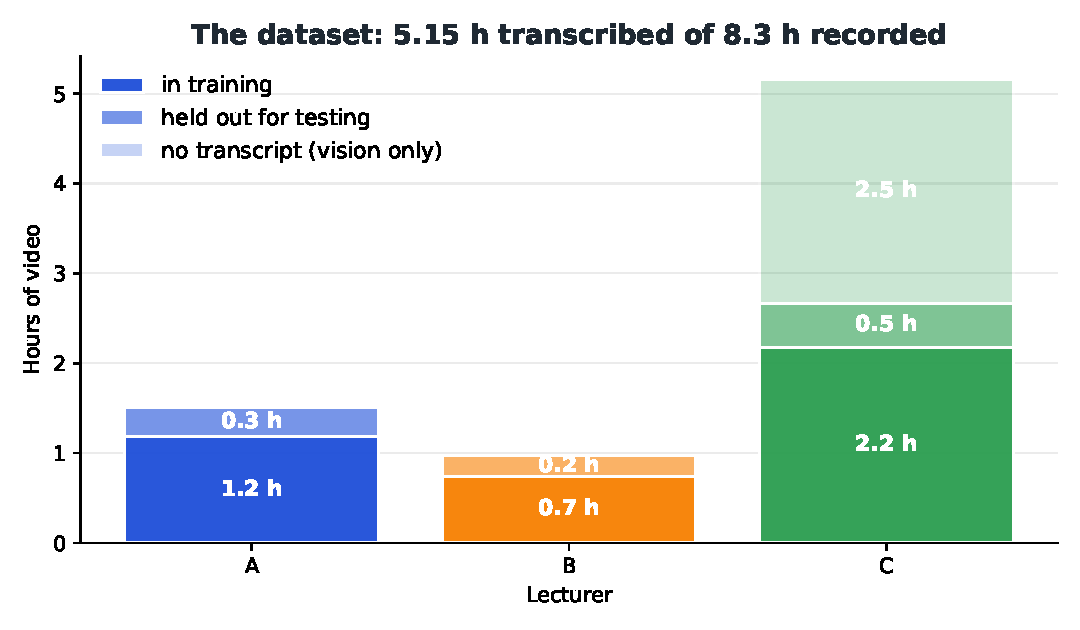
\includegraphics[width=0.85\textwidth]{fig-data-composition}
\caption{The corpus by lecturer. The darker part of each bar is training speech,
the middle part is held out for testing, and the lightest part is video with no
transcript, used for the vision side only.}
\label{fig:fig-data-composition}
\end{figure}

\begin{figure}[H]
\centering
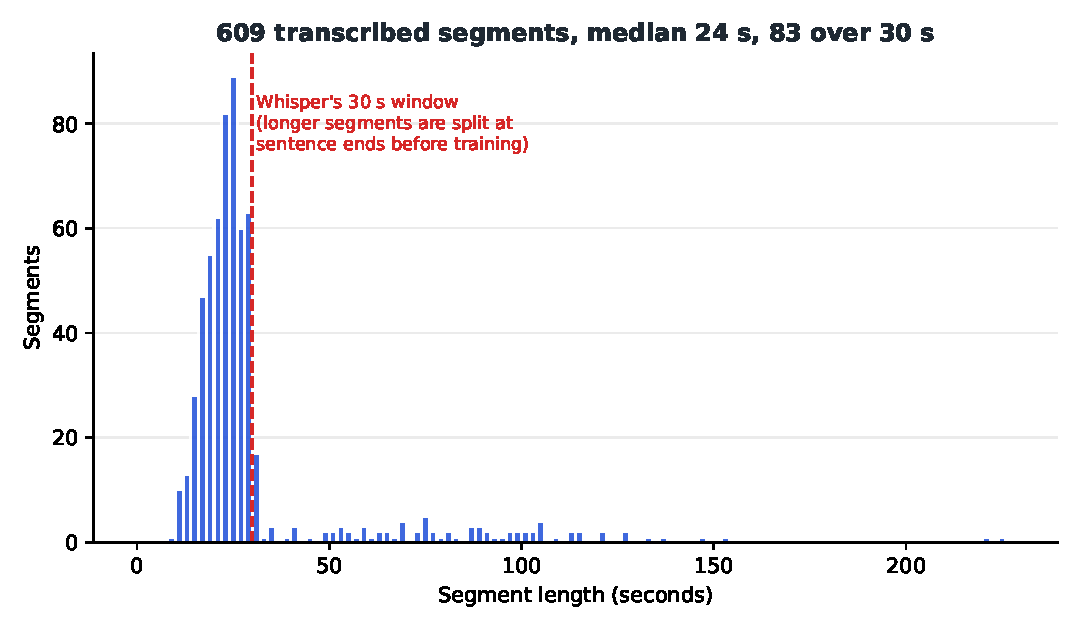
\includegraphics[width=0.85\textwidth]{fig-data-segments}
\caption{Lengths of the 609 transcribed segments against Whisper's 30 second
window. Segments longer than the window are subdivided at sentence ends before
training.}
\label{fig:fig-data-segments}
\end{figure}

\begin{figure}[H]
\centering
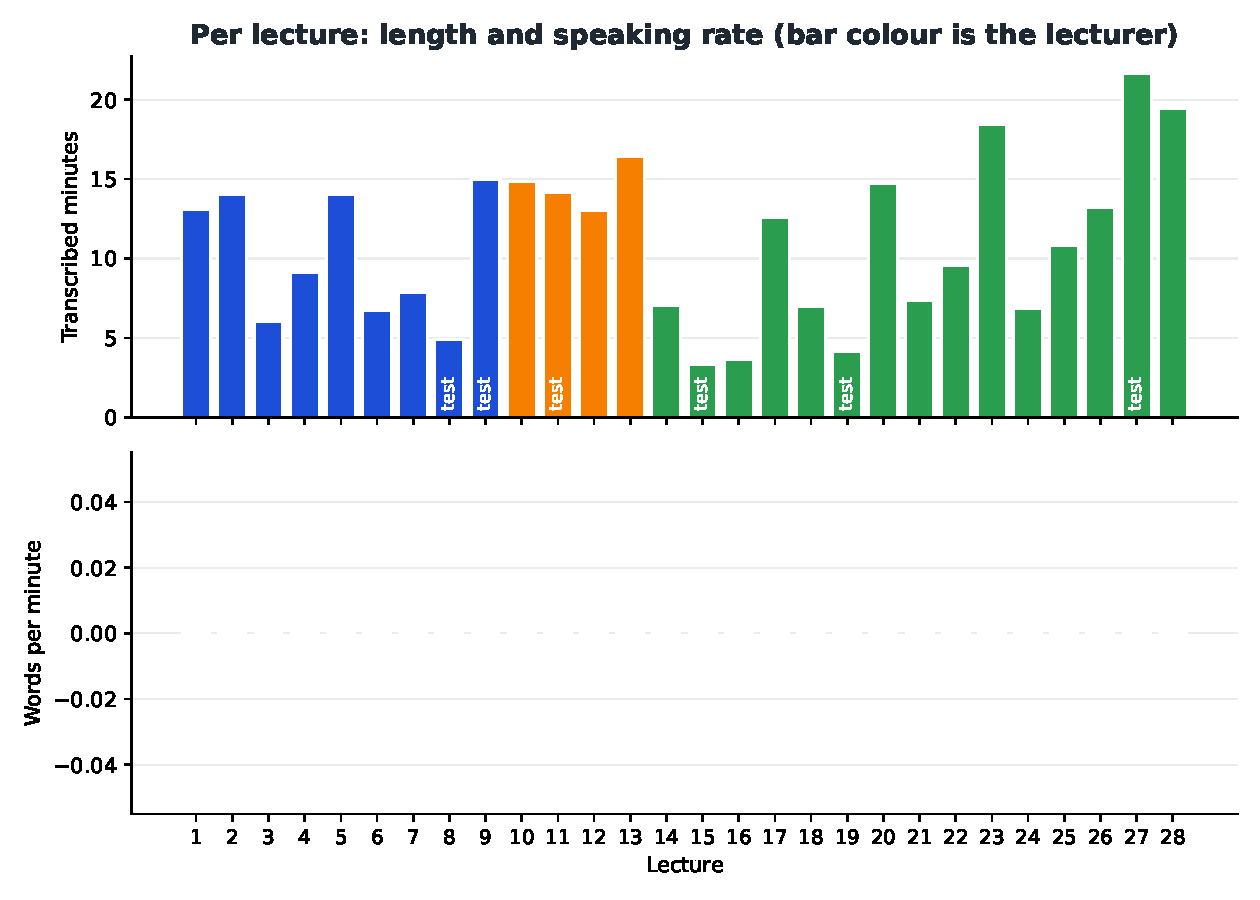
\includegraphics[width=\textwidth]{fig-data-per-lecture}
\caption{Transcribed minutes and speaking rate for each lecture with a transcript.
Bar colour is the lecturer. Lectures marked \textit{test} are the six held out for
the final result.}
\label{fig:fig-data-per-lecture}
\end{figure}

\begin{figure}[H]
\centering
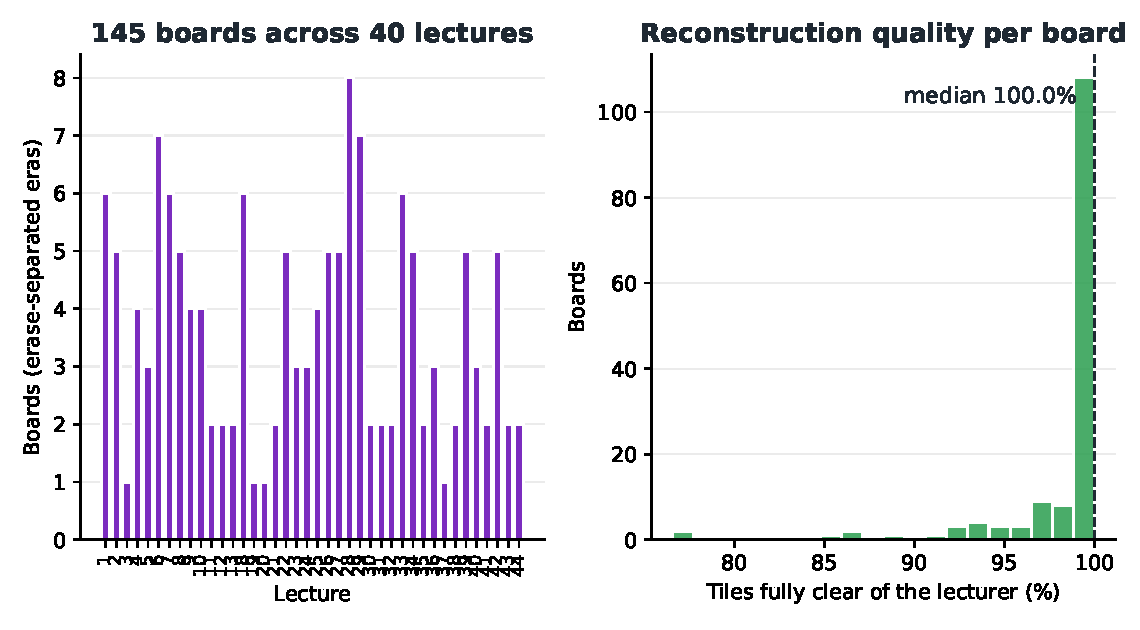
\includegraphics[width=\textwidth]{fig-data-boards}
\caption{Left, the number of erase-separated boards found in each lecture. Right,
the distribution of the fraction of tiles that found a completely clear view of
the board, with the median marked.}
\label{fig:fig-data-boards}
\end{figure}

\section{Implementation of Selected Design}

\subsection{Stage 1: adapting the speech model}

The base model is whisper-large-v3-turbo, an encoder-decoder transformer with 809
million parameters \cite{radford2023whisper}. The base weights are frozen. LoRA
adapters are attached to the query and value projection matrices of the attention
layers, with rank 16 and scaling factor alpha 32 \cite{hu2022lora}. Training uses a
batch size of 8, 8 epochs, bfloat16 precision, and gradient checkpointing on the
12 GB card, which cuts the memory needed from about 18 GB to 6.1 GB at the cost of
recomputing activations. Every run is done with two random seeds, 42 and 1, and both
are reported.

\textbf{Decoding.} The reported numbers use plain greedy decoding. The loop
safeguard from the Whisper paper is also available and is reported beside the main
result for comparison. It works by checking the gzip compression ratio of a
hypothesis, and if the ratio is above 2.4 the clip is decoded again with sampling at
temperatures 0.2, 0.4 and upwards until the output stops looping. It reads only the
hypothesis and never the reference, and it is applied identically to the base and
the adapted model. Only the compression ratio half of the published rule is used,
because the log probability half would resample most Banglish clips rather than only
the looping ones.

\subsection{Stage 1b: choosing the settings, and the pre-registered plan}

The panel question that any tuned result invites is whether the settings were
chosen by trying things until the test number looked good. The answer here is a
written plan, committed to version control before any tuning run, that fixes the
validation lectures, the order of the search, and the rule for accepting a winner.

The plan has five stages, run in order, each one starting from the winner of the
previous stage.

\begin{enumerate}
  \item \textbf{Learning rate}, over 5e-4, 1e-3 and 2e-3.
  \item \textbf{LoRA rank}, over 8, 16 and 32, with alpha fixed at twice the rank.
  \item \textbf{Which layers are adapted}, comparing the query and value
        projections against all four attention projections.
  \item \textbf{Number of epochs}, taken from the validation loss curve.
  \item \textbf{Seed stability}, by repeating the winner with a second seed.
\end{enumerate}

Everything else is held fixed, which means the base model, batch size 8, bfloat16,
gradient checkpointing and greedy decoding. The score is the median per-clip
character error rate on the validation clips. The acceptance rule is that a
candidate replaces the default only if it beats the default by more than the spread
between two seeds of the same configuration, which is the plan's way of refusing to
chase noise.

The procedure was run twice. A rehearsal on 2.69 hours of transcript was used to
check that the machinery worked, and the real run was repeated on the full corpus
once transcription closed. The second run supersedes the first, and Section 
ef{sec:asr-tuning}
reports both.

\subsection{Stage 2: reconstructing the board}

\textbf{Finding the eras.} The amount of ink on the board is tracked across frames.
When 30 per cent of it disappears between consecutive frames, the board has been
wiped, and the frames between two wipes form one era. An era shorter than four
frames is discarded.

\textbf{Tiling.} Work is done at a scan width of 640 pixels. The frame is cut into
tiles of 32 scan pixels with 50 per cent overlap between neighbours. A tile counts
as clear in a given frame when less than 2 per cent of it is covered by the
lecturer. For each tile independently, the pipeline takes the latest frame within
the era in which that tile was clear, and the chosen tiles are blended back together
with a raised-cosine weight so that the seams do not show.

This works because the lecturer occupies one place at a time. It is also the reason
the method has a stated limit, which is that it needs the lecturer to move. Where a
tile never finds a clear moment, the residue is left visible and reported rather
than filled in.

\textbf{Locating the lecturer.} Three options exist and the third is used. The
simplest takes whatever differs from the usual appearance of the board, which fails
when the lecturer stands still, because then he is part of the usual appearance, and
fails again when the camera's automatic exposure darkens a frame, because then every
pixel differs. The second uses a pretrained DeepLabV3 network with a ResNet-101
backbone and takes its person class frame by frame \cite{chen2017deeplabv3}. The
third adds a shadow mask to the network, computed as board that is darker than usual
after dividing out each frame's exposure gain, with pen-stroke-thin marks eroded away
so that writing is not mistaken for shadow. The third option recovers writing the
first one lost, including a diagram drawn at the end of an era and seven of the eight
digits of a binary number that the old mask reduced to four.

\textbf{Display clean-up.} A separate step flattens the background and fades
everything that is not clearly darker than its surroundings to white, in the manner
of the whiteboard mode of a document scanner application, and blanks the pixels the
mosaic itself flagged as the lecturer. This makes every board a clean white image.
It is important to be exact about what this step is, because it replaces background
pixels. A cleaned board is therefore not unmodified camera output. The strokes are
camera pixels and the background is not, and the report says so wherever a cleaned
board is shown. Section 
ef{sec:board-cleanup} reports the measured effect of this step on how well
the vision-language model reads the board, which was not the expected one.

\figplaceholder{fig-4-2-before-frame}{A single frame of the same lecture, showing
why one frame is not enough. The lecturer stands in front of the part of the board
he has just written on.}{Take one frame from
\texttt{output/lectures/BanglaASR29/frames/} where the lecturer is standing in
front of the writing, for example \texttt{frame\_000619\_001238s.jpg}, and blur or
pixelate his face before using it. The ethics statement says no person is
identifiable in the figures, so the face must be covered. Put it beside or above
the reconstructed board in Figure \ref{fig:board-mosaic-raw} if you prefer a
two-panel figure.}{6.5cm}

\begin{figure}[H]
\centering
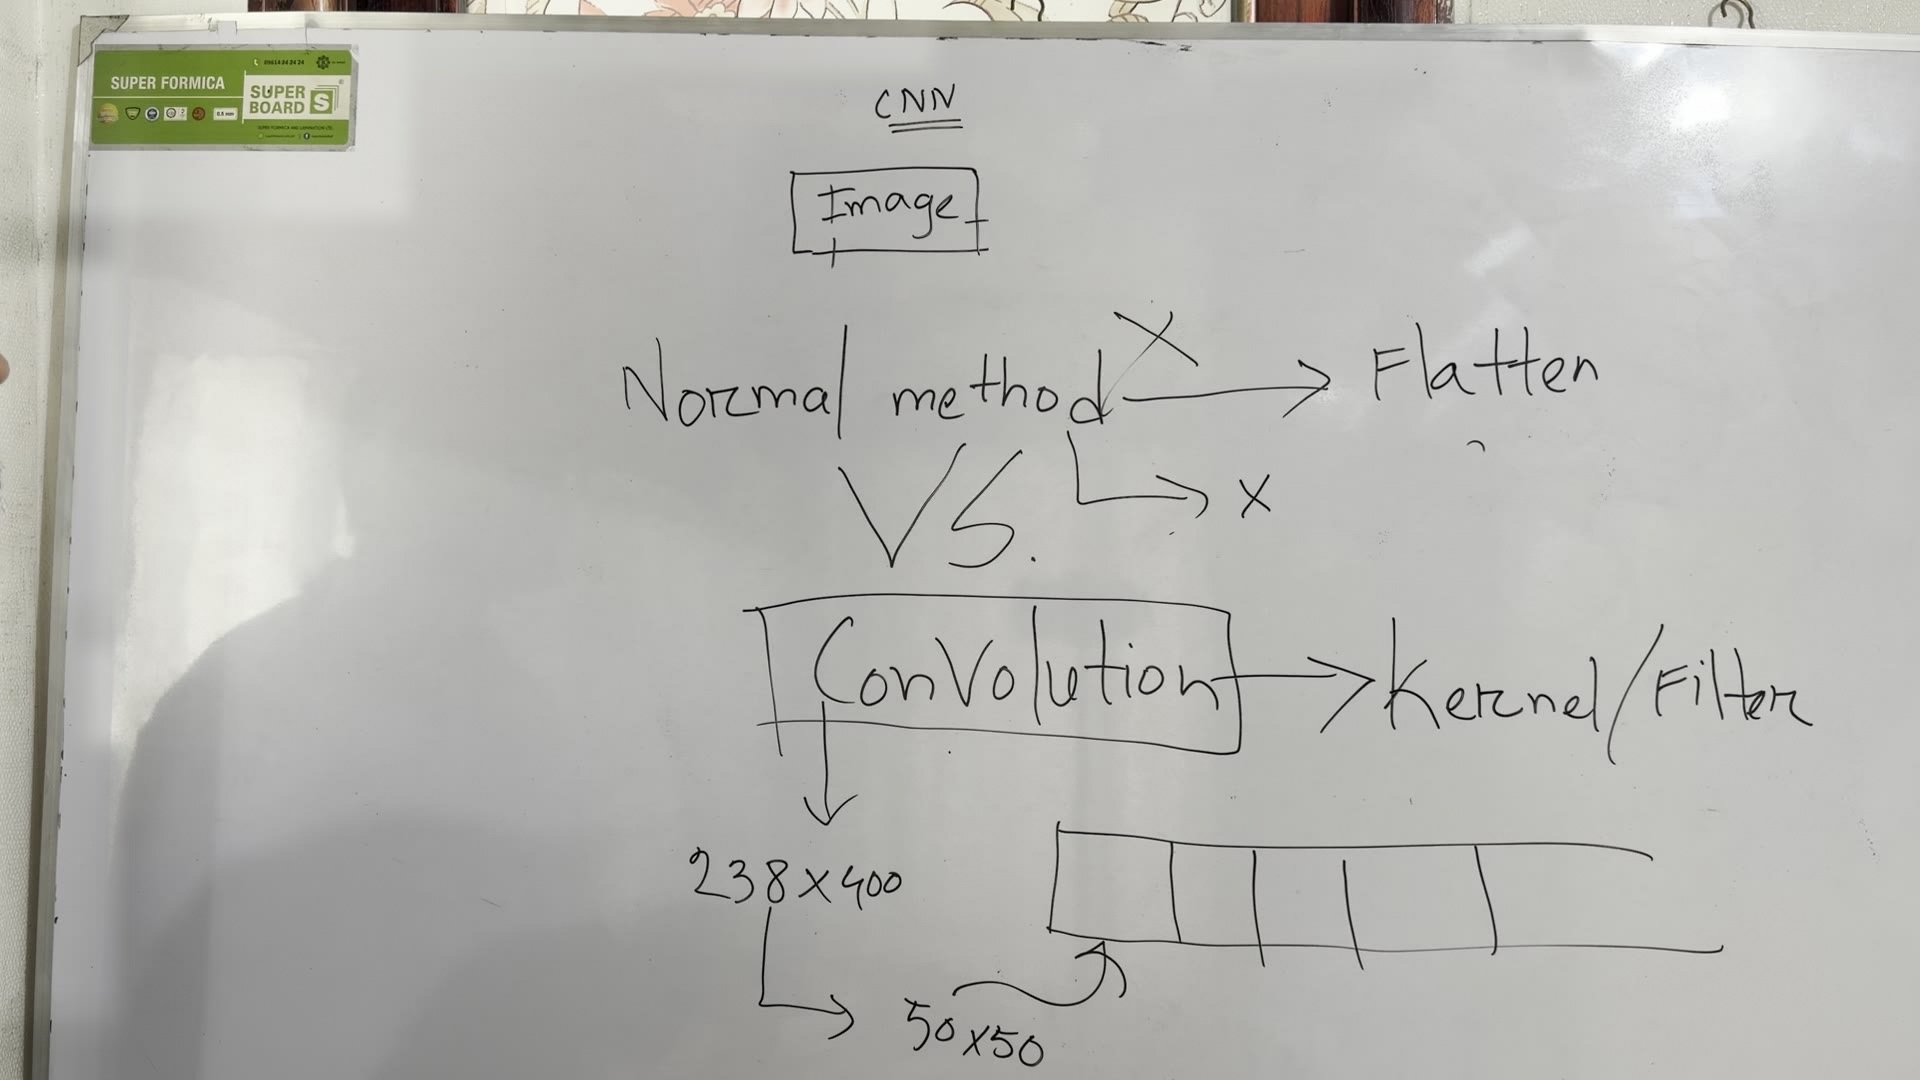
\includegraphics[width=0.92\textwidth]{board-mosaic-raw}
\caption{A reconstructed board from lecture BanglaASR29, era 5. Every pixel comes
from a real frame of the video. The lecturer stood in front of the left half of
this board for most of the era, and what remains of him is the soft grey shadow on
the left, not a filled-in guess.}
\label{fig:board-mosaic-raw}
\end{figure}

\begin{figure}[H]
\centering
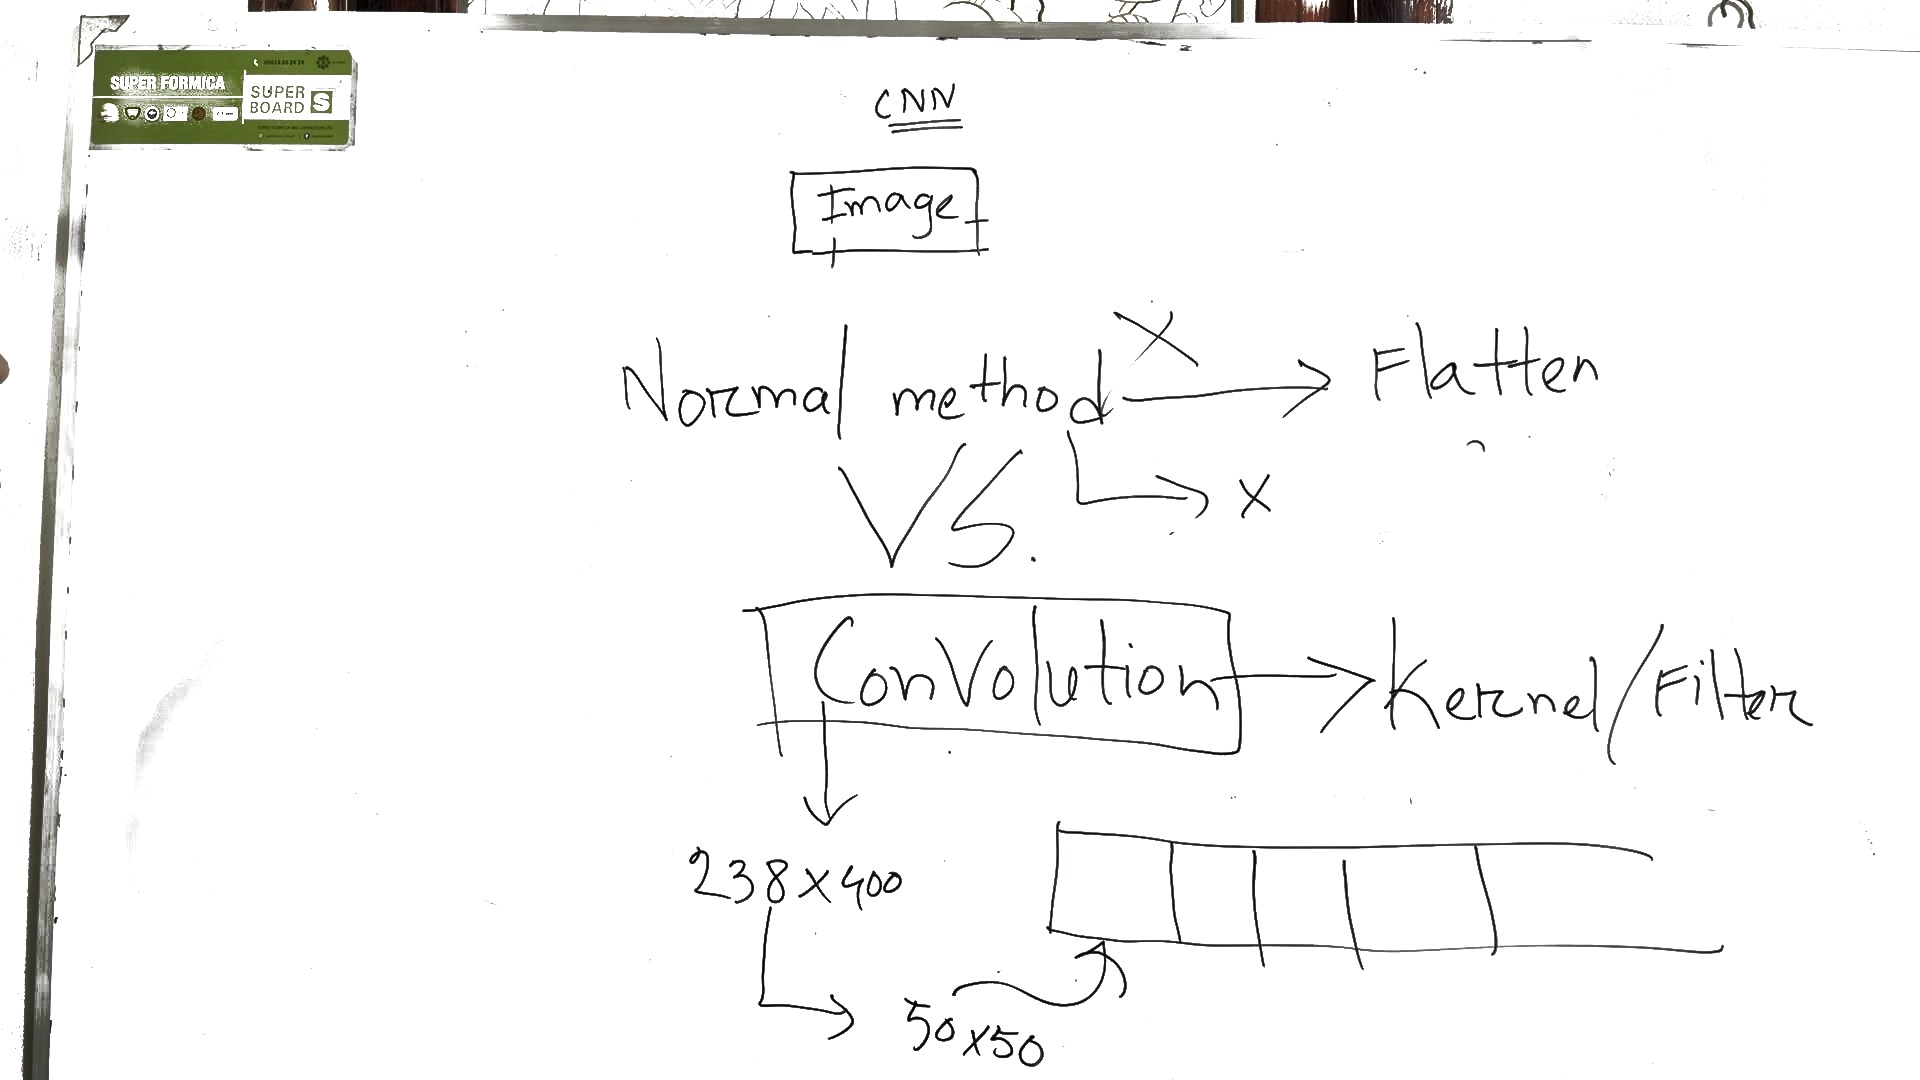
\includegraphics[width=0.92\textwidth]{board-mosaic-clean}
\caption{The same board after the display clean-up. The background has been
replaced, so this image is enhanced rather than unmodified camera output, while
the strokes themselves are camera pixels.}
\label{fig:board-mosaic-clean}
\end{figure}

\subsection{Stage 3: numbered boxes and the vision-language model}

\textbf{Finding the boxes.} Our own code, not the model, finds the blocks of
writing. It groups dark pixels, strips the board frame, drops specks by counting
dark pixels, and rejoins boxes that are parts of the same written line. At most ten
boxes are produced per board. Each box gets a number and a colour from a fixed list
of ten distinct colours, and the notes later refer to a box by both, for example
``the purple box 5''.

\textbf{Naming and transcribing.} The numbered boxes are drawn onto the clean board
and the image is given to Qwen2.5-VL-7B-Instruct with a prompt that asks, for each
numbered box, for a short name and a full transcription of what is inside it. This
is Set-of-Mark prompting \cite{yang2023som}, with the marks supplied by our code.
Boxes the model reports as empty are dropped.

Two defects in this stage were found during the real runs and both are handled in
code. On one board the model read the content correctly, then tried to draw a
diagonal line of the diagram and emitted the same backslash line 512 times, giving
42,037 characters. The reader now collapses a run of identical lines and records how
many it dropped, which matters because that text is pasted into the note prompt.
Separately, boards carrying code make the model emit unescaped quotation marks that
break the JSON it is asked to return, and without a fallback such a board loses all
of its boxes. A salvage parser now reads the identifier, name and text fields one at
a time when the JSON cannot be parsed.

\begin{figure}[H]
\centering
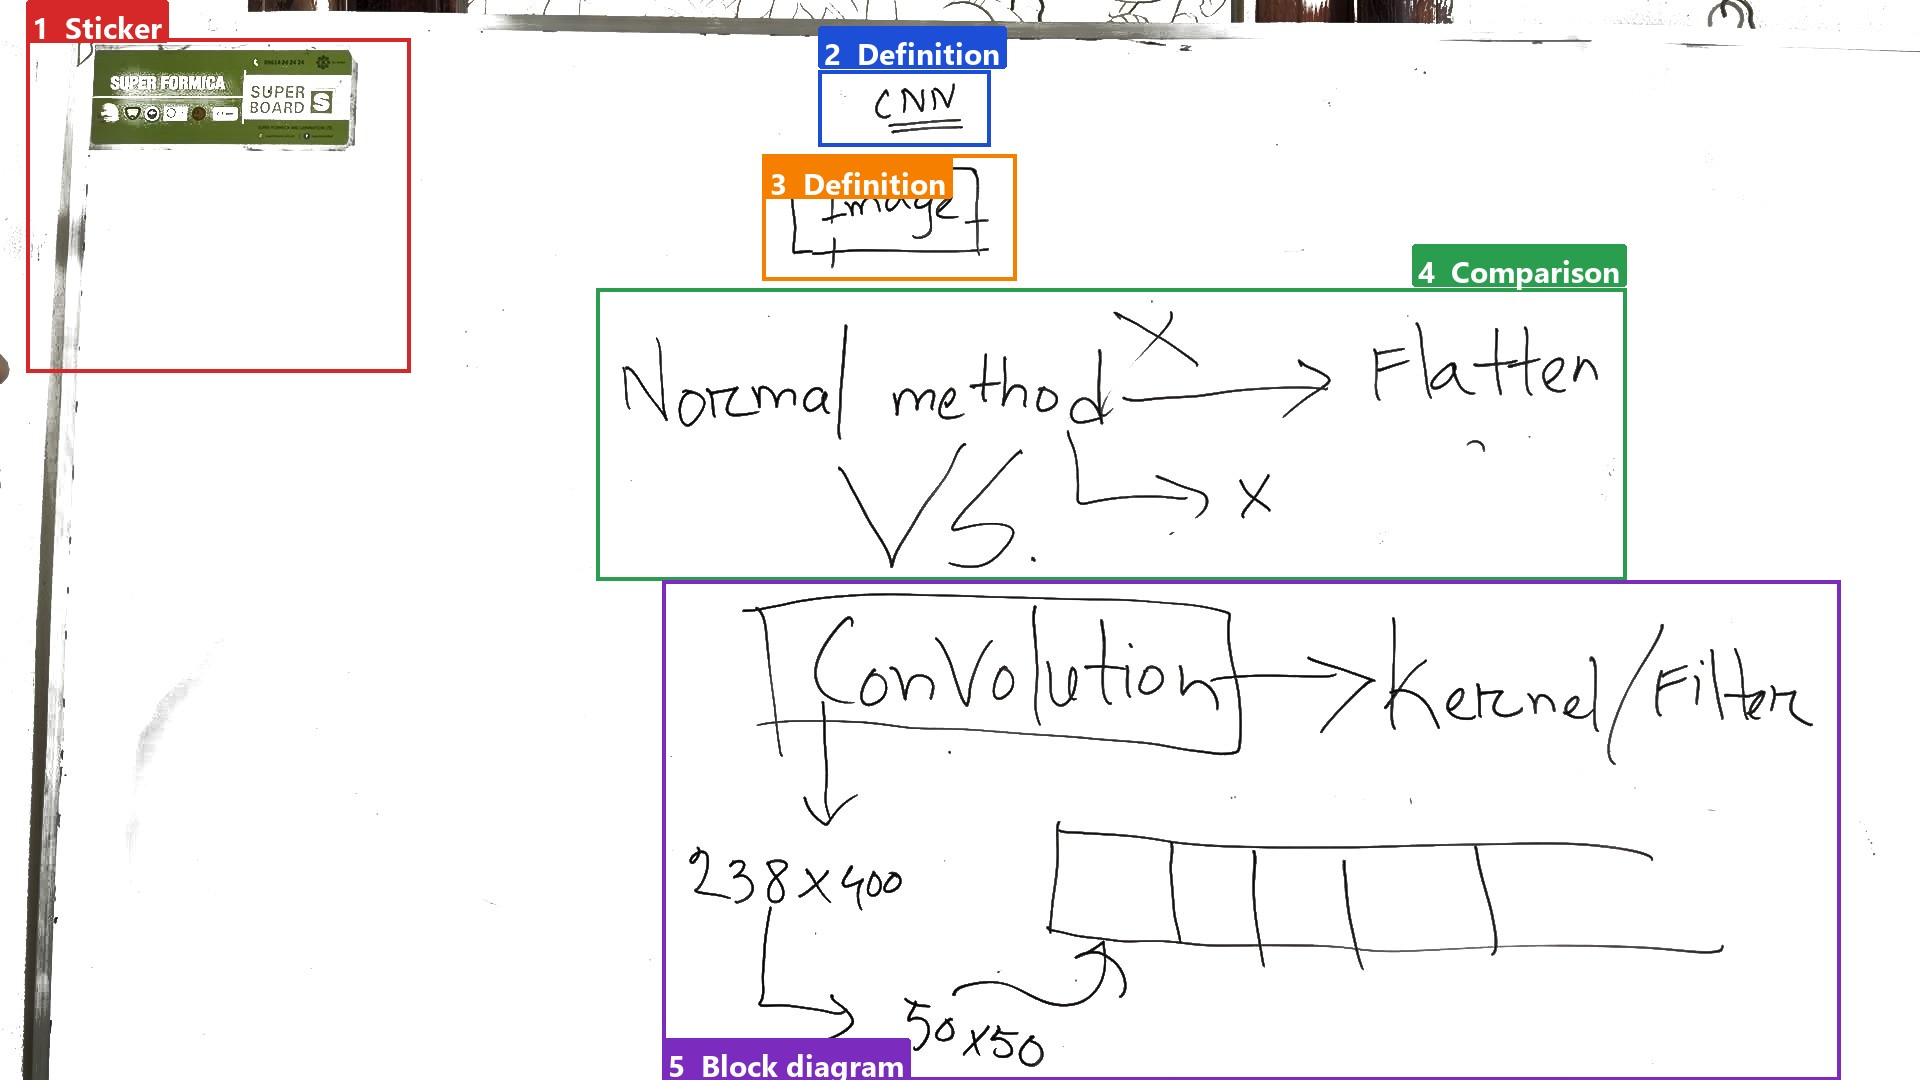
\includegraphics[width=0.92\textwidth]{board-demo-5}
\caption{The same board with the numbered coloured boxes drawn on it and named by
the vision-language model. The notes refer to these numbers and colours. Box 1 is a
manufacturer's sticker on the whiteboard, which the box finder treats as content
because it is dark and separate. This is a known cosmetic defect and is discussed in
Section 
ef{sec:known-defects}.}
\label{fig:board-demo-5}
\end{figure}

\subsection{Stage 4: writing the note}

The note is written by Qwen2.5-7B-Instruct, one call per board. Each call receives
the board image's boxes with their names and transcribed text, and the part of the
transcript that falls between that board's first and last frame, so that the model
sees the words that were spoken while that board was on the wall. A final call
produces the title, the takeaways and the self-check questions for the whole
lecture.

The prompt asks for a section that walks the reader through the board step by step,
refers to the boxes by number and colour, and quotes the lecturer between two and
five times. Material that is standard for the topic but that the lecturer did not say
is allowed, but only inside a section headed \texttt{Background}, which the page
builder renders as a dashed, labelled aside so that the reader can see it is not part
of the lecture. This is the controlled version of the failure that produced the wrong
textbook definition in the first version of the pipeline. The material is still
generated, but it is fenced and labelled instead of passing as something the lecturer
said.

Three checks then run over the generated text.

\textbf{The quote checker} takes every block quotation and searches for it in the
transcript. A quotation that is not there word for word is deleted, and the count of
kept and deleted quotations is written into the output file. A second counter flags
quoted spans of four or more words inside ordinary paragraphs that match neither the
transcript nor the board, but only flags them, because most of them turn out to be
code or translated lines rather than errors.

\textbf{The box reference check} removes any reference to a box number that the board
does not have, and counts them.

\textbf{The placeholder strip} removes the prompt's own example text when the model
copies it into the notes instead of leaving the quotation out. This was found by
reading the output, where the model had written the words \textit{exact words from
the transcript} as if they were a quotation.

\textbf{The two languages.} Each version is written wholly in its own language. The
Banglish note quotes the lecturer's real words, so the quote checker applies to it.
The English note quotes the lecturer in English translation, and a translation
cannot be matched against a Banglish transcript, so the checker does not run on the
English files. Every output file records which of the two it is, and Chapter 5 states
the resulting claim precisely, which is that quotations in the Banglish notes are
verified word for word and quotations in the English notes are unverified
translations.

The English note is produced by writing the section in Banglish first and then
translating it with the same model, keeping the Markdown structure, the tables, the
box numbers and the colours. A defect in this route was found and fixed. The
translation left 97 section labels in Banglish across the thirteen files, so a page
billed as English still showed Banglish headings, and three files returned the
summary line in capital letters. Both are repaired by a mapping script that does not
call the model, since the labels are a fixed set written by our own prompt. The
capitalisation repair takes each word's casing from how the same file writes that
word elsewhere, so that Python, TTL and DBMS survive.

\textbf{The page.} The sections are assembled into Markdown and into a single
self-contained HTML page with the board images embedded, coloured tags for the box
references and click-to-reveal answers for the self-check questions.

\subsection{How the system is run}

The whole pipeline is one command that takes a video and produces the notes. It runs
each stage as a separate process, skips any stage whose output already exists, and
writes the time each stage took to a JSON file beside the outputs. This is what makes
the run times in Section 3.3.2 measurements rather than estimates.

\subsection{Evaluation method}

Evaluation is described here once and is used throughout Chapter 5.

\textbf{Speech.} Word and character error rate are computed for each test clip
separately, and the median across clips is reported, because a single runaway output
can push a mean above 100 per cent. The base model and the adapted model are run on
exactly the same clips, so the comparison is paired and is tested with a Wilcoxon
signed-rank test and a sign test. The number of runaway clips is reported for both
models. Two spelling-tolerant variants are also computed. The first maps both sides
to the transcription guide's canonical spellings and collapses repeated vowels. The
second additionally counts a word as correct when it is at least 80 per cent similar
to the reference word, so that words of three letters or fewer still have to match
exactly. The rules for both were committed before any rescoring.

\textbf{Board reconstruction.} Two different things are counted and they must not be
confused. The fraction of tiles that found a completely clear view is computed by the
reconstruction itself and measures coverage, not whether writing survived. Whether
writing survived was answered by a person, who looked at each reconstructed board
beside two real frames from the same time and said whether anything written was
missing and what it was.

\textbf{Board reading and note quality.} Both are scored by recall of items from the
hand-verified answer keys. An answer key is a list of the things written on one
board, each labelled as a number, a name, a piece of code, a term or a phrase. Recall
is the right measure rather than F1, because good notes legitimately contain a great
deal that was not on the board, so precision would punish the behaviour we want.
Items of three characters or fewer must match as whole words, so that ``CS'' is not
found inside ``economics''. The keys were drafted from the board images and then
checked by hand, one board at a time, without the checker seeing any model output.
The folder holding them is refused by the note generator in code.

\textbf{Reporting rules.} Medians rather than means. The direction of every
difference is stated beside its p-value. Counting by board is reported alongside
counting by item, because the item count is dominated by a few dense boards and the
two can disagree. Results that go against the design are reported in the same detail
as results that support it.


\chapter{Result Analysis}
% ============================================================================
% CHAPTER 5 - RESULT ANALYSIS   (template file chapter_6.tex)
% Rubric mapping: CO6 (10 marks, 5 panel + 5 supervisor) is assessed from
% 5.1, 5.2, 5.3, 5.4, 5.5 and 5.6. CO7 (5 marks) is assessed from 5.3.
%
% EVERY number in this chapter comes from RESULTS.md in the project repository,
% where each one has the command that regenerates it.
% ============================================================================

\section{Performance Evaluation}

\subsection{What was measured, and the headline figures}

Each stage of the pipeline is evaluated on its own, because a single end-to-end
number would hide which part works. Table \ref{tab:headline} collects the main
results, and the rest of this section takes them one at a time.

\begin{table}[H]
\centering
\caption{The main results, one per stage. Each row has its own section below,
where the conditions and the caveats are stated.}
\label{tab:headline}
\small
\begin{tabular}{p{4.0cm}p{4.4cm}p{5.0cm}}
\toprule
\textbf{Stage} & \textbf{Measure} & \textbf{Result} \\
\midrule
Speech, six unseen lectures &
Median per-clip character error rate &
\textbf{67.7\% to 15.8\%} and 16.0\% in two seeds \\
\addlinespace
Speech, unseen lecturer &
Median per-clip character error rate &
72.8\% to 50.3\%, all six runs significant \\
\addlinespace
Board reconstruction &
Tiles finding a clear view, 35 boards &
median 97.7\% \\
\addlinespace
Board reconstruction &
Human check, 98 boards &
82 complete, 9 with writing genuinely lost \\
\addlinespace
Board reading &
Recall of 349 hand-verified items &
\textbf{31.2\% to 88.8\%} by changing the prompt \\
\addlinespace
Generated notes &
Recall of 349 hand-verified items &
\textbf{37.2\% to 89.1\%} \\
\bottomrule
\end{tabular}
\end{table}

\subsection{Speech recognition: the final result}
\label{sec:asr-result}

The corpus was closed at 28 transcripts and 5.15 hours. Whole lectures were held
out at random, 20 per cent of each lecturer's minutes with the seed fixed at zero,
giving 22 training lectures totalling 4.10 hours and six test lectures totalling
1.05 hours and 177 clips. The three validation lectures used for tuning were locked
out of the test set. Table \ref{tab:asrfinal} gives the result.

\begin{table}[H]
\centering
\caption{Median per-clip error on the 177 test clips, off-the-shelf against
fine-tuned. Greedy decoding throughout. The last row is the same configuration as
the row above it with a different random seed.}
\label{tab:asrfinal}
\small
\begin{tabular}{p{2.6cm}p{1.2cm}p{1.4cm}p{1.4cm}p{2.0cm}p{1.8cm}p{1.8cm}}
\toprule
\textbf{Learning rate} & \textbf{Seed} & \textbf{CER} & \textbf{WER} &
\textbf{Runaway clips} & \textbf{Better of 177} & \textbf{Wilcoxon} \\
\midrule
off-the-shelf & -- & 67.7\% & 93.9\% & 13 & -- & -- \\
\textbf{1e-3} & \textbf{42} & \textbf{15.8\%} & \textbf{42.5\%} & 1 & 164 &
p $<$ 1e-30 \\
\textbf{1e-3} & \textbf{1} & \textbf{16.0\%} & \textbf{41.7\%} & 1 & 167 &
p $<$ 1e-30 \\
2e-3 (the tuned choice) & 1 & 16.2\% & 41.7\% & 2 & 168 & p $<$ 1e-30 \\
2e-3 (the tuned choice) & 42 & \textbf{118.7\%} & 189.8\% & \textbf{82} & 35 &
worse \\
\bottomrule
\end{tabular}
\end{table}

The headline is that the character error rate falls from 67.7 per cent to 15.8 and
16.0 per cent, and the word error rate from 93.9 per cent to 42.5 and 41.7 per
cent. Two seeds agree to within 0.2 points, and the fine-tuned model is better on
164 and 167 of the 177 clips. About three quarters of the character error is
removed.

\begin{figure}[H]
\centering
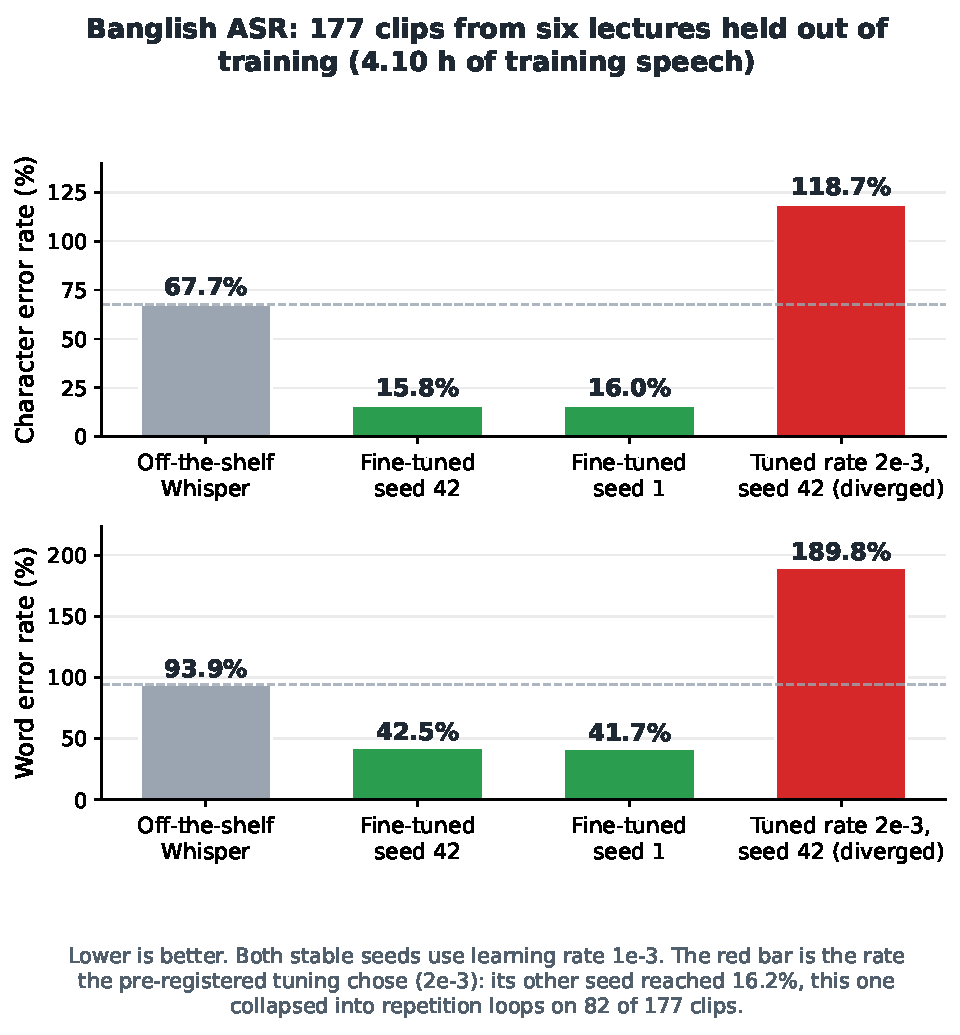
\includegraphics[width=0.9\textwidth]{fig-asr-final}
\caption{The final speech result. Median per-clip error before and after
fine-tuning, for both stable seeds, with the diverged seed shown beside them
rather than left out.}
\label{fig:fig-asr-final}
\end{figure}

\begin{figure}[H]
\centering
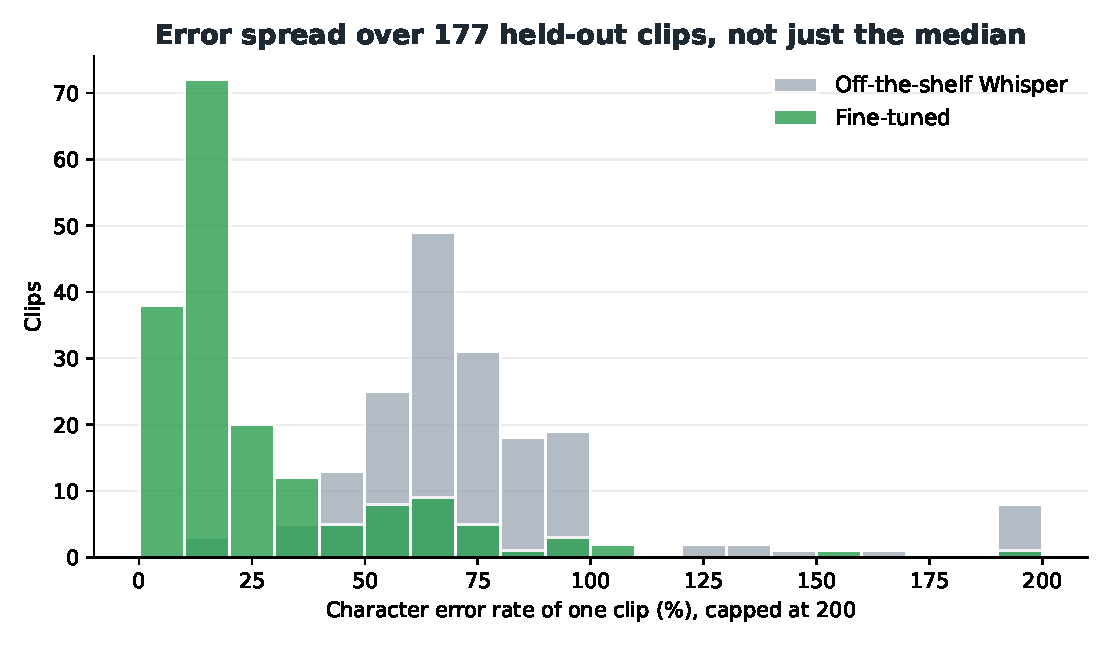
\includegraphics[width=0.9\textwidth]{fig-asr-distribution}
\caption{The distribution of per-clip character error rate over the 177 test
clips, before and after fine-tuning. The shift is of the whole distribution, not
of a few easy clips.}
\label{fig:fig-asr-distribution}
\end{figure}

\begin{figure}[H]
\centering
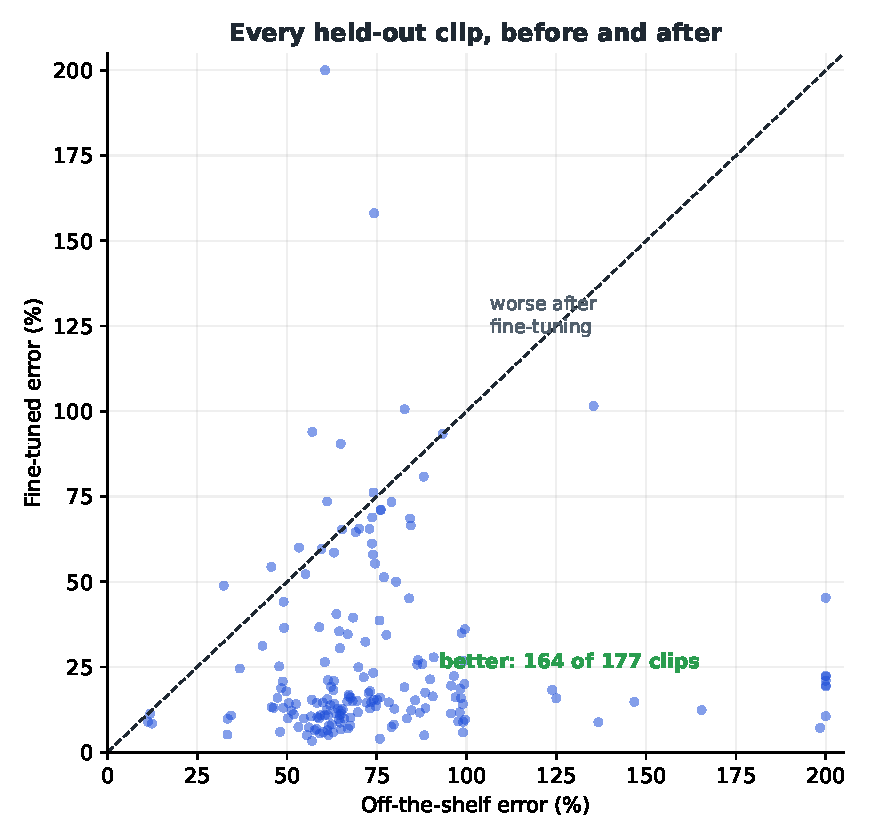
\includegraphics[width=0.9\textwidth]{fig-asr-clip-scatter}
\caption{Each point is one test clip, with its error before fine-tuning on one
axis and after on the other. Points below the diagonal improved. The clips at the
extreme right are the ones where the off-the-shelf model fell into a repetition
loop.}
\label{fig:fig-asr-clip-scatter}
\end{figure}

\textbf{The instability, which has to be reported with the result.} At 2e-3, which
is the learning rate the pre-registered procedure chose on the validation
lectures, one of the two seeds collapsed. It produced runaway output on 82 of the
177 clips and a character error rate of 118.7 per cent, which is worse than doing
nothing at all. The data, the split and every other setting were identical to the
seed that reached 16.2 per cent. The 16.2 per cent figure is therefore never quoted
in this thesis without its failed twin.

This is not the first time this configuration has shown the same fragility. LoRA
rank 32 diverged and adapting all four attention projections diverged, in both the
rehearsal and the full tuning run, which is reported in the next section.

\textbf{A disclosure about the 1e-3 rows.} The pre-registered procedure selected
2e-3. The runs at 1e-3 were launched after the divergence at 2e-3 had been seen, so
that choice was not blind, and the thesis says so rather than presenting 1e-3 as
the pre-registered winner. What can be claimed honestly is narrower and is still
worth claiming. The runner-up rate from the same tuning table is stable across two
seeds on the test set and its two seeds agree to 0.2 points, while the chosen rate
is not stable. The selection rule itself was not changed and remains recorded in
the committed tuning plan.

\subsection{How the training settings were chosen}
\label{sec:asr-tuning}

The tuning procedure of Section 4.4.2 was run on the full corpus, scored only on
the three validation lectures, and never on the test lectures. Off-the-shelf
Whisper on those validation clips gives a character error rate of 73.8 per cent and
a word error rate of 97.6 per cent. Table \ref{tab:tuning} is the result.

\begin{table}[H]
\centering
\caption{Pre-registered hyperparameter tuning on the full corpus, scored on the
three validation lectures. Each stage starts from the winner of the previous one.
The rows marked as diverged produced output worse than the off-the-shelf model.}
\label{tab:tuning}
\small
\begin{tabular}{p{2.9cm}p{2.3cm}p{1.1cm}p{1.0cm}p{1.4cm}p{1.1cm}p{1.2cm}p{1.2cm}}
\toprule
\textbf{Stage} & \textbf{Run} & \textbf{lr} & \textbf{rank} & \textbf{layers} &
\textbf{epochs} & \textbf{val CER} & \textbf{val WER} \\
\midrule
1 learning rate & lr 5e-4 & 5e-4 & 16 & q,v & 8 & 37.9\% & 60.0\% \\
1 learning rate & lr 1e-3 (default) & 1e-3 & 16 & q,v & 8 & 42.2\% & 61.9\% \\
1 learning rate & \textbf{lr 2e-3} & 2e-3 & 16 & q,v & 8 & \textbf{33.6\%} &
\textbf{54.5\%} \\
2 LoRA rank & rank 8 & 2e-3 & 8 & q,v & 8 & 40.1\% & 64.1\% \\
2 LoRA rank & rank 32 & 2e-3 & 32 & q,v & 8 & \textbf{126.6\% diverged} &
200.0\% \\
3 adapted layers & all four projections & 2e-3 & 16 & q,k,v,o & 8 &
\textbf{134.7\% diverged} & 174.4\% \\
4 epochs & 5 epochs & 2e-3 & 16 & q,v & 5 & 39.4\% & 59.6\% \\
5 stability & seed 1 & 2e-3 & 16 & q,v & 8 & 39.1\% & 59.6\% \\
\bottomrule
\end{tabular}
\end{table}

The procedure chose a learning rate of 2e-3, rank 16, the query and value
projections and 8 epochs. That configuration is 8.6 character error points better
than the starting point, and the acceptance rule required it to beat the default by
more than the spread between two seeds, which here is 5.4 points.

Three findings come out of this table, and none of them is flattering.

\textbf{More adapter capacity hurts at this learning rate.} Rank 32 diverged
outright, and adapting all four attention projections diverged as well. More
trainable parameters are not better here. Five hours of speech does not support
them.

\textbf{Validation loss is a poor guide to the metric that is reported.} The
validation loss is lowest at 5 epochs, at 1.666 against 1.801 at 8 epochs, so stage
4 retrained there. The character error rate got worse, from 33.6 to 39.4 per cent.
The lesson, which is worth stating because it is a common mistake, is to select on
the metric that will be reported rather than on the loss.

\textbf{The margin is not large next to seed noise.} The winner is 8.6 points ahead
of the default with a 5.4 point spread from a single seed change, measured on 34
minutes of validation speech. It passes the rule that was written down in advance,
and it is still a modest effect. The outcome on the test set, where that same
configuration diverged on one seed, is consistent with a genuinely noisy region of
the setting space rather than with a clear winner.

A rehearsal of the same procedure had been run earlier on 2.69 hours of transcript,
while transcription was still going on, to check that the machinery worked. It
chose the same learning rate, and it produced the same two divergences at rank 32
and at four projections. Its full table is in the project record.

\subsection{Decoding, and the loop safeguard}
\label{sec:asr-safeguard}

An earlier result in this project, on a smaller model, only beat its baseline when
Whisper's compression-ratio loop safeguard was switched on. The obvious challenge to
the present result is therefore that the safeguard is doing the work. It is not.
Table \ref{tab:safeguard} rescored both final models with the safeguard on.

\begin{table}[H]
\centering
\caption{The final model scored with plain greedy decoding and with Whisper's loop
safeguard. The safeguard is applied identically to both models and reads only the
hypothesis.}
\label{tab:safeguard}
\small
\begin{tabular}{p{2.0cm}p{2.6cm}p{3.4cm}p{4.4cm}}
\toprule
\textbf{Seed} & \textbf{Greedy CER} & \textbf{With the safeguard} &
\textbf{Runaway clips, greedy} \\
\midrule
42 & 15.8\% & 15.8\% & 1 of 177 \\
1 & 16.0\% & 16.0\% & 1 of 177 \\
\bottomrule
\end{tabular}
\end{table}

The two are identical to the first decimal place, because the fine-tuned model loops
on one clip in 177 and the safeguard has nothing to rescue. Off-the-shelf Whisper
loops on thirteen. All figures reported in this thesis are the plain greedy ones.

\subsection{Where the gain is uneven}
\label{sec:asr-perlecture}

The improvement is not evenly spread, and the pattern follows the training data.
Table \ref{tab:perlecture} breaks the result down by test lecture.

\begin{table}[H]
\centering
\caption{Median character error rate per test lecture, seed 42, with the amount of
that lecturer's speech in the training set.}
\label{tab:perlecture}
\small
\begin{tabular}{p{2.8cm}p{2.0cm}p{1.4cm}p{2.4cm}p{2.0cm}p{2.6cm}}
\toprule
\textbf{Test lecture} & \textbf{Lecturer} & \textbf{Clips} &
\textbf{Off-the-shelf} & \textbf{Fine-tuned} &
\textbf{That lecturer in training} \\
\midrule
BanglaASR8 & A & 14 & 68\% & 15\% & 1.2 h \\
BanglaASR9 & A & 41 & 67\% & 12\% & 1.2 h \\
\textbf{BanglaASR11} & \textbf{B} & 46 & 70\% & \textbf{52\%} & \textbf{0.7 h} \\
BanglaASR15 & C & 8 & 88\% & 12\% & 2.2 h \\
BanglaASR19 & C & 12 & 65\% & 12\% & 2.2 h \\
BanglaASR27 & C & 56 & 73\% & 16\% & 2.2 h \\
\bottomrule
\end{tabular}
\end{table}

\begin{figure}[H]
\centering
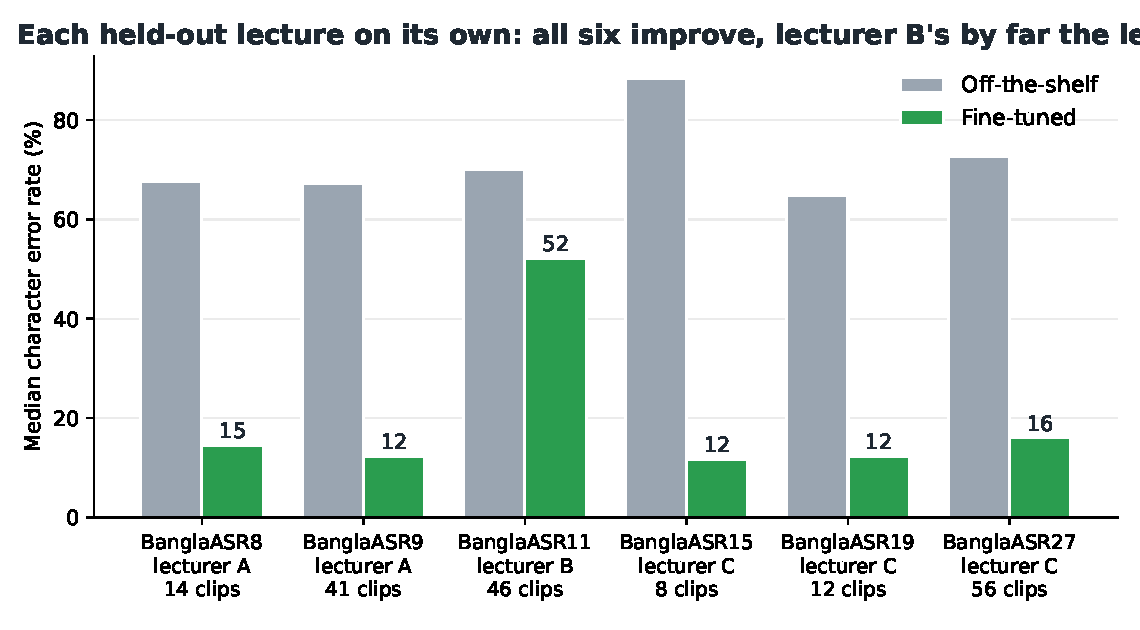
\includegraphics[width=\textwidth]{fig-asr-per-lecture}
\caption{Median character error rate for each test lecture before and after
fine-tuning. Every lecture improves. Lecturer B's lecture improves least, and
lecturer B contributed the least training speech.}
\label{fig:fig-asr-per-lecture}
\end{figure}

Every lecture improves, but lecturer B's lecture improves by far the least, ending
at 52 per cent where the others reach 12 to 16 per cent, and lecturer B contributed
the least training speech at 0.7 hours. With one test lecture per lecturer at the
low end, this is an observation and not a controlled result. It cannot separate
``less data from this lecturer'' from ``this lecturer is harder to transcribe''.
The honest reading is that it is the most likely explanation and the clearest
argument for collecting more speech from under-represented lecturers.

\subsection{Is the remaining error only a spelling problem?}
\label{sec:asr-spelling}

Banglish has no standard spelling, so a reasonable challenge is that the word error
rate is inflated by \textit{aami} against \textit{ami}. Two spelling-tolerant
variants were computed on the same saved outputs, with the rules committed before
any rescoring, and are shown in Table \ref{tab:spelling}. These numbers come from
the six leave-one-speaker-out runs rather than from the final model, because that
was the headline at the time the rules were fixed.

\begin{table}[H]
\centering
\caption{Spelling-tolerant word error rates, mean of six per-run medians. nWER maps
both sides to the transcription guide's canonical spellings and collapses repeated
vowels. fWER additionally accepts a word at 80 per cent character similarity, so
words of three letters or fewer must still match exactly.}
\label{tab:spelling}
\small
\begin{tabular}{p{5.0cm}p{3.0cm}p{3.0cm}}
\toprule
\textbf{Measure} & \textbf{Base} & \textbf{Fine-tuned} \\
\midrule
Plain word error rate & 95.3\% & 75.7\% \\
Spelling-fair nWER & 95.0\% & 74.8\% \\
Fuzzy fWER & 92.7\% & 68.2\% \\
\bottomrule
\end{tabular}
\end{table}

The canonical spelling table moves the word error rate by about one point, and
accepting near-miss spellings moves it by about seven more. Most of the word error
is therefore genuine recognition error rather than spelling disagreement. The
fine-tuned model is better in all six runs on all three measures, with p between
2.2e-16 and 2.7e-06. Plain word and character error rates remain the headline, and
this table exists to answer the spelling question when it is asked.

\subsection{An unseen lecturer, and a correction to an earlier result}
\label{sec:asr-loso}

The result in Section \ref{sec:asr-result} holds out whole lectures from lecturers
who are also heard in training. A harder question is what happens on a lecturer the
model has never heard. Each lecturer was held out in turn and the model trained on
the other two, with two seeds per fold and plain greedy decoding.

\begin{table}[H]
\centering
\caption{Leave-one-speaker-out. Each row holds out one lecturer entirely.}
\label{tab:loso}
\small
\begin{tabular}{p{2.4cm}p{2.6cm}p{3.2cm}p{3.2cm}p{2.0cm}}
\toprule
\textbf{Held out} & \textbf{Trained on} &
\textbf{WER, base to tuned} & \textbf{CER, base to tuned} &
\textbf{Wilcoxon} \\
\midrule
A, 172 clips & B + C, 82.9 min & 97.5\% to 76.2 / 75.8\% &
74.2\% to 51.8 / 49.9\% & p $<$ 1e-10 \\
B, 184 clips & A + C, 80.0 min & 93.8\% to 73.5 / 74.8\% &
70.0\% to 48.8 / 52.1\% & p $<$ 1e-08 \\
C, 75 clips & A + B, 114.0 min & 94.6\% to 74.5 / 79.8\% &
74.2\% to 45.2 / 54.0\% & p $<$ 1e-05 \\
\bottomrule
\end{tabular}
\end{table}

Averaged over the six runs, the character error rate falls from 72.8 per cent to
50.3 per cent and the word error rate from 95.3 per cent to 75.7 per cent. All six
runs are significant under plain decoding, and runaway clips fall or stay level in
every fold.

What this supports is that fine-tuning on 80 to 114 minutes of transcribed Banglish
from two lecturers cuts the character error on a third, unheard lecturer by about a
third, for every one of the three lecturers and in both seeds. What it does not
support is that this is usable speech recognition, since a 50 per cent character
error rate is still very high, or that the finding holds across many speakers, since
three is a small number.

Both designs belong in the thesis and both are labelled every time they appear. The
result in Section \ref{sec:asr-result} is ``new lectures from known lecturers'' on
4.10 hours of training speech, and this one is ``an unseen lecturer'' on 80 to 114
minutes.

\textbf{A correction that has to be recorded.} An earlier version of this work
reported a word error rate falling from 96.1 to 81.8 per cent on a speaker never
seen in training. That claim was wrong, and the reason is instructive. The original
nine transcripts carried no lecturer label, so the lectures were labelled by hand,
and one lecture was attributed to the wrong lecturer. That lecture was in the
training set and its lecturer was the test speaker, so 47 clips of the supposedly
unseen speaker had been trained on. The error was found by computing speaker
embeddings, which separate the groups without ambiguity at 0.99 to 1.00 similarity
within a lecturer and 0.75 to 0.80 across. The result was recomputed on the
corrected split, the old number was retired, and the voice check is now a standing
part of the data preparation. This is also the reason the corpus statistics in
Chapter 4 report the lecturer of every recording from voice rather than from a file
name.

\textbf{A data quality check on the same result.} Nine of 156 timestamps in the
ground truth behind these runs carried stray spaces, so their text joined the
previous segment and ten test clips carried more words than their audio. Both models
were scored on the same clips, so the comparison is fair, but the effect was measured
rather than assumed. Without those ten clips the result is 72.2 per cent to 49.6 per
cent character error, against the published 72.8 to 50.3. The defect made the
published figure slightly pessimistic, so the published figure stands.

\subsection{Board reconstruction: coverage}
\label{sec:board-coverage}

The reconstruction is measured first by coverage, which is the fraction of tiles
that found a moment when the lecturer was not in front of them. Across the 35
boards of the first nine lectures, the median board has 97.7 per cent of its tiles
fully clear, the mean is 96.5 per cent, and the range is 87.5 to 100 per cent. Six
boards reach 100 per cent, 26 of the 35 reach 95 per cent or better, and only two
fall below 90 per cent. Over all 145 boards produced in the project the median is
100 per cent and the mean 98.4 per cent, with the worst board at 76.6 per cent.

Two things drive the weak boards. Short eras give a tile fewer chances to be seen
clear, and six eras are under eight frames. A lecturer who stands in one place is
the other cause, and the worst lecture in the set is the one where the lecturer holds
a single position far longer than the others.

That second cause was addressed rather than excused. For the lecturer who moves
least, extracting frames every 2 seconds instead of every 10 gives each tile five
times as many chances. The number of his boards reaching 95 per cent clear rose from
1 to 5 out of 10, and the worst board improved from 59 to 88 per cent.

Coverage is a measure of the method, not of the result, and it is important not to
read it as fidelity. A tile can be clear and the writing can still be missing,
because the writing may never have been visible in any frame. That question needs a
person, and it is the next section.

\subsection{Board reconstruction: what a human check found}
\label{sec:board-human}

Every one of the 98 boards of the newer lectures was checked by hand. A page showed
each reconstructed board beside two real frames from the same period of the video,
and the question was whether the board contains everything that was written. Table
\ref{tab:completeness} gives the answers.

\begin{table}[H]
\centering
\caption{Human check of 98 reconstructed boards.}
\label{tab:completeness}
\small
\begin{tabular}{p{6.0cm}p{2.0cm}p{5.4cm}}
\toprule
\textbf{Verdict} & \textbf{Boards} & \textbf{} \\
\midrule
\textbf{Complete} & \textbf{82} & 83.7 per cent of 98 \\
Something missing & 16 & \\
\quad writing genuinely lost & 9 & 9.2 per cent \\
\quad era cut while the board was being wiped & 4 &
the board is half erased in every frame of that era \\
\quad camera out of focus for the whole era & 3 &
unreadable in the source video, not a reconstruction fault \\
\bottomrule
\end{tabular}
\end{table}

\begin{figure}[H]
\centering
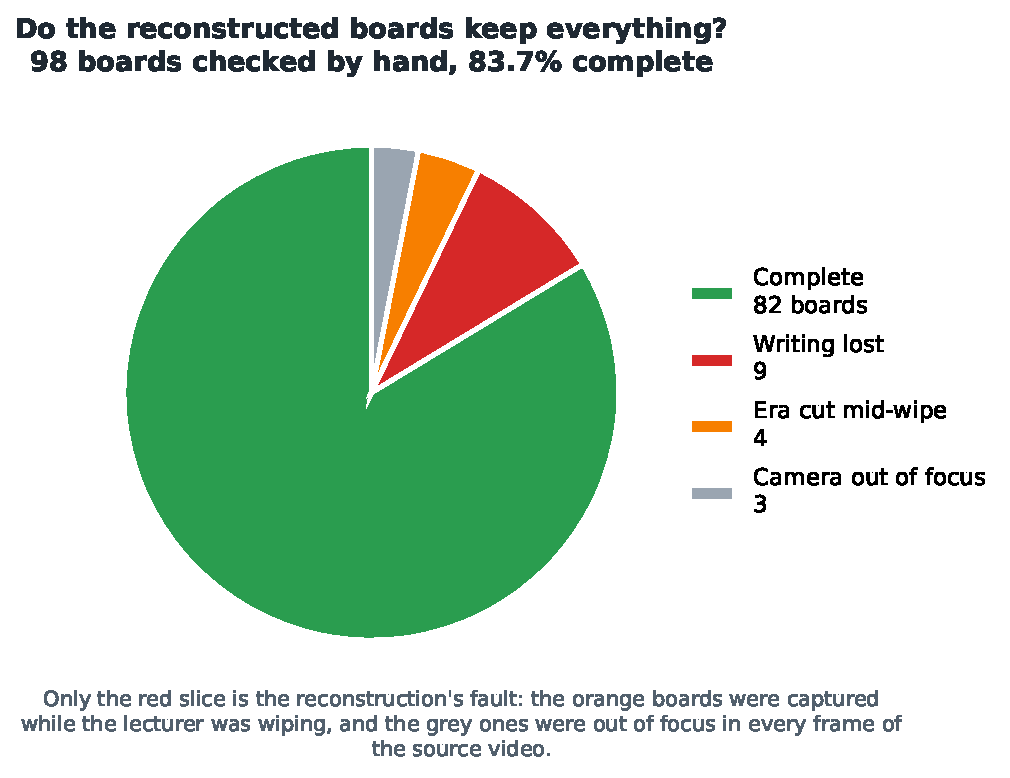
\includegraphics[width=0.9\textwidth]{fig-board-completeness}
\caption{The human check of 98 reconstructed boards, with the causes of the
sixteen incomplete ones separated.}
\label{fig:fig-board-completeness}
\end{figure}

The nine real losses are small. Seven of them are a single token or one diagram,
such as a label \texttt{t4}, the number \texttt{100} or the word Hybrid. One board
is the bad case, where a whole subnetting tree is absent. Counting only the boards
whose source frames were usable, which means dropping the four mid-erase eras and
the three out-of-focus ones, the reconstruction is complete on 82 of 91 boards, or
90.1 per cent.

The four mid-erase cases are worth separating because they have a different fix.
They are not a mosaic fault at all. The era boundary was placed while the lecturer
was still wiping, so every frame in that era shows a half-erased board. Holding the
era open until the wipe finishes would fix it, and it was not attempted before
submission.

These numbers count different things from the coverage figures above and from the
recall figures below, and they should not be added together. Coverage counts tiles,
this counts whether writing survived, and recall counts whether a model could read
the writing back.

\subsection{Reading the board with a vision-language model}
\label{sec:board-reading}

The same Qwen2.5-VL-7B model was run twice on the same board images, changing only
the prompt. The first asks for keywords, which is what the original pipeline did.
The second asks for a full transcription of everything on the board, with every
number exactly as written and \texttt{[illegible]} rather than a guess. Table
\ref{tab:vlmread} gives the result against the hand-verified answer keys.

\begin{table}[H]
\centering
\caption{Board-content recall, same model, same images, only the prompt changes.}
\label{tab:vlmread}
\small
\begin{tabular}{p{4.6cm}p{2.2cm}p{2.8cm}p{4.0cm}}
\toprule
\textbf{Boards} & \textbf{Keyword prompt} & \textbf{Full transcription} &
\textbf{Keyword to transcription} \\
\midrule
10 boards, 194 items & 41.2\% & 96.9\% & better on 9, worse on 0, sign p = 0.0039 \\
\textbf{35 boards, 349 items} & \textbf{31.2\%} & \textbf{88.8\%} &
better on 34, worse on 0, sign p = 1.2e-10 \\
A third lecturer, 10 boards, 87 items & not run & 89.7\% & -- \\
\bottomrule
\end{tabular}
\end{table}

\begin{figure}[H]
\centering
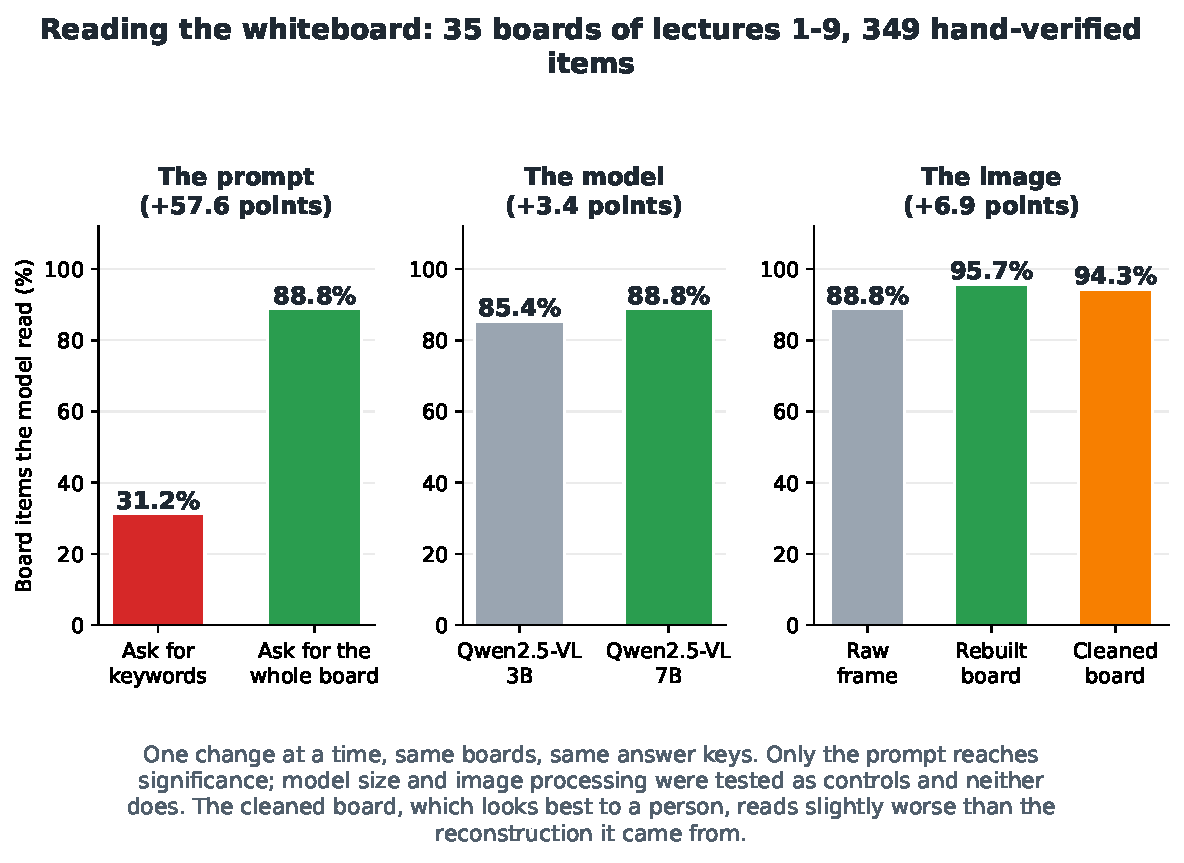
\includegraphics[width=0.9\textwidth]{fig-board-reading}
\caption{Board-content recall by item kind, keyword prompt against full
transcription, over 35 boards and 349 items. The numbers written on the board go
from none found to almost all found.}
\label{fig:fig-board-reading}
\end{figure}

Broken down by kind of item over the 35 boards, the change is from 0 of 67 numbers
to 65 of 67, from 43 of 47 names to 45 of 47, from 14 of 111 pieces of code to 90 of
111, from 47 of 94 terms to 89 of 94, and from 5 of 30 phrases to 21 of 30. The
keyword prompt found not one number on any board. This is the clearest single result
in the vision half of the thesis, and it is a result about prompting rather than
about model capability.

\textbf{The prompt was chosen on the same boards this is reported on, and that has
to be said.} There was no held-out set when the choice between the two prompts was
made. To give a figure that selection cannot explain, the boards were split by
lecture using a rule fixed before any per-half number was looked at, with the odd
numbered lectures as the development half and the even numbered ones as the test
half. The split is by lecture rather than by board because boards within a lecture
share a lecturer, a topic, a camera and a whiteboard.

\begin{table}[H]
\centering
\caption{The prompt comparison re-checked on a held-out half of the boards.}
\label{tab:promptsplit}
\small
\begin{tabular}{p{3.6cm}p{1.6cm}p{1.4cm}p{1.8cm}p{2.4cm}p{2.2cm}}
\toprule
\textbf{Half} & \textbf{Boards} & \textbf{Items} & \textbf{Keyword} &
\textbf{Full transcription} & \textbf{Better / worse} \\
\midrule
development & 17 & 173 & 34.1\% & 93.1\% & 17 / 0 \\
\textbf{test} & \textbf{18} & \textbf{176} & \textbf{28.4\%} & \textbf{84.7\%} &
\textbf{17 / 0} \\
all, the headline & 35 & 349 & 31.2\% & 88.8\% & 34 / 0 \\
\bottomrule
\end{tabular}
\end{table}

On the test half, which played no part in the choice, the full transcription prompt
still gives 28.4 per cent to 84.7 per cent, better on 17 of 18 boards and worse on
none. The honest limit of this check is that it is a split applied after the original
comparison, not a protocol registered before it, so it does not undo the original
selection. It answers the narrower question of whether the conclusion survives on
boards that played no part in choosing the prompt, and it does.

\subsection{The generated notes}
\label{sec:notes-result}

The notes were built for all 13 lectures that have hand-verified board answer keys,
in both languages, always from a transcript produced by an adapter that never heard
that lecture's lecturer. Table \ref{tab:notes} gives the recall of board content.

\begin{table}[H]
\centering
\caption{Board-content recall of the generated notes, 35 boards of the first nine
lectures, 349 items.}
\label{tab:notes}
\small
\begin{tabular}{p{6.0cm}p{2.0cm}p{5.4cm}}
\toprule
\textbf{Notes} & \textbf{Recall} & \textbf{Against the original pipeline} \\
\midrule
Original pipeline & 37.2\% & -- \\
\textbf{Annotated notes, Banglish} & \textbf{89.1\%} &
better on 32 boards, worse on 0, sign p = 4.7e-10 \\
Annotated notes, English written directly & 55.9\% &
better on 29, worse on 4, sign p = 1.1e-05 \\
Annotated notes, English translated from the Banglish & 89.4\% & -- \\
Pasting the raw board transcription into the notes & 88.0\% &
better on 30, worse on 1 \\
\bottomrule
\end{tabular}
\end{table}

\begin{figure}[H]
\centering
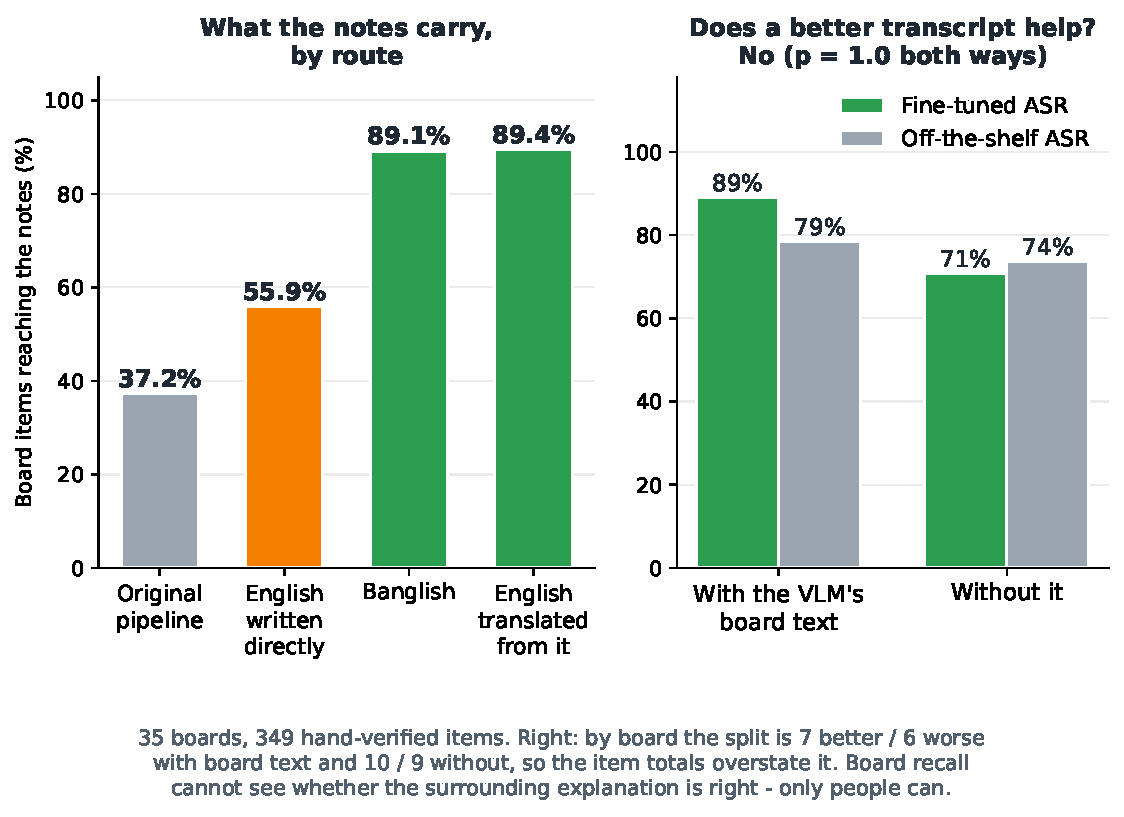
\includegraphics[width=0.9\textwidth]{fig-notes-recall}
\caption{How much of the board reaches the notes, for the original pipeline and for
the annotated notes in each language and route.}
\label{fig:fig-notes-recall}
\end{figure}

Over all 13 lectures and 436 items the Banglish notes reach 87.2 per cent and the
translated English notes 87.4 per cent. On the third lecturer's ten boards, for which
no earlier notes exist, the Banglish notes reach 79.3 per cent.

The comparison that matters most is with the row at the bottom of the table. Pasting
the vision-language model's raw board transcription into the notes reaches 88.0 per
cent, and the annotated notes reach 89.1 per cent, which a paired test cannot
separate, at 14 boards better, 8 worse and p = 0.29. That is the point rather than a
disappointment. The paste reaches its number by being a paste. The annotated notes
reach the same number while being a readable document with numbered boxes,
quotations and a step by step explanation.

\textbf{The quotation checks.} Across the 13 Banglish files the checker kept 31
quotations that appear word for word in the transcript and deleted 8 that do not, a
rejection rate of 21 per cent. The English files contain 27 quotations given as
translations, and the word-for-word check does not run on them, because a
translation cannot be matched against a Banglish transcript. The supportable claim is
therefore specific. Quotations in the Banglish notes are verified word for word
against the transcript, and quotations in the English notes are model translations
and are not verified. The claim ``every quote in the notes is verified'' would be
false and is not made anywhere in this thesis. One reference to a box that does not
exist survived across the 13 Banglish files and is counted in the output rather than
hidden.

\section{Analysis of Design Solutions}

This section analyses the design choices against the alternatives, and reports the
measurements that decided them. Four of the measurements below are negative results.

\subsection{Three approaches that did not work}

\textbf{Dual recogniser fusion.} An English recogniser and a Bengali recogniser were
run on the same nine lectures and their outputs merged. The merged output scores 73.9
per cent on the term measure against the baseline's 73.2 per cent, a difference of
0.7 percentage points, with an exact paired permutation test at p = 0.32 and a
Wilcoxon signed-rank test at p = 0.36. Four of the nine lectures get worse. The word
error rate of the merged output is 146.8 per cent against the baseline's 82.6 per
cent. The conclusion is that fusion does not fix Banglish recognition, which is what
motivated fine-tuning instead.

\textbf{Biasing the decoder towards board words.} A sweep of the bias strength from
0 to 2.0 on one lecture found term recall of 8.8 per cent with the bias off and 4.1
per cent at every non-zero setting, with the transcript truncated from 279 to 149
characters. Every non-zero strength produced byte-identical output. The shape of that
result is the finding. This is not a tuning problem with a better setting waiting to
be found, because the mechanism fails as soon as it engages. The recorded output of
the sweep gives the optimal bias as zero, so the experiment concluded against itself.

\textbf{Occlusion as a pointer.} Where the lecturer stands might indicate what the
lecture is currently about, which would give a free alignment between speech and
board regions. The test needs no manual labels. If standing in front of a region
means working on it, that region should gain more ink after the lecturer leaves than
the regions he was not standing in front of. Over 191 occlusion episodes in nine
lectures, the occluded region gained more ink in 101 cases and an unoccluded region
gained more in 81, with a Wilcoxon test at p = 0.054 and an exact sign test at p =
0.159. This does not support the claim and is reported as unsupported. The most
likely reason is that the test measures writing while a lecturer standing in front of
a region is often explaining it and adding no ink at all, which is exactly the case
where the signal would have been most useful.

\subsection{The display clean-up: a measured negative}
\label{sec:board-cleanup}

The clean-up described in Section 4.4.3 makes every board a clean white image and
was judged by eye to be better. Read by the same vision-language model with the same
prompt against the same answer keys, it is slightly worse. Table \ref{tab:cleanup}
gives the comparison.

\begin{table}[H]
\centering
\caption{The vision-language model reading the mosaic board against the cleaned
board.}
\label{tab:cleanup}
\small
\begin{tabular}{p{3.6cm}p{1.6cm}p{2.6cm}p{2.8cm}p{2.0cm}p{1.6cm}}
\toprule
\textbf{Set} & \textbf{Boards} & \textbf{Mosaic} & \textbf{Cleaned board} &
\textbf{Better / worse} & \textbf{Sign} \\
\midrule
Lectures 1 to 9 & 35 & 334/349 (95.7\%) & 329/349 (94.3\%) & 0 / 5 & p = 0.0625 \\
Third lecturer & 10 & 74/87 (85.1\%) & 71/87 (81.6\%) & 1 / 2 & p = 1.0 \\
\textbf{Combined} & \textbf{45} & \textbf{408/436 (93.6\%)} &
\textbf{400/436 (91.7\%)} & \textbf{1 / 7} & \textbf{p = 0.0703} \\
\bottomrule
\end{tabular}
\end{table}

The difference is not significant either way, so the honest statement is that there
is no measured difference, with the point estimate against the clean-up. It is not
that the clean-up is worse.

Reading the changes item by item explains the shape. The one gain is on the board the
clean-up was built for, where an end-of-era diagram that the old mask lost becomes
readable, and that board rises from 57.1 to 71.4 per cent. The losses are all single
fine details of the kind a clean-up erases, which are long code strings, a written out
sentence and two decimal numbers. There is also very little room to win, since the
mosaic is already at 95.7 per cent on the first nine lectures and 37 of the 45 boards
score identically on both.

The conclusion drawn is therefore narrow and is followed in the rest of the thesis.
The cleaned boards are kept because of how they look in a note, where every board is a
clean white image, and not because they help the model read. No claim is made that the
rebuild improved board reading, and the headline board numbers are reported on the
mosaic boards.

\subsection{Does the result need a large vision-language model?}
\label{sec:vlm-size}

The board reading was run again with Qwen2.5-VL-3B, changing nothing but the model.

\begin{table}[H]
\centering
\caption{Board reading with a 3B model against a 7B model, same prompt, same
images, same keys.}
\label{tab:vlmsize}
\small
\begin{tabular}{p{4.6cm}p{2.4cm}p{2.4cm}p{2.4cm}p{2.0cm}}
\toprule
\textbf{Boards} & \textbf{Qwen2.5-VL-3B} & \textbf{Qwen2.5-VL-7B} &
\textbf{7B better / worse} & \textbf{Sign} \\
\midrule
35 boards, 349 items & 85.4\% & 88.8\% & 11 / 5 & p = 0.21 \\
Third lecturer, 10 boards, 87 items & 77.0\% & 89.7\% & 5 / 1 & p = 0.22 \\
\textbf{Combined, 45 boards, 436 items} & \textbf{83.7\%} & \textbf{89.0\%} &
\textbf{16 / 6} & \textbf{p = 0.053} \\
\bottomrule
\end{tabular}
\end{table}

Changing the prompt is worth 57.6 percentage points, from 31.2 to 88.8. Changing the
model from 3B to 7B is worth 5.3 points, and that difference is not significant by the
sign test on either set on its own. A 3B model at 85.4 per cent already carries most of
the board. The 7B is the better model and remains the one reported, and the thesis does
not present model scale as the thing that made board reading work. This agrees with the
published finding that large multimodal models are strongly sensitive to how the
instruction is written \cite{ismithdeen2025promptception}.

The 32 billion and 72 billion parameter versions were not run, and the reason is
recorded rather than left as an omission. Their weights are 68.3 GB and 146.8 GB, the
machine had 62 GB of free disk at the time, and both would have had to be quantised to
fit in 32 GB of video memory, which would confound model size with quantisation loss.
This is therefore a comparison of a 3B model against a 7B model, and the thesis calls
it that rather than a scale study.

\subsection{Does the reconstruction help the model read the board?}

The reconstruction is a visual deliverable, and it is tempting to claim that it also
improves reading. The measurement does not support that. On the 35 boards of the first
nine lectures, recall rises from 88.8 per cent on a raw frame to 95.7 per cent on the
reconstructed board, better on 8 boards and worse on 3, with a sign test at p = 0.23
and a Wilcoxon test at p = 0.056. On the third lecturer's boards it goes the other way,
from 89.7 per cent to 85.1 per cent. This is a trend on one set and absent on the
other. The sentence this thesis uses is that the prompt is what makes the model read
the board, and the reconstruction is what makes the board usable in a note.

Two limits of the reconstruction were exposed by the hand check of the answer keys and
each deserves a sentence. Glare from the ceiling lights sits in every frame, so no
choice of frame removes it. Content that is visible in only one frame can be lost,
which happened to a binary number that was fully written at one moment, covered ten
seconds later and wiped ten seconds after that.

\subsection{Does fine-tuning the speech model improve the notes?}
\label{sec:2x2}

This is the question that joins the two halves of the thesis, and the answer is no, in
a way that needs explaining rather than hiding.

Four sets of notes were built for the 13 scored lectures, Banglish only, with
everything held constant except two things, which are whether the transcript came from
the fine-tuned model or the off-the-shelf model, and whether the board text was
supplied at all.

\begin{table}[H]
\centering
\caption{Board-content recall for the two-by-two, 35 boards, 349 items.}
\label{tab:2x2items}
\small
\begin{tabular}{p{4.6cm}p{4.0cm}p{4.0cm}}
\toprule
& \textbf{With board text} & \textbf{Without board text} \\
\midrule
\textbf{Fine-tuned transcript} & \textbf{89.1\% (311 items)} & 70.8\% (247) \\
Off-the-shelf transcript & 78.5\% (274) & 73.6\% (257) \\
\bottomrule
\end{tabular}
\end{table}

\begin{table}[H]
\centering
\caption{The same four cells counted by board, which is the test that matters.}
\label{tab:2x2boards}
\small
\begin{tabular}{p{5.6cm}p{2.2cm}p{2.6cm}p{1.6cm}p{1.6cm}}
\toprule
\textbf{Comparison} & \textbf{Item change} & \textbf{Better / worse} &
\textbf{Sign} & \textbf{Wilcoxon} \\
\midrule
With board text, base to fine-tuned & +10.6 pp & 7 / 6 & p = 1.0 & p = 0.81 \\
Without board text, base to fine-tuned & -2.8 pp & 10 / 9 & p = 1.0 & p = 0.72 \\
Fine-tuned, no board text to board text & +18.3 pp & 13 / 7 & p = 0.26 & p = 0.16 \\
Off-the-shelf, no board text to board text & +4.9 pp & 10 / 4 & p = 0.18 & p = 0.052 \\
\bottomrule
\end{tabular}
\end{table}

None of the four comparisons is significant. Read by board, the two speech conditions
split 7 to 6 with board text and 10 to 9 without it, which is as close to a coin toss
as this data can produce.

The eye-catching plus 10.6 points in the item totals is worth taking apart, because
quoting it as the benefit of fine-tuning would be wrong. Of the 37 items gained, two
boards of one lecture give 50 between them, and across the other 31 boards the
fine-tuned transcript is 13 items worse. One apparently large effect is two boards out
of thirty-five with the rest pointing gently the other way.

\textbf{Why the better transcript loses, and why that is a finding.} The two
transcripts were scored directly against the same answer keys, before any notes were
written.

\begin{table}[H]
\centering
\caption{How much of the board content each transcript already contains, 35 boards,
349 items.}
\label{tab:metricbias}
\small
\begin{tabular}{p{7.0cm}p{6.4cm}}
\toprule
\textbf{Transcript} & \textbf{Board items it contains} \\
\midrule
Off-the-shelf Whisper, character error rate 67.7\% & \textbf{106 (30.4\%)} \\
Fine-tuned Whisper, character error rate 15.8\% & 91 (26.1\%), better on 1 board,
worse on 9, sign p = 0.021 \\
\bottomrule
\end{tabular}
\end{table}

The far worse transcript contains significantly more of the board's content, and the
mechanism is mechanical rather than mysterious. Off-the-shelf Whisper translates into
English, and the answer keys are largely English technical strings such as NAND gate,
MySQL and lines of SQL. Its output is unusable as a transcript while still emitting
those exact strings. The fine-tuned model writes what the lecturer actually said, in
Banglish, and \textit{amra NAND gate dekhbo} does not string-match an English key
item. This is the same trap as the term measure discussed in Section 5.4.3. A measure
built out of English strings rewards a model that translates and penalises one that
transcribes.

\textbf{What the null result does and does not say.} It says that the fine-tuned
transcript changes almost nothing that board-content recall can see, and that measure
asks only whether facts written on the board reach the notes. It does not say the
transcript is irrelevant to note quality. The measure is blind by construction to
whether the explanation around those facts is correct, readable or even in the right
language, and the two transcripts differ enormously as transcripts. An English page
built from a transcript with 67 per cent character error will contain sentences that
are simply wrong, and nothing here measures that. Testing it properly needs readers,
which is why the reader study is the first item of future work. Until that exists, the
defensible claim is the narrow one, which is that the factual content of the notes
comes from the vision side and the speech improvement shows up in the quotations and
in the readability rather than in board recall.

\subsection{Two routes to the English notes}

Writing the English note directly from the board and the transcript gives 55.9 per
cent recall. Writing the section in Banglish first and translating it gives 89.4 per
cent, almost exactly the Banglish original's 89.1 per cent. That supports the reading
above, which is that the deficit of the direct route is the model paraphrasing the
board's strings into English prose rather than the note carrying less of the lecture.

The caveat is large and is stated with the number every time. Of the 130 items gained,
113, or 87 per cent, come from four dense boards carrying 39 to 42 items each, and
across the other 31 boards the two routes are level. Counted by board the comparison is
10 better, 7 worse and 18 tied, with a sign test at p = 0.63. There are real
regressions, with two boards falling from 6 of 7 items to 2 of 7. The statement used in
this thesis is therefore that the translated route is much better on dense,
number-heavy boards and indistinguishable from the direct route on ordinary ones.

\section{Final Design Adjustments}
\label{sec:adjustments}

Evaluation changed the design in nine places. This section lists what was changed and
what evidence forced it, and then states what is still wrong.

\subsection{Adjustments made because of a measurement}

\textbf{The loop safeguard was adopted, and then shown to be unnecessary.} Under plain
greedy decoding the small model fell into repetition loops on 58 of 184 clips, and the
loops decided the result. Whisper's compression-ratio safeguard was adopted, applied
identically to both models, and reported beside the plain numbers. With the large
model the fine-tuned system loops on one clip in 177, so the safeguard changes nothing
and the reported figures are the plain ones. Both facts are reported, including that
the safeguard was adopted after the greedy result had been seen.

\textbf{The person mask was replaced.} The original mask took whatever differed from
the usual appearance of the board, which failed when the lecturer stood still and
failed again when the camera's automatic exposure darkened a frame. It was replaced by
a pretrained segmentation network plus a shadow mask, which recovers writing the old
mask lost.

\textbf{Frames are extracted more densely for a lecturer who does not move.} Measured
in Section \ref{sec:board-coverage}.

\textbf{Each language version is written wholly in its own language.} The first design
followed a mock-up in which an English note quoted the lecturer in Banglish with a
translation beside it. Reading the first real notes showed that an English-medium
reader cannot use a Banglish quotation, so the rule was changed. This has a
consequence for what can be claimed, and the consequence is stated rather than glossed
over. The word-for-word check runs on the Banglish notes and cannot run on the English
ones.

\textbf{The English note is produced by translating the Banglish note.} Selected on the
measurement in Section 5.2.6, with the caveat about the four dense boards.

\textbf{A loop guard in the board reader.} On one board the model emitted the same
backslash line 512 times, giving 42,037 characters. Repeated identical lines are now
collapsed and the number dropped is recorded. This changes no score, because repeated
backslashes match no answer key item. It matters because that text is pasted into the
note prompt.

\textbf{A salvage parser in the board reader.} Boards carrying code make the model emit
unescaped quotation marks that break the JSON it returns, and without a fallback such a
board loses every one of its boxes. The parser now reads the fields one at a time when
the JSON cannot be parsed.

\textbf{A placeholder strip in the note builder.} Three times across 26 files the model
copied the prompt's own example text into the notes, producing a sentence of the form
\textit{The lecturer mentioned, ``exact words from the transcript''}. The quote checker
could not catch it, because it looks for quotations absent from the transcript and this
is not a quotation at all. The strip removes the prompt's placeholder text and records
how many it removed. The affected lectures were rebuilt and recall was unchanged, so
this is a readability fix rather than a scoring one.

\textbf{Label repair in the translated notes.} The translation left 97 section labels in
Banglish across the thirteen English files and returned three summary lines in capital
letters. Both are repaired by a mapping that does not call the model. The capitalisation
repair takes each word's casing from how the same file writes that word elsewhere, so
that Python, TTL and DBMS are not lower-cased.

\textbf{Normalising the Background label.} The model wrote the heading of the
non-lecture box in four different ways, and 11 of 21 boxes in one rebuild used a bare
heading with no disclaimer. Since the heading is what the reader sees, those boxes were
fenced but not labelled, which defeats the purpose of the box. The page builder now
normalises the label at render time, and all 62 boxes across the 26 pages now carry the
disclaimer.

\subsection{What is still wrong}
\label{sec:known-defects}

Four defects are known, counted and not fixed, and they are listed here rather than
left for a reader to find.

\textbf{The box finder treats a sticker as content.} The whiteboard in one room carries
a manufacturer's sticker, and because it is dark and separate the box finder puts a box
around it on every board of that lecture. It is visible in Figure
\ref{fig:board-demo-5}. It is cosmetic, it costs nothing in any measurement, and it
would be fixed by ignoring a region that appears unchanged across every era of a
lecture.

\textbf{Some quotations cannot be translated and are dropped.} On the thirteen scored
lectures the translation route kept 15 quotations and dropped 19 because it could not
produce a faithful version, and over all 42 lectures that have notes it kept 60 and
dropped 49. A dropped quotation costs the page a lecturer's voice. It is counted in the
output file of every page rather than being silent, and it is the largest remaining
defect in the English version.

\textbf{A few references to boxes that do not exist survive.} Across the 13 scored
Banglish files the box reference check removed all but one. Over all 42 lectures ten
survive in each language. They are counted, not silent.

\textbf{Four era boundaries fall in the middle of an erase.} Described in Section
\ref{sec:board-human}. The fix is to hold the era open until the wipe finishes.

\subsection{A factual error in the generated prose, found by reading}

One further defect is not a software fault and cannot be fixed by a checker. In the
notes for one digital logic lecture the model wrote that there are two types of
universal gates, which are XOR gates. The lecturer and the board both say NAND and
NOR. Board-content recall cannot catch this, because it measures whether board items
appear in the notes and not whether the prose around them is true.

This is stated here deliberately. Nothing in this thesis measures the factual
correctness of the generated explanation, the planned reader study is what would, and
an example of the error is more useful to a reader than a claim that it does not
happen.

\section{Statistical Analysis}

\subsection{Which tests were used and why}

Every comparison in this thesis is paired, because both systems are run on exactly the
same clips or the same boards. Two tests are used on every comparison. The Wilcoxon
signed-rank test ranks the differences by size and asks whether positive and negative
differences are balanced \cite{wilcoxon1945}. The exact sign test only counts how many
items improved and how many got worse, which makes fewer assumptions and is the more
conservative of the two.

Both are reported wherever they disagree, and they do disagree in places. The
two-by-two of Section \ref{sec:2x2} has one comparison at Wilcoxon p = 0.052 and sign
p = 0.18, and neither is treated as significant.

\subsection{Medians, not means, and the direction of the difference}

Two rules were adopted after being caught out by their absence.

\textbf{Report medians.} Both the base and the fine-tuned model sometimes fall into a
repetition loop and emit far more words than were spoken, which pushes a mean error
rate above 100 per cent. On one early comparison the same data gave p = 0.76 on means
and p = 2.19e-05 on medians with a paired test. The mean result was an artefact of a
handful of runaway clips, not evidence of no effect.

\textbf{Read the direction, not only the p-value.} A two-sided p-value does not say
which system won. Under plain greedy decoding one early adapter was significantly worse
than its baseline, at z = -2.62 and p = 8.7e-03, and reporting only the p-value would
have made that look like a success. The sign of the test statistic is stated beside
every p-value in this thesis.

\subsection{A metric that moves the wrong way}

The measure inherited from the earlier phase of this project is a term-based F1 over a
fixed list of 82 English words. Two independent training runs on identical data, with
the same recipe and the same seed, differing only in the order the manifest listed the
clips, gave the results in Table \ref{tab:termf1}.

\begin{table}[H]
\centering
\caption{Two training runs on identical data, showing which measures replicate.}
\label{tab:termf1}
\small
\begin{tabular}{p{4.6cm}p{3.0cm}p{3.0cm}p{2.4cm}}
\toprule
\textbf{Measure} & \textbf{Run A} & \textbf{Run B} & \textbf{Spread} \\
\midrule
Word error rate, median & 81.8\% & 77.1\% & 4.7 pp \\
Character error rate, median & 60.7\% & 57.4\% & 3.3 pp \\
Term recall & 88.8\% & 88.3\% & 0.5 pp \\
Term precision & 66.7\% & 55.3\% & \textbf{11.4 pp} \\
Term F1 & 76.1\% & 68.0\% & \textbf{8.1 pp} \\
\bottomrule
\end{tabular}
\end{table}

The speech result replicates, with both runs beating the base model at p below 0.01 on
word and character error rate. Term F1 does not, swinging 8.1 points on identical data,
driven by an 11.4 point swing in term precision.

The reason is the interesting part. Term precision counts how many of the 82 fixed
English words the model emits. Run B transcribes better Banglish, so it emits fewer
English words, so its term precision falls. The measure penalises the model for doing
the task correctly. Three consequences follow and are applied throughout this thesis. A
term F1 difference smaller than about 8 points is never claimed, which independently
rules out the fusion result of 0.7 points. Word and character error rate with their rank
tests are the headline. Both runs are reported rather than the better one being quietly
chosen.

The same effect reappears in a different place, in the note evaluation of Section
\ref{sec:2x2}, where the worse transcript contains more of the English answer key
items. Two independent instances of the same failure in one project is the reason this
thesis treats it as a finding rather than as a nuisance, and it agrees with the
published work on evaluation metrics for code-switched recognition discussed in Section
2.2.4.

\subsection{Counting by board and counting by item}

Recall over answer key items is dominated by dense boards, because a board with 42
items contributes fourteen times as much as a board with 3. Two results in this thesis
look very different depending on which is counted. The translated English route gains
130 items over the direct route, of which 113 come from four boards, and counted by
board it is 10 better and 7 worse with p = 0.63. The two-by-two gains 37 items from
fine-tuning, of which 50 come from two boards while the other 31 boards lose 13, and
counted by board it is 7 better and 6 worse with p = 1.0.

Both countings are reported for every comparison where they differ, and the by-board
count is the one the conclusion rests on.

\subsection{Multiple comparisons}

This chapter reports a large number of tests. No correction for multiple comparisons
has been applied, and that is a limitation rather than an oversight. It matters least
for the speech result, where the p-values are below 1e-30 and would survive any
correction, and it matters most for the marginal results, which is why every marginal
result in this chapter is described as a trend or as not significant rather than being
counted as a finding.

\section{Comparisons and Relationships}

\subsection{Comparison with existing systems}

Table \ref{tab:neighbours} in Chapter 2 places this work beside the four nearest
Bengali-English code-switched speech systems. The comparison cannot be made on the
numbers, and it is worth saying why clearly. Two of the four are trained and evaluated
on synthetic speech, one targets the Bengali script and one is an undocumented public
model evaluated on a random split of its own clips. Error rates on different datasets
with different transcription targets are not comparable, and this thesis does not
present them as if they were.

What can be compared is the design of the evaluation, and there this work is stricter
than its neighbours in three ways. Whole lectures are held out, so no part of a test
recording appears in training. The references are checked word by word by a person
rather than being generated. The same test is reported under two designs, one with the
test lecturers heard in training and one with an entirely unseen lecturer, so that the
easier and harder questions are separated.

For the board side, the comparison with earlier work is different in kind. Systems such
as those of Davila and Zanibbi \cite{davila2017whiteboard} and Kota et al.
\cite{kota2019generalized} extract and binarise handwriting from fixed-camera lecture
video and report component-level recall above 94 per cent on public datasets. This work
does not beat them at that task and does not attempt to. Its reconstruction is
engineering assembled from known parts. What is added is the step after it, which is
reading the reconstructed board into text with a vision-language model, scoring that
against hand-verified answer keys, and carrying numbered regions of the board into a
generated note.

\subsection{The relationship between training data and gain}

Two observations connect the amount of data to the result, and neither is a controlled
experiment.

Within the final result, the lecturer with the least training speech has by far the
worst test lecture, at 52 per cent character error against 12 to 16 per cent for the
others. Across designs, holding out an entire lecturer and training on 80 to 114
minutes gives 50.3 per cent character error, while holding out whole lectures from
known lecturers and training on 4.10 hours gives 15.8 per cent. The two differ in both
the amount of data and the difficulty of the question, so neither comparison isolates
the effect of data volume.

An earlier scaling curve on the smaller model, at 0.30, 0.60 and 0.93 hours, gave 84.6,
80.6 and 83.3 per cent word error, which is flat within the 4.5 point run-to-run noise
after the first 18 minutes and significant at every budget. A curve on the current
corpus was planned and was cancelled when the corpus closed, so the relationship
between hours and accuracy at this scale is not measured here and is listed as future
work.

\subsection{The relationship between the stages}

The clearest relationship in the results is that the factual content of a note comes
from the vision side and not from the speech side. Adding the board text moves note
recall by 18.3 points with the fine-tuned transcript and 4.9 points with the
off-the-shelf one, while changing the transcript with board text present moves nothing
that a by-board test can detect. That is not a defect of the speech work. It is a
statement about what board-content recall measures, and it is the reason the speech
result is reported on its own terms as a transcription result rather than being
justified through the notes.

\subsection{Comparison with the earlier phase of this project}

The earlier phase of the project reported a fusion improvement of 5.7 percentage
points with p = 0.003 and a large effect size, an ablation table, a bias sweep and a
set of per-video statistics. None of those numbers was produced by any code in the
project. They were re-derived where a derivation was possible and retired where it was
not. The measured fusion effect is 0.7 points at p = 0.32. The bias sweep is the one in
Section 5.2.1. Two of the ablation rows described modes the pipeline does not have. A
failure-mode breakdown of five neat percentages summing to 100 had no analysis behind
it and was removed rather than reconstructed.

This is recorded here for two reasons. It is the reason for the project rule that a
number needs a command, and a reader comparing this report with the earlier one is
entitled to know which numbers changed and why.

\section{Discussions}

\subsection{What the results mean}

The speech result is the strongest part of the thesis. Fine-tuning a large multilingual
model with a small adapter on 4.10 hours of hand-checked code-mixed classroom speech
cuts the character error rate from 67.7 to about 16 per cent on lectures the model has
never heard, with two seeds agreeing and almost every clip improving. The practical
meaning is that the output changes from something a transcriber cannot use to a draft
a transcriber can correct.

The board result is a result about prompting. The same model on the same images goes
from 31.2 to 88.8 per cent recall of what is written, purely on how it is asked, and a
model less than half the size reaches 85.4 per cent. Anyone building a system like this
should spend their effort on the prompt before spending it on a bigger model.

The note result is that board content can be made to reach the page. The annotated
notes carry 89.1 per cent of the board's items against 37.2 per cent for a
conventional summarisation prompt, and they do it while remaining a readable document
rather than a paste of extracted text.

The negative results matter as much. Fusion, decoder bias and occlusion-as-pointer were
all built and all measured, and none of them worked. The display clean-up looks better
and reads slightly worse. Fine-tuning the speech model does not move note recall.
Reporting these is what makes the positive results credible.

\subsection{Implications}

For code-mixed speech, the implication is that the data is the bottleneck and the
method is not exotic. A standard adapter on a standard model gives a large gain, and
what took the effort was five hours of carefully checked transcription and a split
design that does not leak.

For evaluation, the implication is stronger and is the part of this thesis most likely
to be useful to others. Measures assembled out of English strings systematically reward
a system that translates code-mixed speech and punish one that transcribes it. It
happened twice here in two unrelated measures, and it is consistent with the published
work on code-switched evaluation reviewed in Section 2.2.4. Anyone evaluating a
code-mixed system on an English-derived metric should check for it before believing the
result.

For classroom systems, the implication is that the whiteboard is worth the trouble.
Most of the facts a student needs from these lectures are on the board and not in the
speech, and a pipeline that reads the board recovers them.

\subsection{Limitations}

The limitations are listed together so that none has to be found by a reader.

\begin{enumerate}
  \item \textbf{No human evaluation of the notes.} The measure counts whether board
        content reached the page. It cannot see whether the explanation is correct,
        readable or useful, and a factual error in the prose has already been found by
        reading.
  \item \textbf{Three lecturers, one university, one language pair.} Nothing here shows
        that the result transfers to another institution, another subject area or
        another code-mixed pair.
  \item \textbf{5.15 hours of transcribed speech.} Small by the standards of speech
        recognition. The relationship between hours and accuracy at this scale is not
        measured.
  \item \textbf{Training is unstable at the selected learning rate.} One seed of the
        pre-registered configuration diverged completely. The stable configuration
        reported beside it was chosen after that was seen.
  \item \textbf{The board-reading prompt was chosen on the boards it is reported on.}
        A held-out half was checked afterwards and supports the conclusion, but it does
        not undo the selection.
  \item \textbf{Box finding is not evaluated.} No layout ground truth exists. It works
        well on sparse boards and coarsely on dense ones, and it draws a box around a
        sticker.
  \item \textbf{Quotations in the English notes are not verified.} They are
        translations, and the automatic check cannot apply to them.
  \item \textbf{No comparison against a neighbouring model on our own data.} Running a
        public Bengali-English model on our test clips would turn a discussion into a
        table, and it was not done before submission.
  \item \textbf{No correction for multiple comparisons.} Marginal results are described
        as trends for that reason.
  \item \textbf{The system is for recorded lectures.} Nothing here runs in real time.
\end{enumerate}

\subsection{Threats to validity}

The main threat to the speech result would be leakage between training and test. Three
things guard against it, which are whole-lecture splits, the voice check on every
recording, and the frozen record of which lectures were on each side of every split.
One leak did occur earlier in the project, it was found by the voice check, and the
affected claim was retired.

The main threat to the vision results is that the answer keys were drafted by reading
the reconstructed boards, which could favour the reconstruction over a raw frame. The
keys were then checked by a person against the board images without seeing any model
output, and the comparison between the reconstruction and the raw frame is reported as
a trend rather than a result, so the conclusion does not depend on it.

The main threat to the note results is that board-content recall is a narrow measure
that a system could game by pasting the board text into the page. That is exactly what
the variant at 88.0 per cent does, which is why the annotated notes are compared
against it rather than only against the original pipeline, and why the thesis says that
matching it while remaining readable is the claim.


\chapter{Conclusion}
% ============================================================================
% CHAPTER 6 - CONCLUSION   (template file chapter_9.tex)
% ============================================================================

\section{Summary of Findings}

This thesis set out to turn a recorded Bengali-English code-mixed whiteboard
lecture into a lecture note that a student can use. The system was built as four
stages and each stage was measured separately. The findings are summarised below in
the order they were produced.

\textbf{Off-the-shelf speech recognition does not work on this speech, and the
failure is specific.} On six held-out lectures, Whisper large-v3-turbo has a median
character error rate of 67.7 per cent and a median word error rate of 93.9 per cent.
It translates the speech into English instead of transcribing it, and it falls into
repetition loops on thirteen of the 177 test clips.

\textbf{A small adapter on the same model fixes most of that.} Trained on 4.10 hours
of hand-checked Banglish from 22 lectures, LoRA adapters bring the character error
rate down to 15.8 and 16.0 per cent in two random seeds, and the word error rate to
42.5 and 41.7 per cent. The adapted model is better on 164 and 167 of 177 clips with
p below 1e-30, and it needs no decoding safeguard, since it loops on one clip in 177.

\textbf{The gain also holds for a lecturer the model has never heard, at a lower
level.} Holding out each lecturer in turn and training on the other two cuts the
character error rate from 72.8 to 50.3 per cent, significant in all six runs. This
is the harder question and the worse number, and both designs are reported.

\textbf{Training at the selected settings is not stable.} At the learning rate the
pre-registered tuning procedure chose, one of two seeds collapsed into repetition and
produced output worse than doing nothing. The stable configuration reported beside it
is the runner-up rate from the same table, and it was run after the divergence was
seen.

\textbf{The whiteboard can be reconstructed from the video without inventing
anything.} Tiling the frame and taking each tile from a moment when the lecturer was
not in front of it gives boards in which every pixel is unmodified camera output. The
median board has 97.7 per cent of its tiles fully clear. A human check of 98 boards
found 82 complete, with writing genuinely lost on 9 and the remaining 7 explained by
the source video rather than by the method.

\textbf{Reading the board is a question of prompting, not of model size.} The same
vision-language model on the same images goes from 31.2 to 88.8 per cent recall of
hand-verified board content when the prompt asks for a full transcription instead of
keywords, and from none of 67 numbers to 65 of 67. A model less than half the size
reaches 85.4 per cent with the same prompt. The prompt is worth 57.6 points and the
model size 5.3.

\textbf{Board content can be made to reach the notes.} The annotated notes carry 89.1
per cent of the board items against 37.2 per cent for a conventional summarisation
prompt, and they match a variant that simply pastes the extracted board text, while
remaining a readable document with numbered regions, verified quotations and a
step-by-step explanation.

\textbf{Several things did not work, and that is part of the result.} Dual recogniser
fusion gives 0.7 percentage points at p = 0.32. Biasing the decoder towards board
words halves term recall at every non-zero strength. Using occlusion as a pointer to
align speech with board regions is not supported, at p = 0.054 and p = 0.159. The
display clean-up that makes boards look better makes the model read them very slightly
worse. Fine-tuning the speech model does not measurably improve board-content recall
in the notes.

\textbf{Measures built out of English strings mislead in this setting.} This appeared
twice, independently. A term-based F1 over a fixed English word list swings 8.1 points
between two training runs on identical data, and it moves against transcription
quality because a better Banglish transcript contains fewer English words. In the note
evaluation, the transcript with 67.7 per cent character error contains significantly
more of the English answer key items than the one with 15.8 per cent, for the same
mechanical reason.

\section{Contributions to the Field}

The contributions of this thesis, stated as narrowly as the evidence allows, are the
following.

\textbf{A hand-checked corpus of code-mixed classroom speech in romanized Banglish.}
Forty-four lecture recordings totalling 8.33 hours, of which 28 lectures and 5.15
hours are transcribed word by word against the audio according to a written
transcription standard, with 609 timed segments and about 39,100 words. As far as
could be found, no comparable corpus of spontaneous Bengali-English classroom speech
transcribed in the Roman alphabet existed. The nearest published corpora in this
language pair are synthetic.

\textbf{A measured speech recognition result for this variety, under a strict
evaluation design.} Whole lectures are held out, references are human, the settings
come from a procedure written down before any run, and two seeds are reported for
every configuration including the one that diverged. Two designs are reported and
labelled, one with the test lecturers heard in training and one with an entirely
unseen lecturer.

\textbf{A whiteboard reconstruction that generates nothing, read into text by a
vision-language model and scored against hand-verified answer keys.} The reconstruction
itself is engineering assembled from known parts, and the thesis says so. What is new
is the combination with a vision-language reader and the measurement of it, including
45 boards and 436 items verified by hand and 98 boards checked for missing writing.

\textbf{A demonstration that the prompt, not the model size, is what makes a
vision-language model read a handwritten board.} 57.6 points against 5.3 points, with
the choice re-checked on a held-out half of the boards.

\textbf{A note generator whose claims can be checked.} Board content is supplied as
text rather than recalled, non-lecture material is confined to a labelled box,
quotations are verified word for word against the transcript and deleted when they
fail, and references to numbered regions of the board are checked against the regions
that exist. Each of these is counted in the output file of every page.

\textbf{A methodological finding about evaluating code-mixed systems.} Measures
assembled from English strings reward a model that translates and penalise one that
transcribes. This was observed twice in unrelated measures within one project, it is
consistent with the published literature on code-switched evaluation, and it is
reported here with the mechanism and the numbers rather than as an aside.

\textbf{A set of measured negative results.} Fusion, decoder bias, occlusion-as-pointer
and the display clean-up were all built, all measured and all reported as they came
out.

\section{Recommendations for Future Work}

\subsection{The work that would most improve the thesis}

\textbf{A reader study.} This is the single most valuable missing piece. Nothing in
this thesis measures whether the notes are good to read or whether what they say is
true, and a factual error in the generated prose has already been found by reading.
The study should show about twenty students the old notes and the new notes for the
same lecture and ask which helps more, together with ratings for usefulness,
correctness and readability, giving a paired before-and-after result rather than a
score. A second arm should compare notes built from the off-the-shelf transcript with
notes built from the fine-tuned one, which is the only way to test the part of the
speech improvement that board-content recall cannot see.

\textbf{A benchmark against a neighbouring model.} Running a public Bengali-English
code-switched model on our own test clips would turn the discussion in Section 5.5.1
into a table. It costs about twenty minutes on any suitable machine and it was not
done before submission.

\textbf{Measuring post-editing effort.} The economic argument in Section 3.8.3 rests on
a projection. Timing transcribers as they correct real model drafts would replace it
with a measurement, and it is the number a department would actually want.

\subsection{Work on the speech side}

\textbf{More speech, especially from under-represented lecturers.} The lecturer with
0.7 hours in training has a test lecture at 52 per cent character error while the
others reach 12 to 16. Collecting more from that lecturer would test whether the cause
is the data or the speaker.

\textbf{A scaling curve on the current corpus.} Planned and cancelled when the corpus
closed. It would answer how much more transcription is worth buying.

\textbf{Stabilising the training.} The divergence at the selected learning rate is
reproducible enough to study. Warmup, gradient clipping or a lower alpha are the
obvious things to try, and a configuration that never diverges would be worth more than
a small gain in error rate.

\textbf{A spelling-tolerant metric as standard.} The variants computed in Section
\ref{sec:asr-spelling} were used only to answer a question. Reporting them alongside
plain error rates, and applying the same idea to the note metric, would reduce the
measurement problem described throughout this thesis.

\subsection{Work on the vision and note side}

\textbf{Hold the era open until a wipe finishes.} Four of the 98 boards were cut in the
middle of an erase. This is a small change with a known cause.

\textbf{Ignore board furniture.} A sticker that appears unchanged in every era of a
lecture should not be given a numbered box.

\textbf{Evaluate the box finding.} No layout ground truth exists, so the step that
produces the numbered regions is the one part of the pipeline with no number attached
to it.

\textbf{Notes in Bengali script.} Dropped from this thesis deliberately, because it
would be produced by translation alone and would add checking work without adding a
contribution. It is straightforward to add if a reader wants it.

\textbf{A larger notes model.} A 32 billion parameter model was intended for comparison
and was dropped for disk space. It would only change the writing, not the facts, since
it reads the extracted board text and never the board.

\subsection{Closing remark}

The system described here does what it was built to do, and the report says exactly how
well. A student can put in a recorded Banglish whiteboard lecture and get out a note
containing the lecturer's words and the lecturer's board, with the board drawn from
real pixels and the quotations checked against the transcript. The speech model is good
enough to be a draft and not good enough to be trusted unchecked. The board reading is
strong and the reason it is strong is the prompt. Whether the notes are genuinely
useful to a student is the one question this thesis cannot answer, and it is the first
thing that should be measured next.


% The contents line records whatever page is current when it runs, so it has to run
% after the page break that the bibliography starts on and before the bibliography
% itself. Placed after \printbibliography it recorded the page the bibliography ends
% on; placed before it without the \clearpage it recorded the last page of the
% preceding chapter.
\clearpage
\phantomsection
\addcontentsline{toc}{chapter}{Bibliography}
\printbibliography

% ********************************** Appendices ********************************
\newpage
\phantomsection
% These entry titles are typed by hand, so they must be kept word for word the same
% as the \chapter* headings in the appendix files themselves.
\addcontentsline{toc}{chapter}{Appendix A: The Transcription Standard}
\chapter*{Appendix A: The Transcription Standard}

Every reference transcript in this thesis was produced against the written standard
summarised here, version 1.0. The full document was given to the transcription team
before any file was written, and a validation script checks every file against it.

\section*{A.1 The segment rule}

The single most important rule is that no segment may be longer than 30 seconds,
because that is the length of audio the speech model sees at once. Anything longer is
cut by software that does not know where sentences end, which produces audio that does
not match its text. The target is 10 to 25 seconds per segment, and a break is always
taken at a natural pause, never inside a word or a phrase.

The nine transcripts produced before the standard existed do not follow this rule.
Their segments run to a median of 79 seconds and up to 225 seconds, and 98 per cent are
over 30 seconds. They are subdivided at sentence ends by the data preparation step, and
the report says so wherever they are used.

\section*{A.2 File format}

One UTF-8 text file per video, named \texttt{BanglaASR<N>\_ground\_truth.txt}, with a
header of comment lines and then one line per segment.

\begin{verbatim}
# BanglaASR12 Ground Truth Transcription
# Topic: Python Functions
# Speaker ID: B
# Video duration: 14:22
# Transcriber: RH
# Style guide version: 1.0
# ==========================================================================
[0:00-0:16] Assalamualaikum shobai. Aj amra dekhbo je kivabe python e
            function likhte hoy.
[0:16-0:33] Function mane hocche ekta code block jeta amra baar baar call
            korte pari.
\end{verbatim}

The timestamp is exactly \texttt{[M:SS-M:SS]} with no space anywhere inside the
brackets. The end timestamp of one segment is the start of the next, so there are no
gaps and no overlaps. Lines beginning with \texttt{\#} are ignored by the software.

\section*{A.3 Write it exactly as spoken}

Fillers are kept, every one of them, every time. This includes \textit{um},
\textit{uh}, \textit{aaa}, \textit{mane}, \textit{je}, \textit{tahole},
\textit{okay} and \textit{thik ache}. Three reasons were given to the team and all
three are real. The model has to learn them, and in the existing files fillers are
about 5 per cent of tokens, at 671 out of 12,890. Removing them breaks the alignment
between the text and its time window. And a reference cleaner than reality makes every
error rate reported from it wrong in our favour.

The one thing that is removed is an abandoned restart, where the lecturer begins a
sentence, stops and starts again differently. Only the finished version is kept. If it
is unclear whether something is a restart or a filler, it is kept.

The lecturer is never corrected. Slips, repeats and self-corrections are transcribed as
they happen.

\section*{A.4 Spelling}

Banglish has no spelling standard, so the guide fixes one. If one transcriber writes
\textit{kore} and another writes \textit{koree} for the same word, the model sees two
unrelated words and learns both badly. The canonical list was derived from what the
team already wrote most often, so it mostly matches their instincts. Table
\ref{tab:spellinglist} gives a sample of it.

\begin{table}[H]
\centering
\caption{A sample of the canonical spelling list. The validator enforces these.}
\label{tab:spellinglist}
\small
\begin{tabular}{p{4.0cm}p{3.0cm}p{5.0cm}}
\toprule
\textbf{Meaning} & \textbf{Use this} & \textbf{Do not write} \\
\midrule
I, my & \texttt{ami}, \texttt{amar} & amr, aami \\
we & \texttt{amra} & aamra, amraa \\
this & \texttt{eta}, \texttt{ei} & etaa, eee \\
one, a & \texttt{ekta} & ektaa, akta, ekhta \\
now & \texttt{ekhon} & ekhone, akhon \\
is happening & \texttt{hocche} & hoche, hochhe, hoicche \\
is, exists & \texttt{ache} & achhe, ase \\
if & \texttt{jodi} & zodi \\
but & \texttt{kintu} & kintuh \\
then, so & \texttt{tahole} & tahle \\
good & \texttt{bhalo} & valo, bhaalo \\
plural marker & \texttt{gula} & gulo \\
\bottomrule
\end{tabular}
\end{table}

Technical terms stay in English and are spelled in English. Text is ASCII only, with no
smart quotes and no Bengali script.

\section*{A.5 The validator}

A script checks every transcript against the rules above and reports segments over 30
seconds, unreadable timestamps, gaps and overlaps, missing headers and spellings outside
the canonical list. It can repair malformed timestamps automatically, keeping a backup
copy of the original file. The checks that would corrupt training silently, such as a
transcript with no matching video or a lecturer label that disagrees with the voice
check, are a hard gate that stops a training run before it starts.


\newpage
\phantomsection
\addcontentsline{toc}{chapter}{Appendix B: Prompts Used in the Pipeline}
\chapter*{Appendix B: Prompts Used in the Pipeline}

The results in Chapter 5 depend heavily on how the models are asked, so the three prompts
that matter are printed here as they appear in the code.

\section*{B.1 Reading the whole board}

This prompt produced the change from 31.2 to 88.8 per cent board-content recall in Section
\ref{sec:board-reading}. The prompt it replaced asked the model for keywords visible on
the board.

\begingroup\footnotesize
\begin{verbatim}
This is a photograph of a classroom whiteboard during a university lecture.

Transcribe everything written on the whiteboard, exactly as written.

- Copy every number, name, identifier, date and symbol exactly. Do not round,
  correct or reformat values.
- Write tables as Markdown tables with the same rows and columns as the board.
- Write code, SQL and program text inside ``` fences, keeping line breaks.
- Write formulas as they appear. For a bar over a term write it as NOT(...),
  for example NOT(A+B).
- Keep diagrams short: name what they are and copy any labels on them, for
  example "Gate diagram: inputs A, B into a box labelled NAND, output NOT(AB)".
- If part of the board cannot be read, write [illegible]. Never guess, and never
  add anything that is not written on the board.
- Ignore any person in the picture. Describe only what is written.

Output only the transcription.
\end{verbatim}
\endgroup

\section*{B.2 Naming and transcribing each numbered box}

The Set-of-Mark prompt of Section 4.4.3. The boxes are drawn on the image by our own code
and numbered, and the model answers per number. Boxes it names \texttt{none} are dropped,
which is how a smudge or a sticker can be removed by the model even though the box finder
created it.

\begingroup\footnotesize
\begin{verbatim}
This is a classroom whiteboard from a university lecture. Numbered coloured boxes
have been drawn on it; each box surrounds one part of the writing. There are {n}
boxes, numbered 1 to {n}.

For every box, reply with:
- "id": the box number.
- "name": 1 to 4 words saying what kind of content the box holds, for example
  "Title", "Definition", "Truth table", "Gate symbol", "Block diagram",
  "SQL query", "Code", "List", "Worked example", "Formula". If the box holds no
  lecture writing (a smudge, a shadow, a logo or sticker, the edge of the board),
  use "none".
- "text": everything written inside that box, copied exactly: every number, name
  and symbol. For a bar over a term write NOT(...). Write a table as Markdown
  table rows. Write [illegible] for what cannot be read. Never guess.

Reply with JSON only: a list with one object per box, in box order, like
[{"id": 1, "name": "Title", "text": "Digital Logic Design"}]
\end{verbatim}
\endgroup

\section*{B.3 Writing one section of the notes}

These rules are shared by both languages. Rule 1 is the direct answer to the textbook
recitation described in Section 1.3, and rule 2 is what makes the notes point at the
numbered boxes.

\begingroup\footnotesize
\begin{verbatim}
RULES
1. Teach what THIS lecturer taught, with the lecturer's own examples and values.
   Explain it properly, for a student who missed the class: walk through each step
   on the board, say what it means and why the lecturer does it in that order, and
   spell out anything the board only shows as a symbol. What is not wanted is
   material from elsewhere: every fact in the explanation must come from the board
   or the transcript. Anything else belongs in the BACKGROUND section, never mixed
   in.
2. The board has numbered coloured boxes, listed below. Point the student at them,
   for example "Look at the orange box 3" or "the truth table in box 5". Use only
   the box numbers that are listed, and mention every listed box at least once.
3. Copy numbers, names, code, formulas and table values exactly as they appear in
   the box text. A wrong value is worse than a missing one.
4. The transcript is machine-made and has errors. Where it is garbled, rely on the
   board. Never invent what the lecturer said.
5. No greetings, no filler, no "in this section".
6. A table on the board is written as a Markdown table, never described row by row.
7. Plain text for formulas and symbols: A + B, (A + B)', NOT(A + B), A XOR B.
\end{verbatim}
\endgroup

The quotation instruction differs by language. The Banglish note quotes the lecturer's
real words, so the quotation can be checked against the transcript character by character,
and a quote that is not word for word in the transcript is deleted automatically. The
English note is read by a student who cannot read Banglish, so the lecturer is quoted in
English translation; a translation cannot be matched against a Banglish transcript, so the
automatic checker does not run on those files and each file records that fact in its
footer.

The example line in the Banglish quotation instruction, \texttt{"exact words from the
transcript"}, was itself copied into the notes as if it were a real quotation three times
across 26 files. The quotation checker could not catch it, because it looks for quotations
absent from the transcript and this is not a quotation at all, so a separate step now
removes the prompt's own placeholder text and counts how many it removed.


\end{document}
